\documentclass[11pt,twoside,openright]{book}

%==============================================================
% PACKAGES
%==============================================================
\usepackage[utf8]{inputenc}
\usepackage[T1]{fontenc}
\usepackage{lmodern}
\usepackage[english]{babel}
\usepackage{geometry}
\geometry{a4paper,margin=2.7cm}

\usepackage{graphicx}
\usepackage{xcolor}
\usepackage{tikz}
\usetikzlibrary{shapes.geometric,arrows.meta,positioning,fit,backgrounds,calc,decorations.pathreplacing}

\usepackage{amsmath,amssymb,amsthm}
\usepackage{booktabs}
\usepackage{longtable}
\usepackage{array}
\usepackage{enumitem}
\usepackage{listings}
\usepackage{fancyhdr}
\usepackage{titlesec}
\usepackage{epigraph}
\usepackage{microtype}
\usepackage[hidelinks,colorlinks=true,linkcolor=black,citecolor=black,urlcolor=blue!50!black]{hyperref}
\usepackage{cleveref}
\usepackage{tcolorbox}
\tcbuselibrary{listings,skins,breakable}
\usepackage{appendix}

%==============================================================
% COLORS
%==============================================================
\definecolor{dagonblue}{RGB}{20,60,110}
\definecolor{dagongray}{RGB}{245,245,245}
\definecolor{dagonaccent}{RGB}{0,110,130}
\definecolor{codebg}{RGB}{248,248,250}
\definecolor{codeframe}{RGB}{200,200,210}

%==============================================================
% CODE LISTINGS
%==============================================================
\lstdefinestyle{python}{
  language=Python,
  backgroundcolor=\color{codebg},
  basicstyle=\ttfamily\footnotesize,
  keywordstyle=\color{dagonblue}\bfseries,
  commentstyle=\color{gray}\itshape,
  stringstyle=\color{dagonaccent},
  numbers=left,
  numberstyle=\tiny\color{gray},
  stepnumber=1,
  numbersep=8pt,
  frame=single,
  rulecolor=\color{codeframe},
  breaklines=true,
  breakatwhitespace=false,
  showstringspaces=false,
  tabsize=2,
  captionpos=b,
  xleftmargin=1em,
  framexleftmargin=0.8em
}
\lstdefinestyle{bash}{
  language=bash,
  backgroundcolor=\color{codebg},
  basicstyle=\ttfamily\footnotesize,
  keywordstyle=\color{dagonblue}\bfseries,
  commentstyle=\color{gray}\itshape,
  stringstyle=\color{dagonaccent},
  frame=single,
  rulecolor=\color{codeframe},
  breaklines=true,
  showstringspaces=false,
  xleftmargin=1em
}
\lstdefinestyle{ini}{
  backgroundcolor=\color{codebg},
  basicstyle=\ttfamily\footnotesize,
  keywordstyle=\color{dagonblue}\bfseries,
  commentstyle=\color{gray}\itshape,
  frame=single,
  rulecolor=\color{codeframe},
  breaklines=true,
  showstringspaces=false,
  xleftmargin=1em
}
\lstset{style=python}

%==============================================================
% THEOREM-LIKE / PEDAGOGICAL ENVIRONMENTS
%==============================================================
\newtcolorbox{definitionbox}[1]{
  colback=dagongray, colframe=dagonblue, fonttitle=\bfseries,
  title={Definition: #1}, breakable, boxrule=0.6pt, arc=1mm
}
\newtcolorbox{practicebox}[1][Scientific Practice Note]{
  colback=white, colframe=dagonaccent, fonttitle=\bfseries,
  title={#1}, breakable, boxrule=0.6pt, arc=1mm
}
\newtcolorbox{cautionbox}[1][Caution]{
  colback=red!4, colframe=red!55!black, fonttitle=\bfseries,
  title={#1}, breakable, boxrule=0.6pt, arc=1mm
}
\newtcolorbox{lessonbox}[1]{
  colback=blue!3, colframe=dagonblue, fonttitle=\bfseries\large,
  title={#1}, breakable, boxrule=0.8pt, arc=1mm
}

\theoremstyle{definition}
\newtheorem{example}{Example}[chapter]
\newtheorem{exercise}{Exercise}[chapter]

%==============================================================
% HEADERS
%==============================================================
\pagestyle{fancy}
\setlength{\headheight}{14.5pt}
\fancyhf{}
\fancyhead[LE,RO]{\thepage}
\fancyhead[RE]{\nouppercase{\leftmark}}
\fancyhead[LO]{\nouppercase{\rightmark}}
\renewcommand{\headrulewidth}{0.4pt}

\titleformat{\chapter}[display]
  {\normalfont\huge\bfseries\color{dagonblue}}
  {\chaptertitlename\ \thechapter}{20pt}{\Huge}
\titleformat{\part}[display]
  {\normalfont\Huge\bfseries\color{dagonblue}\centering}
  {\partname\ \thepart}{20pt}{\Huge}

%==============================================================
% TITLE DATA
%==============================================================
% Version number, date and history of the book: front/version.tex.
% Version of the book, in semantic versioning (MAJOR.MINOR.PATCH).
%
%   MAJOR  a new edition: the course is realigned with a new DAGonStar release,
%          or parts and chapters are reorganized
%   MINOR  new chapters, sections, examples or appendices
%   PATCH  corrections that change no structure
%
% Bump \bookversion and \bookdate, add a row to \bookhistory, then tag the
% commit v<version>: the release workflow refuses a tag that differs from
% \bookversion.  The date is fixed here, not \today, so that a rebuild of the
% same sources gives the same title page.
\newcommand{\bookversion}{1.0.0}
\newcommand{\bookdate}{21 November 2026}
\newcommand{\bookhistory}{%
  1.0.0 & 21 November 2026 & First versioned edition, titled \emph{Workflows in
    Practice with DAGonStar}; environmental computational science, on the Gulf of
    Naples dataset, as the use case of the whole book; aligned with
    DAGonStar~3.0.0. \\
}

\hypersetup{
  pdftitle={Workflows in Practice with DAGonStar},
  pdfsubject={Orchestrating AI-HPC Workflows for Computational Science, version \bookversion},
  pdfauthor={Raffaele Montella},
  pdfkeywords={DAGonStar, scientific workflows, AI-HPC, environmental computational science}
}
\fancyfoot[C]{\footnotesize\color{gray}Version \bookversion}

\title{
  \vspace{-2.8cm}
  {\Huge\bfseries Workflows in Practice with DAGonStar}\\[0.6em]
  {\Large Orchestrating AI--HPC Workflows for Computational Science}\\[1.2em]
  {\large A Textbook on Scientific Workflow Engineering}\\[0.4em]
  {\normalsize\itshape Use case: environmental computational science}\\[1.2em]
  % Cover image: the DAGonWeb workflow editor (Apache-2.0, credited in front/colophon.tex).
  \fcolorbox{codeframe}{white}{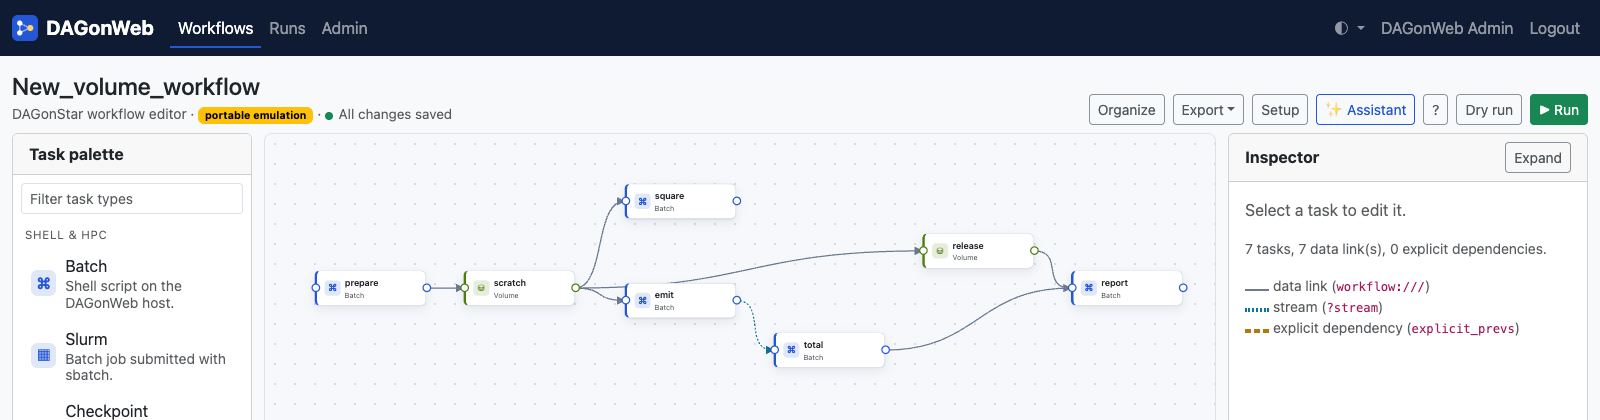
\includegraphics[width=0.88\textwidth]{figures/dagonweb-cover}}\\[0.3em]
  {\footnotesize\color{gray}Designing a DAGonStar workflow in DAGonWeb}
}
\author{
  Prof.\ Raffaele Montella \\
  \small High-Performance Scientific Computing Laboratory \\
  \small Department of Science and Technology \\
  \small University of Naples ``Parthenope'' \\
  \small \texttt{raffaele.montella@uniparthenope.it} \\[1.2em]
  % Contributors, in alphabetical order of surname.
  \normalsize\textbf{Contributors} \\[0.4em]
  \footnotesize
  \begin{tabular}{@{}r@{\quad}l@{}}
    Juan Armando Barrón Lugo & Center for Research and Advanced Studies of the National \\
      & Polytechnic Institute, Cinvestav Unidad Tamaulipas, Mexico \\[0.3em]
    Ciro Giuseppe De Vita & Department of Science and Technology, \\
      & University of Naples Parthenope, Italy \\[0.3em]
    Diana Di Luccio & Department of Science and Technology, \\
      & University of Naples Parthenope, Italy \\[0.3em]
    Dante Domizzi Sánchez-Gallegos & Department of Computer Science, \\
      & University Carlos III of Madrid, Spain \\[0.3em]
    Genaro Domizzi Sánchez-Gallegos & Department of Computer Science, \\
      & University Carlos III of Madrid, Spain \\[0.3em]
    Catherine Alessandra Torres Charles & Department of Computer Science, \\
      & University Carlos III of Madrid, Spain
  \end{tabular} \\
  \rule{0pt}{2.2em}\small \textit{Companion textbook of the 48-lecture course, aligned with DAGonStar 3.0.0}
}
\date{Version \bookversion\ --- \bookdate}

%==============================================================
% DOCUMENT
%==============================================================
\begin{document}

\frontmatter
\maketitle
% Verso of the title page: version, licence and version history.
\thispagestyle{empty}
\vspace*{\fill}
\begin{flushleft}
\small
\textbf{Workflows in Practice with DAGonStar}\\
Orchestrating AI--HPC Workflows for Computational Science\\[1em]

\textbf{Version} \bookversion\ (\bookdate)\\
Aligned with DAGonStar~3.0.0 (\url{https://github.com/DagOnStar/dagonstar}).\\[1em]

The version number follows \emph{MAJOR.MINOR.PATCH}: a new major version is a
new edition, a new minor version adds material, a new patch version corrects
it. Each version is published as a tagged release of the course repository,
with the PDF named \texttt{Workflows\_in\_Practice\_with\_DAGonStar.pdf}.\\[1em]

\textbf{Use case.} The examples of this book are drawn from environmental
computational science. The running case is the hourly observations of three
coastal stations of the Gulf of Naples (\texttt{NAP} Naples, \texttt{CAP} Capri, \texttt{ISC} Ischia)
on 2 November 2026, processed by workflows that grow from a single task to an
AI--HPC pipeline.\\[1em]

Released under CC0~1.0: no rights reserved.\\[1.5em]

\textbf{Version history}\\[0.3em]
\begin{tabular}{@{}l@{\quad}l@{\quad}p{0.62\linewidth}@{}}
\toprule
\textbf{Version} & \textbf{Date} & \textbf{Changes} \\
\midrule
\bookhistory
\bottomrule
\end{tabular}
\end{flushleft}
\clearpage


\chapter*{Abstract}
\addcontentsline{toc}{chapter}{Abstract}

This textbook presents \emph{DAGonStar} (Direct Acyclic Graph On anything, also
written \emph{DAGon*}), a lightweight Python workflow engine designed to
orchestrate computational tasks across local machines, on-premise
high-performance computing (HPC) clusters, containers, cloud-based virtual
infrastructures, and, in its current evolution, artificial-intelligence (AI)
and web services. The material is the companion textbook of a 48-lecture course in which
theory and hands-on work are mixed in every lecture. It is aligned with
DAGonStar~3.0.0 (\url{https://github.com/DagOnStar/dagonstar}).

The book follows the four parts of the course. Part~I (Lectures~01--12)
establishes the foundations of scientific workflow orchestration: directed
acyclic graphs, the \texttt{workflow://} schema, configuration, scratch
folders, cycle detection and a first station pipeline. Part~II
(Lectures~13--24) covers execution, data and recovery: staging, garbage
collection, checkpointing, failures, native tasks, asynchronous runs,
meta-workflows, sweeps and ensembles. Part~III (Lectures~25--36) presents the
task models for AI--HPC integration: Web, LLM, FaaS, IoT and agentic tasks,
joined across the computing continuum, and an environmental case study.
Part~IV (Lectures~37--48) turns to infrastructure, data movement and FAIR
practice: containers, orchestrators, remote and cloud hosts, Slurm, BeeOND,
pre-staging, data movers, FAIR metadata, CWL export, operations and a
capstone. Appendices~A--D collect the API reference, developer practices,
configuration reference and checkpoint semantics. Appendix~E presents
DAGonFS, an in-memory MPI-distributed file system for workflow scratch data.
Appendices~F--H cover three additions around DAGonStar~3.0: ad-hoc volumes
shared by volume tasks and streams, meta-tasks that run workflows written for
other engines, and DAGonWeb, the web interface for designing and running
DAGonStar workflows.

Every course example is included verbatim from the \texttt{examples/}
folder of the course repository, together with its recorded output. The
script \texttt{tools/run\_examples.py} re-runs every example against the
installed DAGonStar and compares the outputs, so the book stays consistent
with the code.

\tableofcontents
\listoffigures
\lstlistoflistings

\chapter*{Preface}
\addcontentsline{toc}{chapter}{Preface}

Computational environmental science increasingly depends on the orchestration
of heterogeneous resources: numerical models compiled for HPC clusters, data
preprocessing and post-processing scripts, container images that freeze a
fragile scientific software stack, cloud instances rented for a single
forecast cycle, and --- more recently --- AI services consumed through web
APIs for summarization, anomaly detection, or decision support. The challenge
this book addresses is not how to write any one of these components, but how
to make their \emph{composition} explicit, reproducible, portable, and
auditable.

\emph{DAGonStar} answers this challenge with a deliberately small abstraction:
a workflow is a directed acyclic graph (DAG) of tasks, and a task is a Python
object that executes a command --- local, remote, containerized,
scheduler-submitted, an HTTP request, an LLM completion, or an importable
Python function --- in a particular environment. This minimalism is the
engine's central design virtue. It keeps workflow authoring close to ordinary
Python, while still providing the scientific guarantees that ad hoc shell
scripts cannot: explicit dependency graphs, automatic data staging, cycle
detection, checkpointing, and a uniform mechanism --- the \texttt{workflow://}
schema --- for expressing that one task consumes a file produced by another.

\paragraph{How this book is organized.}
The book accompanies a course of 48 lectures plus one appendix lecture. Each
lecture has a slide deck of 30 slides (\texttt{en/lectures/}), speaker notes
(\texttt{en/notes/}) and one or more runnable examples
(\texttt{examples/NN-topic/}). Theory and hands-on work are not separated:
every lecture introduces a concept and runs it immediately. The chapters
group the lectures into four parts, and \Cref{tab:course-map} shows where
each lecture is treated.

\begin{table}[h]
\centering
\small
\begin{tabular}{@{}lp{0.47\linewidth}p{0.30\linewidth}@{}}
\toprule
\textbf{Lectures} & \textbf{Topics} & \textbf{Chapters} \\
\midrule
01--05 & Workflows, script vs DAG, architecture, environment, configuration &
  \ref{ch:introduction}--\ref{ch:getting-started}, \ref{ch:configuration} \\
06--10 & First task, DAGs, dataflow, cycles, scratch folders &
  \ref{ch:lessons-01-02}, \ref{ch:schema}, \ref{ch:lessons-03-04} \\
11--12 & Inspection, station pipeline & \ref{ch:course-pipeline} \\
13, 15 & Staging, checkpoints & \ref{ch:lessons-05-07} \\
14, 16, 19--21, 23--24 & Garbage collection, failures, bindings, sweeps,
  ensembles, dry runs & \ref{ch:resilient} \\
17, 22 & Asynchronous runs, meta-workflows & \ref{ch:meta-async} \\
18 & Native tasks & \ref{ch:native-tasks} \\
25--28 & Web and LLM tasks & \ref{ch:web-tasks}, \ref{ch:llm-tasks} \\
29--36 & FaaS, IoT, agentic tasks, continuum & \ref{ch:faas-iot-agentic} \\
37, 41 & Docker, Slurm & \ref{ch:backends} \\
38--40, 42--44 & Apptainer, orchestrators, remote and cloud, BeeOND,
  pre-staging, movers & \ref{ch:hpc-storage} \\
45--48 & FAIR, CWL, operations, capstone & \ref{ch:fair-cwl} \\
A1 & DAGonFS & Appendix~\ref{app:dagonfs} \\
A2 & Ad-hoc volumes and streams & Appendix~\ref{app:volumes} \\
A3 & Meta-tasks & Appendix~\ref{app:meta-tasks} \\
A4 & DAGonWeb & Appendix~\ref{app:dagonweb} \\
\bottomrule
\end{tabular}
\caption{Course map: lectures and the chapters that treat them.}
\label{tab:course-map}
\end{table}

Chapters on external software (\Cref{ch:external-software}), the
environmental case study (\Cref{ch:case-study}), the examples catalog
(\Cref{ch:examples-catalog}) and the synthesis (\Cref{ch:synthesis}) connect
the lectures to research practice. Appendices~A--D collect reference
material: the public API, developer practices, the configuration model and
checkpoint semantics. Appendix~E presents DAGonFS, Appendix~F ad-hoc volumes
and streams, Appendix~G meta-tasks and Appendix~H DAGonWeb.

\paragraph{Intended audience.}
This book is written for graduate students, researchers, and research software
engineers in computational and environmental science who need to compose
heterogeneous computational pipelines reproducibly. Working knowledge of
Python and of basic Unix/HPC concepts (shells, SSH, job schedulers) is
assumed; no prior exposure to workflow engines is required.

\paragraph{A note on fidelity to the software.}
Every course example is included in this book with \texttt{lstinputlisting}
from the course repository, and so is its recorded output. The examples were
written for and checked against DAGonStar~3.0.0
(\url{https://github.com/DagOnStar/dagonstar}). The script
\texttt{tools/run\_examples.py} runs them all again and reports any output
that differs from the recorded one. Where the software has a limitation,
such as name-based checkpoint reuse (\Cref{ch:resilient}), the book shows it
rather than smoothing it away.


\mainmatter

\part{Foundations (Lectures 01--12)}
\chapter{Introduction to Scientific Workflows}
\label{ch:introduction}

\epigraph{If these steps remain implicit in shell history, personal notebooks,
or site-specific scripts, the experiment is difficult to audit. Workflow
systems make the structure explicit.}{\textit{DAGonStar documentation,
Introduction to Scientific Workflows}}

\section{Why Workflows Matter in Computational Science}

Modern computational science rarely consists of a single program executed
once. A realistic environmental-science experiment, for instance, combines
many heterogeneous activities:

\begin{itemize}[leftmargin=1.4em]
  \item preprocessing observational data;
  \item running models or simulations;
  \item staging intermediate files between machines;
  \item executing tools on HPC clusters or cloud instances;
  \item post-processing model products;
  \item publishing scientific outputs;
  \item preserving sufficient context to reproduce a result.
\end{itemize}

When these steps are encoded only in shell history, ad hoc notebooks, or
site-specific scripts passed from one student to the next, the resulting
experiment is opaque: it cannot easily be audited, repeated by a different
researcher, or ported to a different machine. A \emph{workflow system} exists
precisely to make this implicit structure explicit, executable, and
inspectable.

DAGonStar approaches the problem with a deliberately small abstraction: a
\textbf{workflow is a directed acyclic graph (DAG) of tasks}, and each
\textbf{task} is a Python object that executes a command in a particular
environment. The remainder of this chapter develops this abstraction
formally and explains the scientific benefits it is designed to deliver.

\subsection{The Scientific Benefits of Explicit Workflows}

The DAGonStar documentation identifies five principal benefits that follow
from making computational structure explicit:

\begin{description}[leftmargin=1.6em,style=nextline]
  \item[Reproducibility] the sequence of computations is encoded as source
    code, not as institutional memory.
  \item[Traceability] inputs, outputs, and task dependencies are visible as
    first-class graph structure rather than buried in script side effects.
  \item[Portability] the same workflow structure can target different
    execution backends --- a laptop today, an HPC cluster tomorrow --- without
    rewriting the scientific logic.
  \item[Parallelism] independent tasks can run concurrently when resources
    permit, because the dependency graph makes independence explicit.
  \item[Recoverability] checkpointing can avoid recomputing finished work
    after a partial failure, which matters enormously for expensive
    simulations.
\end{description}

\begin{practicebox}
Even apparently small automation gains compound at scale. A workflow that
takes ten extra minutes to encode explicitly, instead of being run by hand
from a terminal, pays for itself the first time it must be rerun --- with a
different parameter, on a different machine, or six months after the original
researcher has left the project.
\end{practicebox}

\section{Directed Acyclic Graphs}
\label{sec:dag-theory}

\begin{definitionbox}{Directed Acyclic Graph (DAG)}
A \emph{directed acyclic graph} $G = (V, E)$ consists of a finite set of
\textbf{nodes} $V$ and a set of directed \textbf{edges} $E \subseteq V \times
V$, such that there is no sequence of edges
$v_1 \to v_2 \to \dots \to v_k \to v_1$ that returns to its starting node. In
scientific workflow terminology:
\begin{itemize}
  \item a \textbf{node} is a computational \emph{task};
  \item an \textbf{edge} $(u,v) \in E$ means that task $v$ \emph{depends on}
    task $u$, i.e.\ $u$ must complete before $v$ may begin;
  \item \textbf{acyclic} means the graph contains no circular dependency.
\end{itemize}
\end{definitionbox}

The acyclicity constraint is not a mathematical nicety: it is the precise
condition under which a valid execution order (a \emph{topological sort})
exists. If a cycle were permitted, no task in the cycle could be scheduled
first without violating some dependency in the cycle, and the workflow would
be unrealizable.

\begin{figure}[h]
\centering
\begin{tikzpicture}[
  node distance=16mm and 22mm,
  task/.style={rectangle, rounded corners, draw=dagonblue, very thick,
    fill=blue!4, minimum width=20mm, minimum height=9mm,
    font=\sffamily\bfseries},
  arr/.style={-{Stealth[length=2.6mm]}, thick, dagonblue}
]
  \node[task] (A) {Tokio};
  \node[task, right=of A] (D) {Mosco};
  \node[task, above=of D] (B) {Berlin};
  \node[task, below=of D] (C) {Nairobi};
  \draw[arr] (A) -- (B);
  \draw[arr] (A) -- (C);
  \draw[arr] (B) -- (D);
  \draw[arr] (C) -- (D);
\end{tikzpicture}
\caption{A four-task DAG corresponding to the engine's canonical
``Batch Task Flow'' example. \texttt{Tokio} has no predecessors and runs
first; \texttt{Berlin} and \texttt{Nairobi} depend only on \texttt{Tokio} and
may run concurrently; \texttt{Mosco} depends on both and runs last.}
\label{fig:basic-dag}
\end{figure}

\Cref{fig:basic-dag} illustrates the canonical example used throughout the
DAGonStar project, expressed as four \texttt{BATCH} tasks: \texttt{Tokio}
writes a file consumed implicitly by \texttt{Mosco}, while \texttt{Berlin} and
\texttt{Nairobi} are independent siblings that both depend only on
\texttt{Tokio}. The graph immediately exposes the available parallelism: a
scheduler is free to run \texttt{Berlin} and \texttt{Nairobi} concurrently
once \texttt{Tokio} finishes.

DAGonStar validates the workflow graph before execution, either implicitly
when dependencies are constructed through \texttt{Workflow.make\_dependencies()},
or explicitly via \texttt{Workflow.Validate\_WF()}. A cycle is treated as a
\emph{modeling error}: the engine refuses to run a workflow whose dependency
graph is not a true DAG.

\section{Task-Oriented and Data-Oriented Workflows}
\label{sec:task-vs-data}

DAGonStar supports two complementary ways of describing a workflow, and the
distinction between them is the single most important conceptual choice a
workflow author makes.

\subsection{Task-Oriented Workflows}

In a \textbf{task-oriented workflow}, dependencies are stated explicitly by
the author, independent of any file the tasks happen to exchange:

\begin{lstlisting}[caption={Explicit dependency declaration.}]
task_b.add_dependency_to(task_a)
\end{lstlisting}

This statement reads: ``\texttt{task\_b} must wait for \texttt{task\_a}.''
Explicit dependencies are appropriate when the relationship between two tasks
is \emph{conceptual or procedural} rather than a literal file consumption ---
for example, ``validate parameters before launching the model.''

\subsection{Data-Oriented Workflows}

In a \textbf{data-oriented workflow}, dependencies are \emph{inferred} from
the command text using the \texttt{workflow://} schema (developed fully in
\Cref{ch:schema}):

\begin{lstlisting}[caption={Implicit, data-driven dependency.}]
task_b = DagonTask(TaskType.BATCH, "B", "cat workflow:///A/output/result.txt")
\end{lstlisting}

When \texttt{Workflow.make\_dependencies()} is called, DAGonStar scans every
task's command string, finds the reference to task \texttt{A}, records the
dependency $A \to B$, and later stages the referenced file into \texttt{B}'s
working directory before \texttt{B} executes.

\begin{practicebox}
The data-oriented style is especially natural for scientific pipelines,
because dependency edges then follow the \emph{data products} being consumed
--- which is, after all, how a scientist already thinks about a processing
chain: ``the post-processing step needs the simulation's NetCDF output,''
not ``task three must follow task two for an unstated reason.''
\end{practicebox}

Both styles may, and routinely do, coexist in the same workflow: explicit
edges encode procedural ordering, while \texttt{workflow://} edges encode
genuine data lineage. \Cref{ch:lessons-01-02} develops both patterns with
complete, runnable examples.

\section{DAGonStar's Computational Model}
\label{sec:computational-model}

The current implementation centers on a small number of cooperating
abstractions, summarized here and developed individually across the
remainder of Part~I and Part~II:

\begin{description}[leftmargin=2.2em,style=nextline]
  \item[\texttt{Workflow}] the container and scheduler for a set of tasks;
    owns dependency construction, execution, checkpoint state, and
    configuration.
  \item[\texttt{DagonTask}] a \emph{factory} that constructs a concrete task
    implementation from a \texttt{TaskType} value.
  \item[\texttt{Task}] the base class providing threaded task execution,
    dependency bookkeeping, and \texttt{workflow://} resolution.
  \item[\texttt{Batch}] a local shell task --- the simplest concrete
    execution backend.
  \item[\texttt{Slurm}] a task submitted through \texttt{sbatch} to an HPC
    job scheduler.
  \item[\texttt{RemoteTask}] a task executed on a remote host through SSH.
  \item[\texttt{DockerTask}] a task executed inside a Docker container.
  \item[\texttt{CloudTask}] a task bound to an Apache Libcloud-managed cloud
    instance.
  \item[\texttt{Stager}] the component responsible for generating or
    invoking the data-movement operation between two dependent tasks.
\end{description}

Operationally, the workflow engine runs tasks as Python \texttt{threading.Thread}
objects. Each task thread waits for its predecessors, prepares its scratch
directory, resolves data references, executes its generated launcher script,
updates its status, and finally releases the tasks that depend on it. This
execution model is examined in full mechanical detail in
\Cref{ch:architecture}.

\section{The Role of Scratch Directories}

Scientific workflows frequently produce many intermediate files. DAGonStar
therefore gives \emph{every} task its own working directory, called a
\textbf{scratch directory}. The base path for all scratch directories is set
once, in configuration:

\begin{lstlisting}[style=ini,caption={Minimal scratch directory configuration.}]
[batch]
scratch_dir_base=/tmp/
\end{lstlisting}

If a task is not given an explicit \texttt{working\_dir}, DAGonStar
constructs one automatically from the workflow's scratch base and a
timestamped task name (for example, \texttt{/tmp/1710000000000-prepare}).
Every task additionally receives an internal \texttt{.dagon/} directory
containing its generated launcher script and execution metadata --- a
mechanism examined closely in \Cref{ch:lessons-03-04}.

\section{Execution Backends at a Glance}

DAGonStar's public task types are enumerated in \texttt{dagon.task.TaskType}.
There are sixteen in DAGonStar~3.0.0 (\texttt{examples/03-architecture}); the
main ones are:

\begin{center}
\begin{tabular}{@{}ll@{}}
\toprule
\textbf{\texttt{TaskType}} & \textbf{Execution environment} \\
\midrule
\texttt{BATCH}      & Local (or remote, via SSH keyword arguments) shell command \\
\texttt{SLURM}       & HPC job-scheduler submission via \texttt{sbatch} \\
\texttt{CLOUD}       & Apache Libcloud-managed virtual machine \\
\texttt{DOCKER}      & Containerized execution via the Docker SDK \\
\texttt{LLM}         & OpenAI-compatible Chat Completions request \\
\texttt{NATIVE}      & Importable Python \texttt{module:function} call \\
\texttt{WEB}         & Arbitrary HTTP/HTTPS request \\
\texttt{CHECKPOINT}  & Explicit checkpoint-preservation task \\
\texttt{META}        & A workflow of another engine, run unmodified (Appendix~\ref{app:meta-tasks}) \\
\texttt{VOLUME}      & Creates or destroys a shared ad-hoc volume (Appendix~\ref{app:volumes}) \\
\bottomrule
\end{tabular}
\end{center}

Remote variants of several task types are selected not by a different
\texttt{TaskType} value, but by \emph{keyword arguments}: for example, a
\texttt{BATCH} task constructed with \texttt{ip=...} becomes a remote batch
task transparently. This design keeps workflow code compact while still
exposing several execution environments through one uniform factory,
\texttt{DagonTask}. It also means that several integrations are
\emph{optional}: using Docker, cloud, Globus, or remote SSH execution
requires the corresponding site-specific service or credential, while the
core local-batch engine has no such external dependency.

\begin{practicebox}
\texttt{LLM} tasks --- the engine's principal AI integration point --- call
configured OpenAI-compatible Chat Completions providers and can consume local
UTF-8 producer files through the same \texttt{workflow://} schema used by
ordinary file-based tasks. This is the technical mechanism that allows an AI
inference step to sit inside the same DAG as a numerical simulation, with the
same dependency, staging, and provenance guarantees. \Cref{ch:llm-tasks} is
devoted entirely to this mechanism.
\end{practicebox}

\section{Workflows in the Landscape of Computational Science}

It is useful, before going further, to situate the workflow-orchestration
problem within the broader history of computational science tooling, so
that the design choices examined in later chapters can be understood not as
arbitrary engineering preferences but as responses to a recurring,
well-documented set of pressures.

Three historically distinct strategies have been used to compose
computational steps into a pipeline. The first, and oldest, is the
\emph{shell script}: a linear sequence of commands, executed in source-code
order, with control flow expressed through exit codes and conditional
branches. Shell scripts are easy to write and require no additional
software, but they conflate two logically separate concerns --- the
\emph{order} in which steps must run and the \emph{mechanism} by which they
run --- into a single, brittle, line-by-line narrative. A shell script
cannot, without substantial additional engineering, express that two steps
are mutually independent and may run concurrently, nor can it express, in a
form a second program can inspect, which step produced which file.

The second strategy is the \emph{build system}, exemplified historically by
\texttt{make} and its descendants. Build systems were designed to compile
software, not to run scientific experiments, but they introduced an idea
central to this book: a target (a file to be produced) depends on a set of
prerequisites (other files), and a recipe (a command) explains how to
produce the target from the prerequisites once they exist. This is, in
essence, a restricted form of the data-oriented dependency model developed
in \Cref{sec:task-vs-data}. Build systems are excellent at avoiding
redundant recomputation --- a target whose prerequisites have not changed is
not rebuilt --- but they are typically confined to a single machine and a
single execution environment, and their dependency language is tied tightly
to file modification timestamps rather than to a richer notion of
provenance.

The third strategy, and the one this book is concerned with, is the
\emph{dedicated scientific workflow engine}. Such engines generalize the
build-system insight --- dependencies as a directed graph over named
artifacts --- while relaxing its constraints: a task may run on a different
machine than its consumer, may be backed by a container, a job scheduler, a
remote web service, or an AI inference call, and the engine is expected to
manage the data movement, environment provisioning, and failure recovery
that a single-machine build tool can ignore. DAGonStar belongs to this third
family, and the remainder of this book can be read as an extended case
study in how one engine in this family resolves the tension between
\emph{generality} (supporting arbitrary execution backends) and
\emph{simplicity} (keeping the authoring surface close to ordinary Python).

\begin{practicebox}
A useful heuristic for deciding whether a computational pipeline has outgrown
a shell script and needs a workflow engine: if you find yourself writing
comments in a shell script that explain \emph{why} step three must follow
step one, or maintaining a parallel README describing which script produced
which file, the dependency structure you are documenting informally is
exactly the structure a DAG-based engine would make executable.
\end{practicebox}

\section{A Formal Note on Topological Ordering}
\label{sec:topological-ordering}

\Cref{sec:dag-theory} asserted, without proof, that acyclicity is precisely
the condition under which a valid execution order exists. It is worth
making this claim mathematically precise, both because it explains
\emph{why} \texttt{Validate\_WF()} is sufficient to guarantee an executable
workflow, and because it grounds the engine's threaded execution model
(\Cref{sec:execution-lifecycle}) in a standard result of graph theory.

\begin{definitionbox}{Topological Order}
A \emph{topological order} of a directed graph $G=(V,E)$ is a linear
ordering $v_1, v_2, \dots, v_n$ of $V$ such that, for every edge
$(v_i, v_j) \in E$, $i < j$. Equivalently, every node appears in the
ordering only after all nodes it depends on.
\end{definitionbox}

A standard theorem of graph theory states that a directed graph admits a
topological order \emph{if and only if} it is acyclic. The forward direction
is immediate by contradiction: if a cycle $v_1 \to v_2 \to \dots \to v_k \to
v_1$ existed, no linear ordering could place every predecessor before its
successor along the entire cycle, since the cycle returns to its starting
node. The converse can be shown constructively, by repeated removal of
\emph{source} nodes --- nodes with no remaining incoming edges --- from the
graph: at every step, an acyclic graph with at least one node must contain
at least one source (otherwise, following incoming edges indefinitely would,
in a finite graph, eventually revisit a node, producing a cycle), and
repeatedly removing sources and appending them to the output list produces a
valid topological order.

This constructive procedure is, in fact, an algorithmic description of
exactly what a DAG-based scheduler does at runtime: a task with no
unsatisfied predecessor is, in DAGonStar's vocabulary, in the
\texttt{READY} state (\Cref{sec:status-model}); the engine's threaded
execution model effectively performs the source-removal procedure
\emph{concurrently}, starting every \texttt{READY} task as a thread, and
transitioning a waiting task to \texttt{READY} the moment its last
predecessor reaches \texttt{FINISHED}. \texttt{Validate\_WF()}'s cycle
rejection is therefore not an arbitrary safety check; it is the exact
precondition the underlying scheduling theorem requires for \emph{any}
valid execution order, sequential or concurrent, to exist at all.

\begin{practicebox}
This formal correspondence has a practical consequence worth internalizing:
because topological order is generally \emph{not unique} when a DAG contains
independent branches (as in \Cref{fig:basic-dag}, where \texttt{Berlin} and
\texttt{Nairobi} could legally appear in either order, or interleaved), a
DAGonStar workflow author should never write task logic that silently
depends on one sibling task happening to run before another, unless that
ordering is encoded as an explicit or inferred dependency. If two tasks are
not connected by an edge, the engine offers no guarantee about their
relative execution order or interleaving.
\end{practicebox}

\section{Granularity: How Big Should a Task Be?}
\label{sec:task-granularity}

A question every new workflow author eventually confronts, and one the
project's documentation does not answer prescriptively, is how finely a
computation should be decomposed into tasks. This is a genuine engineering
trade-off, and it is worth reasoning about explicitly rather than leaving it
to instinct.

\textbf{Coarse-grained tasks} --- for instance, a single \texttt{BATCH} task
that runs an entire multi-stage shell pipeline internally --- minimize the
number of scratch directories, launcher scripts, and \texttt{workflow://}
references the author must manage, and minimize the staging overhead
incurred at each dependency edge. Their cost is a loss of the very
properties \Cref{ch:introduction} opened by praising: traceability and
recoverability degrade, because a failure partway through a coarse task
provides no checkpoint boundary (\Cref{ch:lessons-05-07}) and no
intermediate, individually inspectable scratch directory.

\textbf{Fine-grained tasks} --- one task per logical step, connected by
explicit \texttt{workflow://} edges --- maximize traceability (every
intermediate product is a named, inspectable file in its own scratch
directory), maximize recoverability (checkpointing can skip any individual
completed step), and maximize the parallelism the engine can exploit
(\Cref{sec:topological-ordering}). Their cost is increased staging overhead
--- every edge triggers a data-movement operation
(\Cref{sec:data-staging-architecture}) --- and a larger number of artifacts
for a human reader to track.

\begin{practicebox}
A reasonable default, consistent with the five-stage
prepare/run/validate/postprocess/publish pattern this book returns to
repeatedly (\Cref{ch:external-software}), is to draw task boundaries at
points where a scientist would naturally want to \emph{inspect} an
intermediate product, or at points where the engine's checkpoint or
parallelism guarantees provide a concrete operational benefit --- not at the
boundary of every individual shell command. A model run that internally
invokes three tightly coupled binaries with no scientifically meaningful
intermediate product is usually one task; a model run followed by an
independently useful post-processing step is usually two.
\end{practicebox}

\section{Chapter Summary}

This chapter established the conceptual vocabulary used throughout the rest
of the book: a workflow is a DAG of tasks; dependencies may be declared
explicitly or inferred from data references; the engine materializes every
task into an isolated scratch directory; and a small, uniform set of task
types --- spanning local shells, HPC schedulers, containers, clouds, web
requests, native Python functions, and AI completions --- share one
dependency and staging mechanism. It further situated this design within the
broader history of computational pipeline tools (shell scripts, build
systems, workflow engines), gave a formal grounding for why acyclicity
guarantees an executable schedule, and offered a first discussion of task
granularity as a recurring design decision. \Cref{ch:architecture} now turns
this vocabulary into a precise account of the implementation that realizes
it.

\begin{exercise}
Using the source-removal construction of \Cref{sec:topological-ordering},
manually compute \emph{all} valid topological orders of the DAG in
\Cref{fig:basic-dag}. How many are there, and what does this number tell you
about the maximum parallelism the engine could exploit if it had unlimited
threads available?
\end{exercise}

\begin{exercise}
Using only the vocabulary of this chapter, classify the following dependency
as task-oriented or data-oriented, and justify your answer: ``the
post-processing script must not run until the simulation has written its
restart file.''
\end{exercise}

\chapter{The DAGonStar Computational Model and Architecture}
\label{ch:architecture}

This chapter develops, in precise and implementation-faithful terms, the
internal architecture introduced informally in \Cref{ch:introduction}. The
DAGonStar documentation states a strict principle that this chapter respects
throughout: \textit{``documentation must remain consistent with the software
in this repository''} --- this is a descriptive account of the current
implementation, not an aspirational design document.

\section{Package Layout}

The engine's source tree is organized as follows:

\begin{lstlisting}[language=bash, caption={\texttt{dagon/} package layout.}]
dagon/
  __init__.py                 Workflow, Status, DataMover, Stager
  task.py                     TaskType, DagonTask, Task base class
  batch.py                    Batch, RemoteBatch, Slurm, RemoteSlurm
  remote.py                   RemoteTask, CloudTask
  docker_task.py              DockerTask, DockerRemoteTask
  checkpoint.py               Checkpoint tasks
  config.py                   INI configuration reader
  dag_tps.py                  Meta-workflow coordination
  api/                        HTTP client and workflow service
  cloud/                      Apache Libcloud helpers
  communication/               SSH, SCP, Globus, SKYCDS helpers
  ftp_publisher/               FTP publishing helper
  peer2peer/                   Experimental peer-to-peer service functions
\end{lstlisting}

\begin{figure}[h]
\centering
\begin{tikzpicture}[
  layer/.style={rectangle, draw=dagonblue, very thick, rounded corners,
    minimum width=120mm, minimum height=10mm, font=\sffamily\small},
  fill1/.style={fill=blue!4}, fill2/.style={fill=blue!9},
  fill3/.style={fill=blue!14}, fill4/.style={fill=blue!20},
]
  \node[layer, fill1] (a) at (0,0)  {\textbf{Authoring layer} --- \texttt{Workflow}, \texttt{DagonTask}, \texttt{DAG\_TPS}};
  \node[layer, fill2] (b) at (0,-1.3) {\textbf{Dependency \& scheduling layer} --- \texttt{Task} (threaded), \texttt{Status}, \texttt{workflow://} resolution};
  \node[layer, fill3] (c) at (0,-2.6) {\textbf{Staging layer} --- \texttt{Stager}, \texttt{DataMover}, \texttt{StagerMover}};
  \node[layer, fill4] (d) at (0,-3.9) {\textbf{Execution backends} --- \texttt{Batch}, \texttt{Slurm}, \texttt{RemoteTask}, \texttt{CloudTask}, \texttt{DockerTask}, \texttt{LLMTask}, \texttt{NativeTask}, \texttt{WebTask}};
  \node[layer, fill1] (e) at (0,-5.2) {\textbf{Optional services} --- \texttt{dagon.api} (Flask service), \texttt{cloud/}, \texttt{communication/} (SSH/SCP/Globus/SKYCDS), \texttt{ftp\_publisher/}};
\end{tikzpicture}
\caption{Layered view of the DAGonStar architecture. Each layer depends only
on the layer(s) below it; optional services are loaded lazily so that core
local-batch workflows never require Docker, cloud, or Globus dependencies to
be installed.}
\label{fig:layered-architecture}
\end{figure}

\section{Main Abstractions}

\subsection{\texttt{Workflow}}

\texttt{dagon.Workflow} owns a list of tasks and coordinates dependency
construction, execution, checkpoint state, configuration, and optional
service registration. Its most important methods are:

\begin{itemize}[leftmargin=1.4em]
  \item \texttt{add\_task(task)} --- register a task with the workflow.
  \item \texttt{make\_dependencies()} --- parse \texttt{workflow://}
    references and validate the resulting graph.
  \item \texttt{run(resume\_checkpoint\_file=None)} --- execute the workflow
    synchronously, in the calling thread.
  \item \texttt{launch(resume\_checkpoint\_file=None)} and
    \texttt{wait(timeout=None)} --- execute asynchronously, in a background
    thread (\Cref{ch:meta-async}).
  \item \texttt{as\_json()} --- serialize the workflow's structure.
  \item \texttt{find\_task\_by\_name(workflow\_name, task\_name)} --- locate a
    task, possibly across workflow boundaries.
  \item \texttt{Validate\_WF()} --- reject cyclic graphs (\Cref{sec:dag-theory}).
  \item \texttt{set\_data\_mover(data\_mover)} /
    \texttt{set\_stager\_mover(stager\_mover)} --- configure how files move
    between tasks.
\end{itemize}

\subsection{\texttt{DagonTask}: the Task Factory}

\texttt{DagonTask} is a \emph{factory}: it receives a \texttt{TaskType} value
and returns an instance of the concrete task class mapped to that type.

\begin{lstlisting}[caption={\texttt{DagonTask} as a factory over concrete task classes.}]
task = DagonTask(TaskType.BATCH, "A", "echo A")
\end{lstlisting}

This single line hides the dispatch logic: depending on \texttt{TaskType} and
on auxiliary keyword arguments (such as \texttt{ip} for remote execution),
\texttt{DagonTask} returns the appropriate subclass without the workflow
author needing to import or instantiate it directly.

\subsection{\texttt{Task}: the Common Base}

\texttt{Task} extends \texttt{threading.Thread} and provides, uniformly
across every execution backend:

\begin{itemize}[leftmargin=1.4em]
  \item task status (see \Cref{sec:status-model});
  \item predecessor (\texttt{prevs}) and successor (\texttt{nexts}) lists;
  \item a back-reference to the owning \texttt{Workflow};
  \item scratch-directory creation;
  \item \texttt{workflow://} parsing (\Cref{ch:schema});
  \item launcher-script generation;
  \item reference counting and garbage-collection hooks;
  \item checkpoint interaction (\Cref{ch:lessons-05-07}, Appendix~D).
\end{itemize}

Concrete task classes override \texttt{on\_execute()} and related
environment-specific hooks to specialize \emph{how} a command is actually
run, while inheriting all dependency, staging, and checkpoint behavior from
\texttt{Task}. This is the architectural reason a heterogeneous DAG --- mixing
a local shell command, a Slurm submission, and an LLM completion --- behaves
uniformly with respect to dependencies and data movement: heterogeneity lives
only in \texttt{on\_execute()}.

\section{Execution Lifecycle}
\label{sec:execution-lifecycle}

A typical dataflow run follows a fifteen-step sequence, traced here exactly
as the architecture documentation specifies it:

\begin{enumerate}[leftmargin=1.6em]
  \item The user creates a \texttt{Workflow}.
  \item The user creates tasks through \texttt{DagonTask}.
  \item The user adds tasks with \texttt{workflow.add\_task()}.
  \item The user calls \texttt{workflow.make\_dependencies()}.
  \item Each task parses its command for \texttt{workflow://} references.
  \item Dependencies are recorded in \texttt{prevs} and \texttt{nexts}.
  \item \texttt{Workflow.Validate\_WF()} rejects cycles.
  \item The user calls \texttt{workflow.run()}.
  \item Tasks are started as Python threads.
  \item Each task waits for predecessor completion.
  \item Each task creates or reuses a scratch directory.
  \item Input data is staged.
  \item The task launcher script is executed.
  \item Status and checkpoint metadata are updated.
  \item Dependent tasks proceed.
\end{enumerate}

\begin{figure}[h]
\centering
\begin{tikzpicture}[
  node distance=7mm,
  lstep/.style={rectangle, draw=dagonblue, rounded corners, fill=blue!4,
    text width=46mm, align=center, font=\sffamily\scriptsize,
    minimum height=8mm},
  arr/.style={-{Stealth[length=2.2mm]}, thick, dagonblue}
]
  \node[lstep] (s1) {1--3. Author workflow \& tasks, \texttt{add\_task()}};
  \node[lstep, below=of s1] (s2) {4--7. \texttt{make\_dependencies()}: parse \texttt{workflow://}, build \texttt{prevs}/\texttt{nexts}, \texttt{Validate\_WF()}};
  \node[lstep, below=of s2] (s3) {8--9. \texttt{run()} starts tasks as threads};
  \node[lstep, below=of s3] (s4) {10. Each task waits on predecessors};
  \node[lstep, below=of s4] (s5) {11--12. Scratch dir created; inputs staged};
  \node[lstep, below=of s5] (s6) {13. Launcher script executed};
  \node[lstep, below=of s6] (s7) {14--15. Status/checkpoint updated; dependents released};
  \draw[arr] (s1) -- (s2);
  \draw[arr] (s2) -- (s3);
  \draw[arr] (s3) -- (s4);
  \draw[arr] (s4) -- (s5);
  \draw[arr] (s5) -- (s6);
  \draw[arr] (s6) -- (s7);
  \draw[arr] (s7.east) .. controls +(2.4,0) and +(2.4,0) .. node[right=1mm,
    font=\sffamily\scriptsize, text width=18mm] {next ready task} (s4.east);
\end{tikzpicture}
\caption{The fifteen-step execution lifecycle, grouped into seven logical
phases. The loop at the right indicates that step~15 (releasing dependents)
re-enters the per-task lifecycle for every task whose predecessors have just
completed.}
\label{fig:execution-lifecycle}
\end{figure}

\section{The Status Model}
\label{sec:status-model}

\texttt{dagon.Status} defines five task states:

\begin{center}
\begin{tabular}{@{}ll@{}}
\toprule
\textbf{Status} & \textbf{Meaning} \\
\midrule
\texttt{READY}    & Eligible to run; no unmet dependency. \\
\texttt{WAITING}  & Blocked on at least one predecessor. \\
\texttt{RUNNING}  & Launcher script currently executing. \\
\texttt{FINISHED} & Completed with a successful exit code. \\
\texttt{FAILED}   & Completed with a non-zero exit code or raised exception. \\
\bottomrule
\end{tabular}
\end{center}

Status changes are local to the running process and, when the optional
DAGon service is enabled, are additionally propagated through the service
API (\Cref{sec:service-architecture}).

\section{The Dependency Model}

Every task carries three pieces of dependency bookkeeping:

\begin{itemize}[leftmargin=1.4em]
  \item \texttt{prevs}: the tasks that must finish before this task may run;
  \item \texttt{nexts}: the tasks that depend on this task;
  \item \texttt{reference\_count}: the number of downstream data references,
    used by garbage-collection hooks for scratch-directory cleanup.
\end{itemize}

Explicit dependencies are created with \texttt{consumer.add\_dependency\_to(producer)};
implicit dependencies are created automatically by parsing
\texttt{workflow:///producer/path/to/file} tokens in a task's command, as
introduced in \Cref{sec:task-vs-data} and developed fully in
\Cref{ch:schema}.

\section{Data Staging}
\label{sec:data-staging-architecture}

\texttt{Stager.stage\_in()} selects a data-movement strategy for a given
dependency edge. The implemented \texttt{DataMover} enumeration is:

\begin{center}
\begin{tabular}{@{}ll@{}}
\toprule
\textbf{\texttt{DataMover}} & \textbf{Mechanism} \\
\midrule
\texttt{DONTMOVE} & No staging is performed. \\
\texttt{LINK}     & Symbolic link to the producer's file. \\
\texttt{COPY}     & Independent file copy. \\
\texttt{SCP}      & Secure copy over SSH. \\
\texttt{HTTP} / \texttt{HTTPS} & Movement over plain or secured HTTP. \\
\texttt{FTP} / \texttt{SFTP}   & Movement over (S)FTP. \\
\texttt{GRIDFTP}  & GridFTP-based movement (Globus). \\
\texttt{SKYCDS}   & SKYCDS-backed catalog/data movement. \\
\bottomrule
\end{tabular}
\end{center}

The currently most exercised local paths are \texttt{COPY} and \texttt{LINK};
remote and specialized movers require external services and site-specific
configuration. A complementary enumeration, \texttt{StagerMover}, controls
the \emph{staging mode}: \texttt{NORMAL}, \texttt{PARALLEL}, or
\texttt{SLURM}.

\section{Execution Backends}

\subsection{Batch}
\texttt{Batch} executes a generated launcher script locally through
\texttt{subprocess.Popen}. This is the default, dependency-free execution
path used by nearly every example in this book.

\subsection{Remote Batch}
When a batch task is constructed with \texttt{ip=...}, the factory
\texttt{Batch.\_\_new\_\_} transparently returns a \texttt{RemoteBatch}
instance instead, which executes the same generated launcher through an
\texttt{SSHManager}-mediated connection.

\subsection{Slurm}
\texttt{Slurm} generates an \texttt{sbatch} command from optional parameters
such as partition, task count, memory, wall time, nodes, and tasks per node
--- the natural interface for compiled HPC models (\Cref{ch:backends}).

\subsection{Docker}
\texttt{DockerTask} creates or reuses a Docker container through the Docker
Python SDK; the task command is wrapped inside \texttt{docker exec}.

\subsection{Cloud}
\texttt{CloudTask} extends remote execution with Apache Libcloud-backed
instance management, allowing a task to provision or reuse a cloud virtual
machine as its execution target.

\subsection{Checkpoint}
Checkpoint tasks preserve task working directories and checkpoint metadata.
The base \texttt{Workflow} can resume from a checkpoint file independently of
any explicit \texttt{CHECKPOINT} task (Appendix~D).

\section{Service Architecture}
\label{sec:service-architecture}

The optional \texttt{dagon.api} package contains two components:

\begin{itemize}[leftmargin=1.4em]
  \item \texttt{API}: a client used by workflows to register and update
    remote service state.
  \item \texttt{WorkflowServer}: a Flask-based server wrapper exposing
    workflow operations over HTTP.
\end{itemize}

The default, documented configuration disables this service entirely:

\begin{lstlisting}[style=ini]
[dagon_service]
use = False
\end{lstlisting}

When disabled --- the recommended mode for introductory examples, unit tests,
and the entirety of this textbook's local exercises --- DAGonStar runs as a
purely local, in-process workflow engine with no external service
dependency.

\section{Known Architectural Constraints}
\label{sec:known-constraints}

In the interest of scientific and engineering honesty, this section
reproduces, verbatim in substance, the constraints the project itself
documents as open or partially mitigated:

\begin{cautionbox}
\begin{itemize}[leftmargin=1.4em]
  \item Tasks are Python \emph{threads}, not isolated operating-system
    processes.
  \item Some command strings are still assembled by string concatenation;
    shell-command safety and path quoting remain an active improvement
    priority, although new staging helpers already quote generated staging
    paths.
  \item Optional integrations (Docker, cloud, Globus, API) are exposed
    through package \emph{extras} and use lazy imports, so that core
    local-batch workflows do not require those dependencies to be installed.
  \item The repository has an initial unit-test and CI baseline, but
    comprehensive workflow, checkpoint, staging, and integration coverage is
    still being expanded.
  \item Public APIs have broad type annotations across workflow, task,
    configuration, staging, task-subclass, and API-client code; stricter
    static checking remains a maintainability goal.
  \item Some examples depend on external systems and cannot be verified in a
    generic continuous-integration environment.
\end{itemize}
\end{cautionbox}

\section{The Factory Pattern in Depth}
\label{sec:factory-pattern-depth}

\texttt{DagonTask} deserves a closer reading than \Cref{sec:computational-model}
gave it, because the factory pattern it implements is the architectural
device that lets Part~II of this book introduce four further execution
backends (Docker, remote/Slurm, LLM, Web, Native) without ever changing the
authoring surface a workflow writer interacts with.

In classical object-oriented design terms, a \emph{factory} is a function or
method that returns an instance of one of several related classes, selected
by a parameter, without the caller needing to know --- or import --- the
concrete class being instantiated. \texttt{DagonTask(TaskType.BATCH, ...)}
and \texttt{DagonTask(TaskType.SLURM, ...)} return instances of entirely
different classes (\texttt{Batch} and \texttt{Slurm} respectively, per the
\texttt{tasks\_types} mapping reproduced in Appendix~A), yet both are
constructed through an identical calling convention, and both are usable
interchangeably as nodes in a \texttt{Workflow}'s task list. This is what
makes the heterogeneous DAGs explored from \Cref{ch:backends} onward
possible at all: a single \texttt{workflow.add\_task()} call accepts any
concrete task type with no special-casing required at the workflow level.

The remote-variant dispatch described in \Cref{ch:architecture} --- a
\texttt{BATCH} task constructed with \texttt{ip=...} silently becoming a
\texttt{RemoteBatch} --- is a second, nested instance of the same pattern,
implemented one level lower, inside \texttt{Batch.\_\_new\_\_} rather than
inside \texttt{DagonTask} itself. The practical lesson for a workflow author
is that \emph{keyword arguments, not just the \texttt{TaskType} value, are
part of the dispatch key}: two superficially similar \texttt{DagonTask}
calls that differ only in the presence of an \texttt{ip} keyword can
construct objects of entirely different concrete classes, executing in
entirely different environments, while remaining structurally identical from
the perspective of the dependency graph.

\section{Threads, Not Processes: Consequences and Caveats}
\label{sec:threads-not-processes}

\Cref{sec:known-constraints} flagged, among the documented architectural
constraints, that DAGonStar tasks are Python \texttt{threading.Thread}
objects rather than isolated operating-system processes. This single design
decision has consequences pervasive enough to merit a dedicated discussion,
because it shapes what a workflow author may safely assume about isolation,
concurrency, and resource accounting.

In CPython, the standard implementation most DAGonStar deployments will run
on, the Global Interpreter Lock (GIL) serializes execution of Python
bytecode across threads within a single process: at any instant, only one
thread is actually executing Python code, even on a multi-core machine. This
does \emph{not}, however, prevent DAGonStar's concurrent task execution from
delivering real parallelism for the cases that matter most in scientific
computing, for a structural reason: a \texttt{Batch} task's actual
computational work happens inside a \emph{child process} spawned via
\texttt{subprocess.Popen}, entirely outside the GIL's purview. The
controlling Python thread for that task spends almost all of its lifetime
blocked waiting for the child process to exit --- a blocking I/O-bound wait,
which CPython threads handle well, releasing the GIL for other threads while
blocked. The same reasoning extends to \texttt{RemoteTask} (blocked on a
network socket during SSH execution), \texttt{DockerTask} (blocked on the
Docker daemon's API), \texttt{WebTask} (blocked on an HTTP response), and
\texttt{LLMTask} (blocked on the same). Only \texttt{NativeTask}, whose
computation runs as actual in-process Python code (\Cref{ch:native-tasks}),
is potentially GIL-bound, and therefore is the one task type whose
\emph{computational}, rather than purely I/O, concurrency benefits most
directly from the engine's \texttt{executor="slurm"} escape hatch to
out-of-process execution.

\begin{cautionbox}
Thread-based isolation is weaker than process-based isolation in ways that
matter for defensive workflow design. Threads share the controlling Python
process's memory space, open file descriptors, environment variables, and
current working directory at the moment of thread creation. A bug in one
task's Python-level pre/post-processing code --- as opposed to the external
program or subprocess it launches --- could in principle corrupt shared
interpreter state in a way a process-isolated design would prevent
entirely. This is part of why the developer guide (Appendix~B) flags
defensive shell quoting and careful handling of paths and user-controlled
values as an active, ongoing engineering priority rather than a solved
problem.
\end{cautionbox}

\section{Comparing the Layered Architecture to Alternative Designs}

It is instructive to contrast the four-layer architecture of
\Cref{fig:layered-architecture} with two alternative architectural strategies
a workflow engine could have adopted, because the contrast clarifies what
DAGonStar is optimizing for.

A \textbf{monolithic engine} would fold dependency resolution, staging, and
execution into a single class hierarchy, with each concrete task type
re-implementing its own version of dependency tracking and data movement.
This would reduce the indirection a reader must follow to understand any one
task type in isolation, but it would multiply the surface area for bugs in
dependency resolution --- a defect in cycle detection, for instance, would
need to be fixed and tested independently in every concrete task class,
rather than once in the shared \texttt{Task} base class examined in
\Cref{sec:execution-lifecycle}.

A \textbf{microservice-oriented engine}, at the opposite extreme, would
externalize scheduling and staging into separate, independently deployed
services communicating over a network protocol, with the Python library
reduced to a thin client. This would more cleanly separate concerns and
would scale naturally to very large workflows or multi-tenant deployments,
but at the cost of introducing a mandatory network dependency and
operational complexity (service discovery, authentication, availability)
for even the simplest single-machine workflow --- exactly the cost the
optional, disable-by-default DAGon service architecture
(\Cref{sec:service-architecture}) is designed to avoid imposing on the
common case.

\begin{practicebox}
DAGonStar's layered-but-in-process design (\Cref{fig:layered-architecture})
occupies a deliberate middle position: dependency resolution and staging are
shared, reusable layers (avoiding the monolithic engine's duplication), but
they execute in-process by default (avoiding the microservice engine's
mandatory operational overhead), with the optional \texttt{dagon.api}
package available as an escape hatch when a deployment genuinely needs
multi-process or multi-host coordination beyond what SSH-based remote
execution already provides.
\end{practicebox}

\section{Reading the Architecture Document as a Living Artifact}

A final, methodological point belongs in this chapter rather than in the
developer guide (Appendix~B), because it concerns how a \emph{reader},
not only a contributor, should treat architectural documentation.
\Cref{ch:architecture} opened by quoting the project's own principle that
documentation must remain consistent with the current implementation, and
\Cref{sec:known-constraints} reproduced, deliberately without softening, the
project's own list of open architectural debt. This is not incidental
even-handedness; it reflects a specific, defensible position about what
makes technical documentation trustworthy for a scientific audience.

A textbook --- or any documentation --- that described only an engine's
intended, idealized behavior, omitting known gaps such as incomplete shell
quoting or partial test coverage, would actively mislead a researcher
relying on it to assess whether a given workflow's results are
trustworthy. The constraints listed in \Cref{sec:known-constraints} are not
flaws unique to DAGonStar; comparable caveats (partial coverage of edge
cases, ongoing hardening of command construction, uneven test coverage
across optional integrations) are common to research software more broadly,
precisely because research software is typically developed under different
incentives than commercial infrastructure software. Treating these caveats
as part of the architecture, rather than as a separate errata list, is this
book's attempt to model the kind of honest engineering communication the
developer guide (Appendix~B) explicitly asks contributors to maintain.

\section{Chapter Summary}

The architecture is a thin, layered stack: an authoring layer
(\texttt{Workflow}, \texttt{DagonTask}), a dependency and scheduling layer
built on threaded \texttt{Task} objects, a staging layer that abstracts data
movement behind \texttt{DataMover}/\texttt{StagerMover}, a family of
execution backends that share this common infrastructure while specializing
only \texttt{on\_execute()}, and an optional service layer for distributed
registration and status propagation. This chapter additionally examined the
factory pattern underlying \texttt{DagonTask} and its nested remote-variant
dispatch, reasoned about the consequences of thread-based rather than
process-based task isolation, compared the chosen layered-in-process design
against monolithic and microservice alternatives, and argued for treating
architectural documentation --- including its documented limitations --- as
part of the scientific record a researcher relies on. The next chapter puts
this architecture to work by walking through installation and a complete
first workflow.

\begin{exercise}
Explain, in terms of \Cref{sec:threads-not-processes}, why a
\texttt{NativeTask} performing a computationally intensive, pure-Python
operation (for example, a nested loop over a large array with no NumPy
vectorization) might \emph{not} benefit from running concurrently with
several sibling \texttt{Batch} tasks in the same workflow, even though the
engine schedules all of them as threads. What change to the task's
implementation, or to its \texttt{executor} argument, would most directly
address this?
\end{exercise}

\chapter{Installation and the First Workflow}
\label{ch:getting-started}

This chapter takes a new user from an empty machine to a verified, running
DAGonStar workflow, following the project's own \texttt{getting\_started.md}
guide.

\section{Requirements}

\begin{itemize}[leftmargin=1.4em]
  \item Python 3.8 or newer.
  \item A POSIX-like shell for the included command examples.
  \item Git.
\end{itemize}

Optional integrations require additional, separately verified services:

\begin{itemize}[leftmargin=1.4em]
  \item Docker, for Docker tasks (\Cref{ch:backends});
  \item SSH access, for remote tasks;
  \item Slurm, for HPC scheduler tasks;
  \item cloud provider credentials, for cloud tasks;
  \item Globus or SKYCDS credentials, for specialized data movement.
\end{itemize}

\section{Installing DAGonStar from Source}

\begin{lstlisting}[style=bash, caption={Full development installation.}]
git clone https://github.com/DagOnStar/dagonstar.git
cd dagonstar
python3 -m venv .venv
. .venv/bin/activate
python -m pip install --upgrade pip
python -m pip install -r requirements.txt
python -m pip install -e .
\end{lstlisting}

For a smaller installation footprint, install only the core package and the
optional integrations actually needed:

\begin{lstlisting}[style=bash, caption={Minimal install with selective extras.}]
python -m pip install -e .
python -m pip install -e ".[docker]"   # Docker tasks
python -m pip install -e ".[cloud]"    # cloud tasks
python -m pip install -e ".[globus]"   # Globus staging
python -m pip install -e ".[api]"      # Flask workflow service
\end{lstlisting}

\begin{practicebox}
This extras-based packaging is itself a reproducibility decision: a published
workflow's installation instructions should record \emph{exactly} which
extras were required, so a future reader does not need to guess whether
Docker or cloud credentials are necessary to reproduce a given experiment.
\end{practicebox}

\section{Creating a Configuration File}

\begin{lstlisting}[style=bash]
cp dagon.ini.sample dagon.ini
\end{lstlisting}

For a first local workflow, the sample defaults suffice. Confirm the two keys
that matter most for local execution:

\begin{lstlisting}[style=ini]
[dagon_service]
use = False

[batch]
scratch_dir_base=/tmp/
\end{lstlisting}

The full configuration model is the subject of \Cref{ch:configuration} and
Appendix~C.

\section{Writing a First Workflow}

\begin{lstlisting}[caption={\texttt{first\_workflow.py}: a two-task, data-oriented workflow.}]
from dagon import Workflow
from dagon.task import DagonTask, TaskType


if __name__ == "__main__":
    workflow = Workflow("FirstWorkflow")

    prepare = DagonTask(
        TaskType.BATCH,
        "prepare",
        "mkdir -p data; echo 'temperature,depth' > data/profile.csv; "
        "echo '18.5,12' >> data/profile.csv",
    )

    analyze = DagonTask(
        TaskType.BATCH,
        "analyze",
        "wc -l workflow:///prepare/data/profile.csv > summary.txt",
    )

    workflow.add_task(prepare)
    workflow.add_task(analyze)
    workflow.make_dependencies()
    workflow.run()
\end{lstlisting}

\begin{lstlisting}[style=bash]
python first_workflow.py
\end{lstlisting}

\subsection{What Happens, Step by Step}

\begin{enumerate}[leftmargin=1.6em]
  \item \texttt{prepare} creates a small CSV file inside its own scratch
    directory.
  \item \texttt{analyze} references that file with
    \texttt{workflow:///prepare/data/profile.csv}.
  \item \texttt{workflow.make\_dependencies()} detects, by parsing
    \texttt{analyze}'s command, that \texttt{analyze} depends on
    \texttt{prepare}.
  \item DAGonStar stages the referenced file into the \texttt{analyze}
    task's working directory.
  \item \texttt{summary.txt} is produced by the \texttt{analyze} task.
\end{enumerate}

This five-step trace is a miniature instance of the fifteen-step lifecycle
formalized in \Cref{sec:execution-lifecycle}; the reader is encouraged to map
each numbered step here onto the corresponding lifecycle phase.

\section{Inspecting Generated Task Directories}

By default, task directories are created under \texttt{/tmp/}, with names
that include a millisecond timestamp and the task name, e.g.:

\begin{lstlisting}[style=bash]
/tmp/1710000000000-prepare
/tmp/1710000000100-analyze
\end{lstlisting}

Each task directory contains:

\begin{itemize}[leftmargin=1.4em]
  \item task output files;
  \item a \texttt{.dagon/} directory;
  \item generated launcher scripts;
  \item captured standard output.
\end{itemize}

\Cref{ch:lessons-03-04} examines the contents of \texttt{.dagon/} in detail,
treating the generated launcher as a first-class provenance artifact.

\section{Running the Unit Test Suite}

\begin{lstlisting}[style=bash]
python -m unittest discover -s tests -v
\end{lstlisting}

The test suite verifies behavior that the project commits to keeping stable
while new features are developed; running it after installation is a useful
sanity check that the local environment matches the documented one.

\section{Understanding the Installation Footprint}

The two installation paths given above --- the full
\texttt{requirements.txt} install and the minimal extras-based install ---
are not merely a convenience choice; they encode a deliberate packaging
philosophy that is worth making explicit before proceeding further, since it
recurs throughout Part~II whenever a new execution backend is introduced.

The core package --- \texttt{Workflow}, \texttt{DagonTask}, the
\texttt{BATCH} backend, dependency resolution, and local data staging ---
has, by design, no dependency on Docker, any cloud SDK, Globus, or a web
framework. A researcher whose entire pipeline consists of local shell
commands and \texttt{workflow://} references can install DAGonStar with a
minimal footprint and a correspondingly small attack surface and dependency
tree. Every additional capability examined in \Cref{ch:backends} onward ---
container execution, cloud provisioning, Globus-mediated transfer, the
optional HTTP service --- is gated behind an explicit \texttt{pip} extra,
and, as \Cref{sec:known-constraints} noted, the corresponding Python modules
use \emph{lazy imports}, meaning the module is not even imported, let alone
required to be installed, unless a workflow actually constructs a task of
that type.

\begin{practicebox}
This has a direct, practical consequence for reproducibility reporting,
foreshadowed already in this chapter's earlier discussion of extras: a
workflow's installation instructions should state not just ``install
DAGonStar,'' but the precise set of extras required, because that set is
itself a statement about which execution backends --- and therefore which
external services and credentials --- a reader will need to provision before
they can run the workflow end to end. A workflow using only \texttt{BATCH}
and \texttt{LLM} tasks against a mock provider, for instance, needs no
extras at all; one that also schedules \texttt{DOCKER} tasks needs the
\texttt{docker} extra and a running daemon.
\end{practicebox}

\section{The First Workflow as a Minimal Reproducible Experiment}

It is worth pausing on \texttt{first\_workflow.py} a second time, after the
step-by-step trace already given, to read it specifically as an instance of
what \Cref{ch:introduction} called a scientific benefit rather than merely
as a syntactic example.

Consider what would be required to reproduce this two-line ``experiment''
--- the claim that a small CSV profile, once line-counted, yields a
particular summary --- using only shell history. A second researcher would
need to know, without being told explicitly, that the \texttt{wc -l}
invocation depended on the CSV having already been generated by an earlier,
separately run command; nothing in the shell history itself records that
dependency as a structural fact, only as an accident of the order in which
commands happened to be typed. The DAGonStar version of the same experiment
makes the dependency a first-class, parseable part of the program text:
\texttt{workflow:///prepare/data/profile.csv} cannot be misread or silently
decoupled from its producer, because \texttt{make\_dependencies()} re-derives
the edge from the reference every time the script runs, on any machine, in
any order the engine chooses to schedule it. This is precisely the
\emph{traceability} benefit named in \Cref{ch:introduction}, made concrete
in the smallest possible example before Part~I's later chapters scale it up
to checkpointed, staged, multi-backend pipelines.

\begin{exercise}
Modify \texttt{first\_workflow.py} so that a third task,
\texttt{validate}, depends on \texttt{analyze}'s \texttt{summary.txt} output
and exits with a non-zero status if the line count it contains is zero
(indicating an empty or malformed profile). Run the modified workflow and
verify, using the techniques of \Cref{sec:execution-lifecycle}, that the
\texttt{validate} task is correctly recorded as \texttt{FAILED} when you
intentionally corrupt the \texttt{prepare} task's output to produce an empty
file.
\end{exercise}

\section{Common Early Pitfalls}

New users of any workflow engine tend to encounter a small, predictable set
of early mistakes; naming them explicitly here, before Part~I develops the
underlying mechanisms in full, should save the reader some early debugging
time.

\begin{description}[leftmargin=1.8em, style=nextline]
  \item[Forgetting \texttt{make\_dependencies()} while still inspecting the
    graph.] As \Cref{ch:meta-async} will show, \texttt{run()} and
    \texttt{launch()} both build missing dependencies automatically, so
    omitting the explicit call does not break execution --- but it does mean
    that any code placed \emph{between} task construction and
    \texttt{run()} that inspects \texttt{task.prevs} or \texttt{task.nexts}
    will see an empty, not-yet-resolved graph. Call
    \texttt{make\_dependencies()} explicitly whenever the graph must be
    inspected or validated before execution.
  \item[Confusing the producer task's working directory with the consumer's.]
    A \texttt{workflow://} path is always relative to the \emph{producer}
    task's directory (\Cref{ch:schema}), never to the consumer's; a common
    early error is writing a reference as though the path were relative to
    wherever the consumer happens to be running.
  \item[Assuming sibling tasks run in a particular order.] As
    \Cref{sec:topological-ordering} makes precise, two tasks with no
    dependency edge between them have no guaranteed relative order; code
    that implicitly relies on one finishing before the other without an
    edge connecting them is a latent bug that may not surface until the
    workflow is run on a machine with different thread-scheduling
    behavior.
  \item[Treating \texttt{/tmp} as durable storage.] The default
    \texttt{scratch\_dir\_base} of \texttt{/tmp/} is convenient for the
    tutorial-scale examples in this book, but \texttt{/tmp} is frequently
    cleared on system reboot or by periodic cleanup policies; any workflow
    relying on checkpoint reuse (\Cref{ch:lessons-05-07}) across a span of
    time longer than a single working session should configure a more
    durable \texttt{scratch\_dir\_base}, as \Cref{ch:configuration}
    discusses.
\end{description}

\section{Where to Go Next}

\begin{itemize}[leftmargin=1.4em]
  \item \Cref{ch:configuration} develops the complete configuration model.
  \item \Cref{ch:schema} formalizes the \texttt{workflow://} schema used
    implicitly in this chapter's example.
  \item \Cref{ch:lessons-01-02} onward follow the course's 48 lectures, each
    with a tested example in \texttt{examples/}.
  \item \Cref{ch:external-software} explains how to wrap compiled,
    command-line scientific models such as WRF.
  \item \Cref{ch:architecture} should be revisited before modifying engine
    internals.
\end{itemize}

\chapter{Configuration Management}
\label{ch:configuration}

\section{Configuration Sources}

DAGonStar reads configuration from an INI file, conventionally named
\texttt{dagon.ini}; the sample file \texttt{dagon.ini.sample} documents every
key recognized by the current implementation. Configuration is loaded by
\texttt{dagon.config.read\_config()}, which returns a nested dictionary of
strings:

\begin{lstlisting}[caption={Reading configuration programmatically.}]
from dagon.config import read_config

cfg = read_config("dagon.ini")
scratch = cfg["batch"]["scratch_dir_base"]
\end{lstlisting}

A \texttt{Workflow} may also receive an in-memory configuration dictionary
directly, bypassing the INI file entirely --- useful for unit tests or
programmatic workflow construction, and used extensively by the LLM and Web
task lessons in Part~II:

\begin{lstlisting}[caption={In-memory configuration.}]
from dagon import Workflow

workflow = Workflow("Experiment", config={
    "batch": {"scratch_dir_base": "/tmp/", "run_base": "", "threads": "1"},
    "dagon_service": {"use": "False"},
    "slurm": {"partition": ""},
})
\end{lstlisting}

\section{Minimal Configuration for Local Batch Workflows}

\begin{lstlisting}[style=ini]
[dagon_service]
route = http://localhost:57000
use = False

[ftp_pub]
ip = localhost

[batch]
scratch_dir_base=/tmp/
run_base=
remove_dir=False
threads=1

[slurm]
partition=
\end{lstlisting}

The current implementation provides safe defaults for missing optional
\texttt{dagon\_service} and \texttt{ftp\_pub} values, but production
workflows should keep these sections explicit, for clarity and for the sake
of a future reader auditing the configuration.

\section{Section-by-Section Reference}

\subsection{\texttt{[dagon\_service]}}

\begin{lstlisting}[style=ini]
[dagon_service]
route = http://localhost:57000
use = False
\end{lstlisting}

When \texttt{use = True}, \texttt{Workflow} attempts to register itself with
the DAGon service through \texttt{dagon.api.API}; the service then mediates
workflow/task registration, status updates, and some transversal workflow
lookups (\Cref{sec:service-architecture}). When disabled, DAGonStar runs as a
purely local, in-process engine --- the recommended mode for introductory
examples and unit tests, and the mode used throughout this book's local
exercises.

\subsection{\texttt{[ftp\_pub]}}

\begin{lstlisting}[style=ini]
[ftp_pub]
ip = localhost
\end{lstlisting}

Used by transversal workflow handling when task data must be downloaded from
a host registered through the service. Current defaults: host
\texttt{localhost}, user \texttt{anonymous}, empty password.
\begin{cautionbox}
Do not store production passwords in the repository. Use local, ignored
configuration, environment variables, or a site-specific secret-management
process.
\end{cautionbox}

\subsection{\texttt{[dagon\_ip]}}

\begin{lstlisting}[style=ini]
[dagon_ip]
ip = localhost
\end{lstlisting}

Present in the sample configuration for service/node-related workflows; not
required for basic local examples.

\subsection{\texttt{[batch]}}

\begin{lstlisting}[style=ini]
[batch]
scratch_dir_base=/tmp/
run_base=
remove_dir=False
threads=1
\end{lstlisting}

\begin{description}[leftmargin=2em, style=nextline]
  \item[\texttt{scratch\_dir\_base}] base directory used to create task
    scratch directories (\Cref{sec:execution-lifecycle}).
  \item[\texttt{run\_base}] optional format string for grouping a workflow
    run under a timestamped subdirectory; supports strftime-style tokens and
    the literal token \texttt{\_\_MILLIS\_\_}.
  \item[\texttt{remove\_dir}] documented as a configuration intent; in the
    current implementation, task garbage collection is controlled primarily
    by task reference counts and task flags rather than this key alone.
  \item[\texttt{threads}] used by staging command generation for parallel
    movement modes.
\end{description}

\begin{lstlisting}[style=ini, caption={Grouping a run under a timestamped subdirectory.}]
[batch]
scratch_dir_base=/tmp/dagon
run_base=%Y%m%d-%H%M%S-__MILLIS__
threads=4
\end{lstlisting}

\subsection{\texttt{[slurm]}}

\begin{lstlisting}[style=ini]
[slurm]
partition=
\end{lstlisting}

The configured \texttt{partition} value is used when generating Slurm staging
commands. Individual \texttt{SLURM} task objects may also receive Slurm
parameters directly at construction time (\Cref{ch:backends}):

\begin{lstlisting}
task = DagonTask(
    TaskType.SLURM, "model", "./run_model.sh",
    partition="compute", ntasks=16, time="02:00:00",
)
\end{lstlisting}

\subsection{LLM Provider Sections}
\label{sec:config-llm}

\texttt{TaskType.LLM} reads an OpenAI-compatible provider configuration from
a section named \texttt{[llm.<name>]}; an arbitrary number of provider
sections may coexist:

\begin{lstlisting}[style=ini]
[llm.example]
endpoint=https://api.example.org
api_key_env=DAGON_LLM_EXAMPLE_API_KEY
model=example-chat-model
\end{lstlisting}

\texttt{api\_key\_env} names a runtime environment variable holding the
credential; \texttt{api\_key} is available only for a local, ignored
configuration file and must never be committed. \Cref{ch:llm-tasks}
treats the full request/response model for this task type.

\subsection{Web Task Authentication}

\texttt{TaskType.WEB} authentication is supplied through
\emph{environment-variable names} embedded in the task specification, such as
\texttt{token\_env}, \texttt{username\_env}, \texttt{password\_env}, or
\texttt{value\_env}. As with LLM provider keys, literal HTTP tokens,
passwords, or API keys must never be placed in configuration samples or
workflow source files (\Cref{ch:web-tasks}).

\subsection{Cloud Provider Sections}

\begin{lstlisting}[style=ini]
[ec2]
key=<aws_access_key_id>
secret=<aws_secret_access_key>
region=

[digitalocean]
key=

[gce]
key=
secret=
project=
\end{lstlisting}

Cloud tasks use Apache Libcloud through \texttt{dagon.cloud}. All values are
provider-specific and must be treated as secrets; the sample placeholders are
to be replaced only in local, non-committed configuration files. Install
cloud dependencies with:

\begin{lstlisting}[style=bash]
python -m pip install "dagonstar[cloud]"
\end{lstlisting}

\subsection{Logging Sections}

The sample configuration includes a standard Python
\texttt{logging.config.fileConfig} setup:

\begin{lstlisting}[style=ini]
[loggers]
keys=root

[handlers]
keys=stream_handler

[formatters]
keys=formatter

[logger_root]
level=DEBUG
handlers=stream_handler

[handler_stream_handler]
class=StreamHandler
level=DEBUG
formatter=formatter
args=(sys.stderr,)

[formatter_formatter]
format=%(asctime)s %(name)-12s %(levelname)-8s %(message)s
\end{lstlisting}

When a \texttt{Workflow} is constructed without an explicit \texttt{config}
dictionary, it calls \texttt{fileConfig(config\_file)} internally; therefore,
a file-based configuration \emph{must} include valid logging sections for the
engine to initialize correctly.

\section{Runtime Environment Variables}

SKYCDS and Globus credentials are intentionally not hard-coded anywhere in
configuration; the current implementation reads them exclusively from the
process environment:

\begin{lstlisting}[style=bash]
export DAGON_SKYCDS_CLIENT_TOKEN=...
export DAGON_SKYCDS_CATALOG_TOKEN=...
export DAGON_SKYCDS_API_TOKEN=...
export DAGON_SKYCDS_IP=...

export DAGON_GLOBUS_TRANSFER_TOKEN=...
\end{lstlisting}

The current Globus transfer setup primarily uses the OAuth flow implemented
in \texttt{GlobusManager.\_\_init\_\_}, which prompts the user to authorize a
native application interactively.

\section{Optional Integration Dependencies}

\begin{lstlisting}[style=bash]
python -m pip install "dagonstar[docker]"
python -m pip install "dagonstar[globus]"
python -m pip install "dagonstar[api]"
python -m pip install "dagonstar[all]"
\end{lstlisting}

\section{Configuration as a Layered Override Mechanism}

It is worth being explicit about the precedence relationship between the two
configuration-loading paths \Cref{ch:configuration} introduced --- the
file-based \texttt{config\_file} path and the in-memory \texttt{config}
dictionary --- because conflating them is a frequent source of confusion
when a workflow's behavior unexpectedly diverges from what a committed
\texttt{dagon.ini} appears to specify.

When a \texttt{Workflow} is constructed with an explicit \texttt{config}
dictionary, that dictionary is used \emph{in its entirety}, and
\texttt{config\_file} --- even if also supplied, or left at its default
value of \texttt{"dagon.ini"} --- is not consulted at all for any section.
This is not a partial override or a merge of the two sources; it is a
complete substitution. The practical consequence, already exploited
throughout the LLM, Web, and Native task lessons (\Cref{ch:llm-tasks,ch:web-tasks,ch:native-tasks}),
is that an in-memory \texttt{config} dictionary must itself be \emph{complete}
with respect to every section the workflow's tasks will need --- a runtime-
constructed \texttt{llm.local\_mock} section is of no help if the same
in-memory dictionary omits the \texttt{[batch]} section the workflow's
\texttt{BATCH} producer task requires, since there is no fallback to the
INI file's corresponding section once the in-memory path has been chosen.

\begin{cautionbox}
This all-or-nothing semantics also explains a subtlety in the logging
behavior noted earlier in this chapter: \texttt{fileConfig(config\_file)} is
invoked only in the file-based path. A workflow constructed with an explicit
\texttt{config} dictionary does not automatically configure Python's
logging subsystem; if a workflow author wants both an in-memory
configuration and properly initialized logging, the logging setup must be
performed separately, before workflow construction, using the standard
library's \texttt{logging} module directly.
\end{cautionbox}

\section{Auditing a Configuration File for Reproducibility}

\Cref{ch:configuration} closes, in its final section, with a list of
configuration rules for reproducible science; it is useful to turn that list
into an explicit auditing procedure a researcher can apply to an existing,
inherited \texttt{dagon.ini} before relying on it.

\begin{enumerate}[leftmargin=1.8em]
  \item \textbf{Locate every secret-bearing key.} Search the file for
    \texttt{key}, \texttt{secret}, \texttt{api\_key} (as opposed to
    \texttt{api\_key\_env}), and \texttt{password}; any non-empty,
    non-placeholder value found should be treated as a credential leak and
    rotated, not merely removed from the file.
  \item \textbf{Confirm the service is disabled unless genuinely needed.}
    Check \texttt{[dagon\_service] use}; for the overwhelming majority of
    single-researcher, single-machine workflows discussed in this book,
    this should read \texttt{False} (\Cref{sec:service-architecture}).
  \item \textbf{Verify the scratch base has adequate, durable storage.} As
    \Cref{ch:getting-started} cautioned, a default of \texttt{/tmp/} is
    convenient for short tutorial runs but unsuitable for any workflow
    relying on checkpoint reuse across sessions.
  \item \textbf{Cross-check every \texttt{[llm.<name>]} and Web-task
    \texttt{*\_env} reference against the deployment environment.} A
    provider section naming \texttt{api\_key\_env=DAGON\_RESEARCH\_LLM\_KEY}
    is only as reproducible as the documentation, external to the
    repository, recording that this environment variable must be set
    before the workflow can run --- confirm such documentation exists.
  \item \textbf{Confirm the logging sections are present and valid} if the
    workflow does not supply an in-memory \texttt{config} dictionary,
    per the previous section's discussion of \texttt{fileConfig} behavior.
\end{enumerate}

\begin{practicebox}
This auditing procedure is deliberately framed as something a researcher
does \emph{once}, when first inheriting or reviewing a workflow's
configuration, and then records as part of the workflow's own documentation
--- precisely the discipline \Cref{ch:configuration}'s closing section asks
for when it distinguishes operational secrets from reproducibility
metadata. An audit that is performed but never written down provides no
benefit to the next researcher who needs to run the same workflow.
\end{practicebox}

\section{Configuration Sections Not Yet Exercised in This Book}

For completeness, and because Appendix~C consolidates every section into a
single reference document, it is worth noting explicitly which
configuration sections this book's worked examples do \emph{not} exercise,
so that a reader does not mistake their absence from the lesson chapters for
an absence from the engine itself. The cloud provider sections
(\texttt{[ec2]}, \texttt{[digitalocean]}, \texttt{[gce]}) and the
\texttt{[dagon\_ip]} section fall into this category: \texttt{CLOUD} tasks
are described architecturally in \Cref{ch:architecture} and referenced in
the backend-selection guidance of \Cref{ch:backends}, but, consistent with
this book's local-first verification philosophy
(\Cref{ch:examples-catalog}), no worked, runnable cloud example is given,
because doing so responsibly would require a live, billable cloud account
that cannot be assumed of every reader. A researcher who needs to configure
a cloud provider section should treat the placeholders in Appendix~C as a
starting structural template, to be completed and verified against the
target provider's own current documentation and credential model rather
than against this book, since provider-specific authentication mechanisms
are, by their nature, outside the scope of what the DAGonStar documentation
itself specifies.

\section{Configuration Rules for Reproducible Science}

\begin{practicebox}
For scientific workflows, configuration is itself part of the scientific
record and should be versioned with care:
\begin{itemize}[leftmargin=1.4em]
  \item commit safe templates such as \texttt{dagon.ini.sample};
  \item never commit real secrets;
  \item record the configuration values that affect scientific
    reproducibility --- scratch layout, model parameters, container images,
    cloud instance types, and Slurm resource requests;
  \item keep operational secrets strictly separate from reproducibility
    metadata, e.g.\ by referencing environment-variable \emph{names} in
    versioned configuration while the variable \emph{values} live only in
    the runtime environment.
\end{itemize}
\end{practicebox}

The full, consolidated configuration reference is reproduced in Appendix~C
for use as a standing lookup table while authoring workflows.

\chapter{Local Workflows and Explicit Dependencies}
\label{ch:lessons-01-02}

This chapter, and the two that follow it, present the hands-on core of
Lectures~06--15 with the discursive expansion proper to a textbook. Each
lecture appears in a numbered \emph{lecture box} with its objective, its
concept, the course example (included verbatim from \texttt{examples/}, so the
book and the tested code cannot drift apart), the command that runs it, its
recorded output, and a scientific practice note. Each box is followed by
theoretical commentary connecting it to the architecture of the preceding
chapters.

\begin{lessonbox}{Lecture 06 --- The first local task}
\textbf{Objective.} Create and run the smallest useful DAGonStar workflow.

\textbf{Concept.} A \texttt{Workflow} owns tasks. A \texttt{DagonTask}
factory creates task instances. A local batch task executes a shell command
on the same machine.

\textbf{Course example} (\texttt{examples/06-first-task/first\_task.py}, Lecture~06).
\lstinputlisting[caption={Lecture 06: \texttt{first\_task.py}},label={lst:lecture-06}]{../../examples/06-first-task/first_task.py}

\textbf{Run} from the repository root:
\begin{lstlisting}[style=bash]
python examples/06-first-task/first_task.py
\end{lstlisting}

\textbf{Recorded output} (\texttt{examples/06-first-task/output/first\_task.txt}):
\lstinputlisting[style=bash]{../../examples/06-first-task/output/first_task.txt}

\textbf{Scientific practice note.} Even a one-task workflow is useful when
the task has scientific meaning, such as downloading observations or
generating a reproducible input dataset.
\end{lessonbox}

\section{Discussion: The Smallest Useful Workflow}

Lecture~06 is deliberately trivial, but it already exercises the complete
execution lifecycle of \Cref{sec:execution-lifecycle}: a \texttt{Workflow} is
constructed, a single \texttt{BATCH} task is added, \texttt{make\_dependencies()}
parses its (dependency-free) command, \texttt{Validate\_WF()} trivially
accepts the single-node graph, and \texttt{run()} starts, executes, and
completes the one task thread. The pedagogical purpose of beginning here ---
rather than with a multi-task DAG --- is to let the scratch-directory and
\texttt{.dagon/} mechanism (formalized in \Cref{ch:lessons-03-04}) be observed
in isolation, before dependency resolution is introduced as a second source
of complexity.

\begin{lessonbox}{Lecture 07 --- Control dependencies}
\textbf{Objective.} Create a workflow where tasks execute in a controlled
order.

\textbf{Concept.} Use \texttt{consumer.add\_dependency\_to(producer)} when one
task must wait for another.

\textbf{Course example} (\texttt{examples/07-dag/fan\_out\_fan\_in.py}, Lecture~07).
\lstinputlisting[caption={Lecture 07: \texttt{fan\_out\_fan\_in.py}},label={lst:lecture-07}]{../../examples/07-dag/fan_out_fan_in.py}

\textbf{Run} from the repository root:
\begin{lstlisting}[style=bash]
python examples/07-dag/fan_out_fan_in.py
\end{lstlisting}

\textbf{Recorded output} (\texttt{examples/07-dag/output/fan\_out\_fan\_in.txt}):
\lstinputlisting[style=bash]{../../examples/07-dag/output/fan_out_fan_in.txt}

\textbf{Scientific practice note.} Explicit dependencies are best when the
relation is conceptual or procedural, for example: ``validate parameters
before launching the model.''
\end{lessonbox}

\begin{figure}[h]
\centering
\begin{tikzpicture}[
  node distance=18mm,
  task/.style={rectangle, rounded corners, draw=dagonblue, very thick,
    fill=blue!4, minimum width=30mm, minimum height=10mm, font=\sffamily\small},
  arr/.style={-{Stealth[length=2.6mm]}, thick, dagonblue}
]
  \node[task] (P) {prepare};
  \node[task, right=of P] (S) {simulate};
  \node[task, right=of S] (U) {summarize};
  \draw[arr] (P) -- node[above,font=\sffamily\scriptsize]{\texttt{add\_dependency\_to}} (S);
  \draw[arr] (S) -- node[above,font=\sffamily\scriptsize]{\texttt{add\_dependency\_to}} (U);
\end{tikzpicture}
\caption{The strictly linear, explicitly-declared dependency chain of
Lecture~07. No file is referenced between tasks; the ordering encodes a
procedural, not a data, relationship.}
\label{fig:lesson02-chain}
\end{figure}

\section{Discussion: Explicit versus Inferred Ordering}

Lecture~07 isolates the \emph{explicit} half of the task-oriented/data-oriented
distinction introduced in \Cref{sec:task-vs-data}. Note carefully what this
example does \emph{not} do: none of the three tasks reads a file produced by
another. The ordering \texttt{prepare} $\to$ \texttt{simulate} $\to$
\texttt{summarize} exists purely because the workflow author asserted it with
\texttt{add\_dependency\_to()}. This is the correct modeling choice whenever
the real-world constraint is procedural rather than a literal data
dependency --- the canonical example given in the documentation is
\emph{``validate parameters before launching the model''}: there may be no
file the validation step hands to the model step, yet the ordering is still
scientifically mandatory.

The call to \texttt{workflow.Validate\_WF()} immediately after building the
dependency graph, but before \texttt{run()}, is good practice independent of
whether dependencies are explicit or inferred: it surfaces a cycle
(\Cref{sec:dag-theory}) as an explicit, early modeling error rather than as a
runtime deadlock.

\section{Mixing Explicit and Inferred Dependencies in One Workflow}

Lectures~06 and~07 are presented separately for pedagogical clarity, but it is
worth being explicit, before moving on, that nothing in the engine restricts
a single workflow to using only one dependency-expression style. A realistic
pipeline routinely mixes both: a \texttt{validate\_parameters} task that
gates \texttt{run\_model} through an explicit \texttt{add\_dependency\_to()}
call (because the relationship is procedural, as Lecture~07 demonstrates), and
a \texttt{run\_model} task that simultaneously consumes
\texttt{prepare\_input}'s output file through a \texttt{workflow://}
reference (because that relationship is a genuine data dependency, as
Lecture~08 will demonstrate in the next chapter).

\begin{example}
Consider a workflow with four tasks: \texttt{check\_license} (verifies that a
required model license file is present and current --- a procedural
precondition with no file product consumed by \texttt{run\_model});
\texttt{prepare\_input} (writes \texttt{forcing.nc}); \texttt{run\_model}
(consumes \texttt{forcing.nc} via \texttt{workflow://} \emph{and} must wait
for \texttt{check\_license}, expressed via \texttt{add\_dependency\_to()});
and \texttt{archive} (consumes \texttt{run\_model}'s output via
\texttt{workflow://}). The resulting dependency graph has three edges of two
different kinds: one explicit ($\texttt{check\_license} \to
\texttt{run\_model}$) and two inferred ($\texttt{prepare\_input} \to
\texttt{run\_model}$, $\texttt{run\_model} \to \texttt{archive}$). Both
kinds are recorded identically in \texttt{prevs}/\texttt{nexts}
(\Cref{ch:architecture}) once \texttt{make\_dependencies()} has run, and
\texttt{Validate\_WF()} treats the resulting four-node graph as a single,
uniform DAG regardless of how each edge was created.
\end{example}

\begin{practicebox}
A useful authoring discipline, consistent with the modeling guidance of
\Cref{sec:task-vs-data}: when writing a new task, first ask whether the task
\emph{reads a file} that another task produces. If so, express that
dependency through \texttt{workflow://} and let it be inferred --- doing so
automatically keeps the declared dependency synchronized with the actual
data the command consumes, as \Cref{ch:schema} discusses at length. Reserve
explicit \texttt{add\_dependency\_to()} calls for the residual cases where no
file changes hands, but an ordering constraint is nonetheless real.
\end{practicebox}

\section{Validating the Graph Without Running It}

Lecture~07's use of \texttt{Validate\_WF()} before \texttt{run()} previews a
pattern this book will return to repeatedly in Part~II, under the name
\emph{local structural verification} (\Cref{ch:backends}): separating the
act of \emph{constructing and validating} a dependency graph from the act of
\emph{executing} it. This separation has a concrete pedagogical and
debugging benefit even at this early stage of the course. A
workflow author uncertain whether a hand-edited set of
\texttt{add\_dependency\_to()} calls has accidentally introduced a cycle can
call \texttt{make\_dependencies()} followed by \texttt{Validate\_WF()} alone,
inspect the raised exception (or its absence) and the resulting
\texttt{prevs}/\texttt{nexts} lists on each task object, and only then decide
whether to proceed to \texttt{run()} --- without incurring the cost, or the
side effects, of actually executing any task's command. For workflows whose
tasks have expensive or non-idempotent side effects (a remote job
submission, a billable cloud operation, an API call with rate limits), this
validate-before-run discipline is not merely convenient but essential.

\begin{exercise}
Rewrite Lecture~07 so that \texttt{simulate} actually consumes the file written
by \texttt{prepare} (rename \texttt{prepared.txt} to a path inside an
\texttt{output/} subdirectory), and replace the explicit
\texttt{add\_dependency\_to()} calls with \texttt{workflow://} references.
Confirm that \texttt{workflow.make\_dependencies()} reconstructs the same
linear order automatically. This exercise previews \Cref{ch:lessons-03-04}.
\end{exercise}

\begin{exercise}
Extend the four-task example of this section's worked example into a
runnable DAGonStar script. Verify, using
\texttt{task.prevs}/\texttt{task.nexts} inspection as suggested above, that
the engine records exactly three dependency edges, and confirm that
\texttt{Validate\_WF()} accepts the graph without raising an exception.
\end{exercise}

\chapter{The \texttt{workflow://} Schema: Data-Oriented Dependency Inference}
\label{ch:schema}

The \texttt{workflow://} schema is DAGonStar's mechanism for expressing
file-level dependencies between tasks without requiring the workflow author
to state them explicitly. This chapter gives the schema a complete, formal
treatment, because it is the single mechanism that later unifies file-based
scientific software (\Cref{ch:external-software}), LLM tasks
(\Cref{ch:llm-tasks}), Web tasks (\Cref{ch:web-tasks}), and Native Python
tasks (\Cref{ch:native-tasks}) under one dependency model.

\section{Purpose}

The schema lets a command refer to a file produced by another task. DAGonStar
infers the dependency from that reference and stages the file before the
consumer task runs --- turning a textual reference inside a shell command (or
JSON request, or function-argument mapping) into a structural edge of the
workflow DAG.

\section{Formal Shape}

\begin{definitionbox}{\texttt{workflow://} URI Grammar}
\begin{lstlisting}[basicstyle=\ttfamily\small, frame=none]
workflow://<workflow-name>/<task-name>/<path-inside-task-working-directory>
\end{lstlisting}
For references inside the \emph{same} workflow, \texttt{<workflow-name>} may
be omitted, yielding the common shorthand:
\begin{lstlisting}[basicstyle=\ttfamily\small, frame=none]
workflow:///<task-name>/<path-inside-task-working-directory>
\end{lstlisting}
\end{definitionbox}

\begin{lstlisting}[caption={Representative \texttt{workflow://} references.}]
workflow:///A/output/f1.txt
workflow://Forecast/preprocess/out/forcing.nc
workflow://Observations/download/data/profile.csv
\end{lstlisting}

\subsection{Components}

\paragraph{Scheme.} The literal scheme \texttt{workflow://}, defined in the
implementation as the class constant \texttt{Workflow.SCHEMA = "workflow://"}.

\paragraph{Workflow name.} Identifies the \emph{producer} workflow. Optional
for references inside the current workflow (\texttt{workflow:///producer/output.dat}),
mandatory for cross-workflow references
(\texttt{workflow://OtherWorkflow/producer/output.dat}; see
\Cref{ch:meta-async} for meta-workflow composition).

\paragraph{Task name.} The producer task's \texttt{name} attribute, e.g.\
\texttt{prepare} in \texttt{workflow:///prepare/input.nc}.

\paragraph{Path.} The remaining path segment, interpreted \emph{relative to
the producer task's working directory}. For example,
\texttt{workflow:///prepare/output/result.nc} resolves to
\texttt{<prepare working directory>/output/result.nc}.

\section{Dependency Inference Algorithm}

When \texttt{Workflow.make\_dependencies()} is called, every task runs its
\texttt{pre\_run()} method. \texttt{pre\_run()} scans the task's command
string for \texttt{workflow://} occurrences, and, for each occurrence:

\begin{enumerate}[leftmargin=1.6em]
  \item parses the workflow name, task name, and file path;
  \item finds the producer task (locally, or via the optional DAGon service
    for cross-workflow references when no local match exists);
  \item appends the consumer task to the producer's \texttt{nexts};
  \item appends the producer task to the consumer's \texttt{prevs};
  \item increments the producer's \texttt{reference\_count}.
\end{enumerate}

Consequently, the single-line command

\begin{lstlisting}
DagonTask(TaskType.BATCH, "B", "cat workflow:///A/output/f1.txt")
\end{lstlisting}

deterministically creates the graph edge $A \to B$, with no separate
\texttt{add\_dependency\_to()} call required.

\begin{figure}[h]
\centering
\begin{tikzpicture}[
  node distance=14mm and 16mm,
  task/.style={rectangle, rounded corners, draw=dagonblue, very thick,
    fill=blue!4, minimum width=26mm, minimum height=10mm, font=\sffamily\small,
    align=center, text width=30mm},
  note/.style={font=\sffamily\scriptsize, text width=44mm, align=left},
  arr/.style={-{Stealth[length=2.6mm]}, thick, dagonblue}
]
  \node[task] (A) {Task A\\ \texttt{output/f1.txt}};
  \node[task, right=of A] (B) {Task B\\ \texttt{cat workflow:///A/...}};
  \draw[arr] (A) -- node[above,font=\sffamily\scriptsize]{parsed by \texttt{pre\_run()}} (B);
  \node[note, below=2mm of A, xshift=8mm] {1. \texttt{make\_dependencies()} scans B's command\\
    2. finds reference to A\\
    3. records $A \to B$ in \texttt{prevs}/\texttt{nexts}\\
    4. stages \texttt{f1.txt} into B's \texttt{.dagon/inputs/}\\
    5. rewrites B's command to use the staged path};
\end{tikzpicture}
\caption{Dependency inference and command rewriting triggered by a single
\texttt{workflow://} reference.}
\label{fig:schema-resolution}
\end{figure}

\section{Command Rewriting}

Before execution, \texttt{Task.pre\_process\_command()} stages the referenced
file and rewrites the command body: the producer reference is replaced by a
path inside the consumer task's working directory, under

\begin{lstlisting}[basicstyle=\ttfamily\small, frame=none]
.dagon/inputs/<workflow-name>/<task-name>/...
\end{lstlisting}

This lets the external program --- which may be an arbitrary, unmodified
scientific executable --- read what it sees as an ordinary, local filesystem
path, with no awareness that the file originated in a sibling task's scratch
directory.

\section{Whitespace Boundary Rule}
\label{sec:whitespace-rule}

\begin{cautionbox}
The current parser scans from \texttt{workflow://} until the next whitespace
character or the end of the command string. Paths containing spaces are
therefore \emph{not} safely supported in \texttt{workflow://} references.

\textbf{Recommended:} \texttt{workflow:///A/output/result.nc}

\textbf{Avoid:} \texttt{workflow:///A/output/result with spaces.nc}
\end{cautionbox}

This constraint should be treated as a hard naming rule for any scientific
data product that may ever be referenced through the schema: avoid spaces in
output file and directory names produced by any task.

\section{Same-Workflow and Cross-Workflow Examples}

\begin{lstlisting}[caption={Same-workflow producer/consumer pair.}]
task_a = DagonTask(TaskType.BATCH, "A", "mkdir -p output; echo data > output/f1.txt")
task_b = DagonTask(TaskType.BATCH, "B", "cat workflow:///A/output/f1.txt > copy.txt")
\end{lstlisting}

\begin{lstlisting}[caption={Cross-workflow reference, used by meta-workflows.}]
task = DagonTask(
    TaskType.BATCH,
    "run_model",
    "cat workflow://Observations/collect/out/forcing.txt > model_input.txt",
)
\end{lstlisting}

Cross-workflow behavior underlies the meta-workflow and transversal patterns
developed in \Cref{ch:meta-async}, where it may involve \texttt{DAG\_TPS} or
the optional DAGon service.

\section{Interaction with Data Staging}

The schema identifies \emph{what} must be staged; \emph{how} it is staged is
controlled by the workflow's or task's data mover
(\Cref{sec:data-staging-architecture}): \texttt{COPY}, \texttt{LINK},
\texttt{SCP}, \texttt{GRIDFTP}, or \texttt{SKYCDS}. For local workflows,
\texttt{COPY} is the safest default; specialized movers require external
services or remote configuration.

\section{Extension to Non-File-Based Tasks}

A defining property of the engine's later AI--HPC integration is that the
\texttt{workflow://} schema is \emph{not} restricted to shell commands.
\texttt{TaskType.LLM} parses \texttt{workflow://} values in both its JSON
prompt and its \texttt{input\_files} mapping, infers the producer dependency,
and copies local UTF-8 text inputs into its \texttt{.dagon/inputs} folder
before including their content in the API request body
(\Cref{ch:llm-tasks}). \texttt{TaskType.WEB} similarly parses recursive
\texttt{workflow://} values inside an HTTP request specification
(\Cref{ch:web-tasks}), and \texttt{TaskType.NATIVE} accepts them as Python
function-argument bindings (\Cref{ch:native-tasks}). The schema is, in this
precise sense, the engine's \emph{universal} dependency language.

\section{Best Practices}

\begin{itemize}[leftmargin=1.4em]
  \item Use stable task names; the schema and checkpointing both key on them.
  \item Use simple path names without spaces (\Cref{sec:whitespace-rule}).
  \item Write producer outputs under explicit, named directories such as
    \texttt{output/}.
  \item Reference exact files rather than broad directory assumptions where
    possible.
  \item Always call \texttt{workflow.make\_dependencies()} before
    \texttt{workflow.run()} when the dependency graph should be inspected or
    validated ahead of execution --- although, as \Cref{ch:meta-async} notes,
    \texttt{run()} and \texttt{launch()} build it automatically if it has
    not already been built.
  \item Keep cross-workflow references rare and well documented.
\end{itemize}

\section{Common Errors}

\begin{description}[leftmargin=1.8em,style=nextline]
  \item[Missing producer task] If a referenced task is not found and the
    DAGon service is disabled, DAGonStar raises a connection/service-related
    error, because it cannot resolve the reference externally.
  \item[Dependency cycle] If \texttt{workflow://} references create a cycle,
    graph validation fails (\Cref{sec:dag-theory}).
  \item[Wrong path inside producer task] The dependency may be structurally
    valid, yet staging or downstream execution fails if the producer did not
    actually create the referenced file --- a reminder that the schema
    expresses \emph{intended} data lineage, not a guarantee of file
    existence.
  \item[Path contains spaces] The parser uses whitespace as a token
    boundary; see \Cref{sec:whitespace-rule}.
\end{description}

\section{The Schema as a Naming Scheme: A Formal View}
\label{sec:schema-formal}

It is useful to read the \texttt{workflow://} grammar of
\Cref{ch:schema} through the lens of \emph{naming schemes} in distributed
systems, a perspective that clarifies precisely what guarantee the schema
does, and does not, provide.

A naming scheme maps names --- here, \texttt{workflow://} URIs --- to
resources --- here, files inside task scratch directories. Two properties
are commonly demanded of a useful naming scheme: \emph{location
transparency}, meaning a name does not encode the physical location of the
resource it refers to, only its logical identity; and \emph{resolvability},
meaning the system can deterministically map a name to a current physical
location. The \texttt{workflow://} schema satisfies location transparency by
construction: a reference such as \texttt{workflow:///prepare/output/result.nc}
says nothing about \emph{where} \texttt{prepare}'s scratch directory
physically resides --- under \texttt{/tmp/}, under a configured alternate
\texttt{scratch\_dir\_base} (\Cref{ch:configuration}), or, for a remote task,
on a different host entirely. The mapping from this logical name to a
physical path is resolved at \texttt{pre\_process\_command()} time
(\Cref{sec:execution-lifecycle}), using only information already present in
the in-memory task graph: the producer task's recorded \texttt{working\_dir}.

This formal framing also clarifies why the schema's resolvability is
\emph{intra-workflow-execution} only: a \texttt{workflow://} reference is
meaningful only in the context of a graph that DAGonStar itself constructed
and whose tasks' working directories it itself tracked. A reference copied
out of one workflow run's source code and pasted, unmodified, into an
unrelated script with no corresponding producer task would not resolve to
anything --- the name carries no inherent physical meaning outside the
dependency graph that gives it one. This is, again, exactly the
\emph{Missing producer task} failure mode already catalogued in
\Cref{ch:schema}'s ``Common Errors'' section, now understood as a structural
consequence of how the naming scheme is resolved rather than as an
arbitrary implementation limitation.

\section{Comparison with Alternative Dependency-Expression Mechanisms}

Having developed the schema's mechanics in full, it is worth comparing it
explicitly against the two dependency-expression alternatives a workflow
engine could instead have chosen, to clarify what specific trade-off
DAGonStar's designers accepted.

\textbf{Configuration-file dependency declaration} --- in which a separate
manifest (a YAML or JSON file, say) lists, for every task, the names of its
predecessors --- decouples the dependency declaration from the command
string entirely. This has the advantage of being inspectable by tooling that
does not parse arbitrary shell syntax, but it reintroduces precisely the
synchronization risk \Cref{sec:task-vs-data} identified for explicit,
asserted dependencies: a manifest entry and the command that actually
consumes a file can silently drift apart, because nothing forces the two to
agree. \texttt{workflow://} dependency inference avoids this drift
structurally, by deriving the dependency from the very same string the
consumer's command will execute.

\textbf{Implicit, timestamp-based dependency inference} --- the strategy
classical build systems such as \texttt{make} use, inferring that a target
is stale if any prerequisite file's modification time is newer --- requires
no explicit reference syntax at all, but it depends on a shared, reliable
filesystem clock and breaks down precisely in the heterogeneous,
multi-host, multi-backend setting (\Cref{ch:backends}) DAGonStar is designed
for: a remote task's output file's modification timestamp, as observed
through SSH, may not be directly comparable to a local task's, especially
across hosts with imperfectly synchronized clocks. \texttt{workflow://}
inference sidesteps the clock-synchronization problem entirely, because it
never inspects timestamps; the dependency is structural, derived once at
\texttt{make\_dependencies()} time, and the engine's own
\texttt{Status} state machine (\Cref{sec:status-model}), not the filesystem
clock, is the sole authority on whether a producer has actually finished.

\begin{practicebox}
The schema's chosen strategy --- embedding the dependency reference directly
inside the artifact (command, prompt, or request specification) that
consumes it --- trades a small amount of syntactic novelty (a workflow
author must learn the \texttt{workflow://} grammar) for the elimination of
an entire class of synchronization bugs that both configuration-file and
timestamp-based alternatives are structurally prone to. This trade-off is
visible again, in a different guise, every time \Cref{ch:llm-tasks,ch:web-tasks,ch:native-tasks}
show the same embedded-reference strategy extended into a JSON prompt, an
HTTP request specification, and a Python argument-binding dictionary,
respectively.
\end{practicebox}

\section{Provenance Beyond the Single Reference}

A single \texttt{workflow://} reference establishes one edge of a
provenance graph; it is worth being explicit about what larger structure
emerges once a realistic workflow contains many such references, because
this larger structure is the actual scientific deliverable a DAGonStar
workflow produces, alongside its numerical results.

Define the \emph{provenance graph} of a completed workflow run as the
directed graph whose nodes are the workflow's tasks, annotated with their
recorded \texttt{working\_dir}, generated \texttt{.dagon/launcher.sh}
(\Cref{ch:lessons-03-04}), and final \texttt{Status}, and whose edges are
exactly the dependencies \texttt{make\_dependencies()} constructed --- the
same structure already developed as the dependency DAG, but now read
\emph{retrospectively}, after execution, as a historical record rather than
a forward scheduling plan. Because every edge in this graph corresponds to
an actual, staged file copy (under the chosen \texttt{DataMover}) and a
rewritten command, the provenance graph is, in a precise sense, more
complete than the kind of provenance a researcher typically reconstructs by
hand from a shell history or a lab notebook: it records not just \emph{that}
one step followed another, but the \emph{exact} file each step consumed,
the exact path it was staged to, and the exact, fully-resolved command that
ran.

\begin{example}
Consider a three-task chain \texttt{download} $\to$ \texttt{preprocess}
$\to$ \texttt{simulate}, of the kind \Cref{ch:lessons-05-07} discusses in
the context of checkpointing. After a successful run, a researcher who
receives only the three scratch directories --- without the original Python
source --- can nonetheless reconstruct the full provenance chain by reading
each task's \texttt{.dagon/launcher.sh} in turn: \texttt{simulate}'s
launcher will reference a path under
\texttt{.dagon/inputs/<workflow>/preprocess/...}, which can be traced back
to \texttt{preprocess}'s own output directory, and so on. This
reconstructibility-from-artifacts-alone property is a direct, mechanical
consequence of the command-rewriting behavior described in \Cref{ch:schema},
and is part of why this book treats the generated launcher script, first
introduced in \Cref{ch:lessons-03-04}, as a first-class scientific
artifact in its own right, not merely an implementation detail.
\end{example}

\section{Chapter Summary}

The \texttt{workflow://} schema converts a textual file reference embedded in
a task's command, prompt, request specification, or argument binding into a
structural DAG edge, a staged local file, and a rewritten, self-contained
command. It is the single dependency language shared by every execution
backend covered in this book, from a local \texttt{BATCH} task in
\Cref{ch:lessons-01-02} to an \texttt{LLM} task in \Cref{ch:llm-tasks}. This
chapter additionally framed the schema formally as a location-transparent
naming scheme, compared it against configuration-file and timestamp-based
dependency-inference alternatives, and showed how a workflow's accumulated
\texttt{workflow://} references constitute a reconstructible provenance
graph that survives independently of the original source code.

\begin{exercise}
Using the provenance-graph notion of this chapter's final section, describe
precisely what information would be \emph{lost}, and what would still be
recoverable, if a workflow author replaced every \texttt{workflow://}
reference in a five-task pipeline with explicit \texttt{add\_dependency\_to()}
calls plus hard-coded absolute paths copied by hand from a previous run's
scratch directories. Relate your answer to \Cref{sec:task-vs-data}.
\end{exercise}

\chapter{Data Dependencies, Scratch Directories, and Generated Launchers}
\label{ch:lessons-03-04}

\begin{lessonbox}{Lecture 08 --- Data dependencies with \texttt{workflow://}}
\textbf{Objective.} Let DAGonStar infer dependencies from data references.

\textbf{Concept.} \texttt{workflow:///task/path} references a file inside
another task's scratch directory. \texttt{Workflow.make\_dependencies()}
parses this reference and creates the dependency.

\textbf{Course example} (\texttt{examples/08-dataflow/workflow\_references.py}, Lecture~08).
\lstinputlisting[caption={Lecture 08: \texttt{workflow\_references.py}},label={lst:lecture-08}]{../../examples/08-dataflow/workflow_references.py}

\textbf{Run} from the repository root:
\begin{lstlisting}[style=bash]
python examples/08-dataflow/workflow_references.py
\end{lstlisting}

\textbf{Recorded output} (\texttt{examples/08-dataflow/output/workflow\_references.txt}):
\lstinputlisting[style=bash]{../../examples/08-dataflow/output/workflow_references.txt}

\textbf{Scientific practice note.} Dataflow references make scientific
provenance easier to read: an edge exists because a named data product is
consumed.
\end{lessonbox}

\section{Discussion: Inference versus Assertion}

Lecture~08 is the data-oriented twin of Lecture~07, and the contrast is
instructive when read side by side. In Lecture~07, a reader of the source code
must already know, extrinsically, that ``validate parameters'' precedes
``launch the model.'' In Lecture~08, the dependency is \emph{visible inside the
command string itself} --- \texttt{workflow:///observations/data/series.csv}
simultaneously documents \emph{and} enforces the relationship. This is
precisely the property the documentation calls easier-to-read scientific
provenance: the graph edge exists \emph{because} a named data product is
consumed, not by separate assertion.

\begin{lessonbox}{Lecture 10 --- Scratch, launchers and logs}
\textbf{Objective.} Understand what DAGonStar writes during execution.

\textbf{Concept.} Each task has a working directory and an internal
\texttt{.dagon} directory containing generated scripts and captured output.

\textbf{Course example} (\texttt{examples/10-scratch/inspect\_scratch.py}, Lecture~10).
\lstinputlisting[caption={Lecture 10: \texttt{inspect\_scratch.py}},label={lst:lecture-10}]{../../examples/10-scratch/inspect_scratch.py}

\textbf{Run} from the repository root:
\begin{lstlisting}[style=bash]
python examples/10-scratch/inspect_scratch.py
\end{lstlisting}

\textbf{Recorded output} (\texttt{examples/10-scratch/output/inspect\_scratch.txt}):
\lstinputlisting[style=bash]{../../examples/10-scratch/output/inspect_scratch.txt}

\textbf{Scientific practice note.} Generated launchers are a practical
provenance artifact. They show the actual command DAGonStar executed after
preprocessing.
\end{lessonbox}

\section{Anatomy of a Task Working Directory}

\Cref{fig:task-dir} formalizes the layout that Lecture~10 asks the reader to
discover by inspection. This layout recurs, with backend-specific additions,
across every execution backend treated in Part~II.

\begin{figure}[h]
\centering
\begin{tikzpicture}[
  dir/.style={rectangle, draw=dagonblue, thick, fill=blue!4,
    minimum width=58mm, minimum height=8mm, font=\ttfamily\small, anchor=west},
  sub/.style={rectangle, draw=dagonaccent, thick, fill=white,
    minimum width=50mm, minimum height=7mm, font=\ttfamily\footnotesize, anchor=west}
]
  \node[dir] (root) at (0,0) {/tmp/\textit{\textless timestamp\textgreater}-inspect/};
  \node[sub] (out) at (0.6,-1.1) {product.txt \quad \footnotesize(task output)};
  \node[sub] (dagon) at (0.6,-2.0) {.dagon/};
  \node[sub] (launcher) at (1.2,-2.9) {launcher.sh \quad \footnotesize(generated, executed command)};
  \node[sub] (context) at (1.2,-3.7) {context.sh \quad \footnotesize(execution context/environment)};
  \node[sub] (stdout) at (1.2,-4.5) {stdout.txt \quad \footnotesize(captured standard output)};
  \node[sub] (inputs) at (1.2,-5.3) {inputs/\textit{...} \quad \footnotesize(staged \texttt{workflow://} files, if any)};
\end{tikzpicture}
\caption{Canonical layout of a task's scratch (working) directory, as
discoverable through Lecture~10's verification commands.}
\label{fig:task-dir}
\end{figure}

\begin{practicebox}
Treat \texttt{.dagon/launcher.sh} as the closest thing the engine offers to a
laboratory notebook entry for a single task: it is the literal, fully
resolved command that ran, \emph{after} every \texttt{workflow://} reference
has been rewritten to a concrete staged path. When debugging a failed
scientific task, read this file before re-reading the Python source --- it
removes one layer of indirection between ``what I wrote'' and ``what
actually executed.''
\end{practicebox}

\section{From Inspection to Debugging Practice}

Lecture~10's verification procedure --- listing the task directory, then
reading \texttt{launcher.sh}, \texttt{context.sh}, and \texttt{stdout.txt}
in sequence --- is presented in the tutorial as a one-time exercise in
familiarization. It is worth elevating it explicitly to a general-purpose
debugging procedure, because the same three files, read in the same order,
are the correct first response to \emph{any} unexpected task failure
encountered later in this book, including the heterogeneous backends of
Part~II.

\begin{enumerate}[leftmargin=1.8em]
  \item \textbf{Read \texttt{launcher.sh} first.} This file contains the
    fully resolved command, after every \texttt{workflow://} reference has
    been rewritten to a concrete, staged path (\Cref{ch:schema}). The most
    common class of early failure --- a referenced file that does not
    exist, or a path that resolved to somewhere unexpected --- is usually
    visible immediately at this step, before any need to inspect output at
    all.
  \item \textbf{Read \texttt{context.sh} second.} This file captures the
    execution context, including environment-related setup the launcher
    relies on; discrepancies between the environment a task actually saw
    and the environment a developer assumed are a frequent source of
    ``works on my machine'' failures, particularly once
    \Cref{ch:external-software}'s environment-modules and virtual-environment
    activation patterns are involved.
  \item \textbf{Read \texttt{stdout.txt} last.} Only once the command and
    its execution context are confirmed correct does the captured standard
    output --- which records what the external program itself reported ---
    become the most informative artifact.
\end{enumerate}

\begin{practicebox}
This ordered procedure exists because each file answers a strictly more
specific question than the one before it: \texttt{launcher.sh} answers
``what command, exactly, did DAGonStar decide to run?''; \texttt{context.sh}
answers ``in what environment did it decide to run that command?''; and
\texttt{stdout.txt} answers ``what did the command itself report once it
ran?'' Skipping directly to \texttt{stdout.txt} --- the most tempting file to
open first, since it most resembles ordinary terminal output --- frequently
wastes time chasing a symptom (a program's own error message) whose root
cause (a wrong path, a missing dependency, an unset environment variable)
was already visible one file earlier.
\end{practicebox}

\section{The Provenance Value of an Immutable Launcher}

A subtlety worth making explicit, building on \Cref{ch:schema}'s discussion
of command rewriting: \texttt{launcher.sh} is generated \emph{once}, before
the task executes, and is not regenerated or modified afterward. This
immutability is what makes it trustworthy as a provenance artifact in the
sense already developed in \Cref{ch:schema}'s discussion of the provenance
graph. A researcher inspecting a scratch directory days or months after a
workflow run can be confident that \texttt{launcher.sh} reflects exactly the
command that executed at the time of the run --- not a reconstruction, not
an approximation, and not a file that some later process might have
silently altered.

Contrast this with the alternative of relying solely on the original Python
workflow source to reconstruct what ran. The Python source records the
\emph{template} a command was built from --- including any unresolved
\texttt{workflow://} references --- but not the runtime values that
template was eventually instantiated with, nor whether the workflow was
later modified and rerun with different parameters. Two facts can only be
recovered from \texttt{launcher.sh} itself: which specific staged path each
reference resolved to at execution time, and the precise, final form of any
command-line argument that depended on a runtime value. This is the concrete
sense in which the generated launcher, not the source script, is the
authoritative record of what a given scratch directory actually represents.

\begin{exercise}
Run Lecture~08's workflow twice in succession, without deleting the resulting
scratch directories between runs. Compare the two generated
\texttt{statistics} task directories' \texttt{launcher.sh} files. What
differs between the two, and what does this tell you about which parts of a
generated launcher are stable across repeated runs of an unmodified
workflow, versus which parts (if any) vary?
\end{exercise}

\section{Chapter Summary}

Lectures~08 and~10 together complete the data-oriented half of dependency
modeling and expose the concrete, on-disk artifacts the engine produces while
enacting it: a staged input file under \texttt{.dagon/inputs/}, a rewritten
\texttt{launcher.sh}, and a captured \texttt{stdout.txt}. This chapter
additionally elevated the three-file inspection procedure of Lecture~10 into a
general debugging discipline applicable throughout the rest of this book,
and argued for the generated launcher's immutability as the structural
reason it functions as an authoritative provenance record, independent of
and complementary to the original workflow source code. \Cref{ch:lessons-05-07}
turns to the failure and recovery mechanisms layered on top of this same
on-disk model: cycle detection, checkpointing, and configurable data staging.

\chapter{From Scripts to a Station Pipeline}
\label{ch:course-pipeline}

The preceding chapters introduced DAGonStar's abstractions one at a time. This
chapter assembles them into the reference workflow of the course: the Gulf of
Naples station pipeline of Lecture~12. It also closes Part~I by showing the two
operations that make a workflow an object one can reason about, rather than a
program one can only run: serialisation (Lecture~11) and comparison with the
script it replaces (Lecture~02).

Every listing in this chapter is included verbatim from the course
repository. The command that runs it is given next to it, and its recorded
output follows. The script \texttt{tools/run\_examples.py} re-runs every
example and compares its output with the recorded one, so what the book shows
is what the code does.

\section{The Course Dataset}

All examples in Parts~I and~II share one small dataset: twelve hourly
observations from three coastal stations of the Gulf of Naples --- Naples
(\texttt{NAP}), Capri (\texttt{CAP}) and Ischia (\texttt{ISC}) --- on
2~November~2026. Each record carries a station code, a UTC time, an air
temperature in degrees Celsius and a wind speed in metres per second. The
synthetic dataset is stored in \texttt{examples/data/gulf\_of\_naples.csv}, and
the helpers in \texttt{examples/common/course.py} copy it into each workflow's
\texttt{fetch} task. Every example therefore starts from the same bytes,
without a download, and runs in a fresh temporary scratch directory that it
removes when it ends.

\begin{practicebox}
A teaching dataset should be small enough to check by hand and rich enough
to exercise every mechanism. Four records per station allow a mean to be
verified mentally (for Naples, $62/4 = 15.5$\,\textdegree C), and three stations
are the smallest number for which fan-out and fan-in are visibly different
from a chain.
\end{practicebox}

\section{A Script and a DAG}

Lecture~02 computes the three station means twice: once as a plain Python
script and once as a DAGonStar workflow with one task per station and a
report that waits for all three.

\lstinputlisting[caption={Lecture 02: the same analysis as a script and as a DAG (\texttt{examples/02-script-vs-dag/as\_dag.py}).},label={lst:as-dag}]{../../examples/02-script-vs-dag/as_dag.py}

\begin{lstlisting}[style=bash]
python examples/02-script-vs-dag/as_dag.py
\end{lstlisting}

\lstinputlisting[style=bash,caption={Recorded output of Lecture 02.}]{../../examples/02-script-vs-dag/output/as_dag.txt}

The two versions agree on the numbers. They differ in what each makes explicit. The
script's order is an accident of how its lines were written. The DAG's order
is derived from the \texttt{workflow://} references, so the three means are
independent and may run concurrently, and the report's dependencies are
listed by the engine (\texttt{report waits for: [...]}). The DAG also leaves
behind one folder per task with its launcher and log. The script leaves only
its result.

\section{Inspecting a Workflow as Data}

Lecture~11 treats a workflow as a document. \texttt{as\_json()} produces a
dictionary with the keys \texttt{name}, \texttt{id}, \texttt{host} and
\texttt{tasks}, and a new \texttt{Workflow} can be rebuilt from it with
\texttt{jsonload}. Timing and lifecycle events are read from the same
object.

\lstinputlisting[caption={Lecture 11: serialise, reload, time and observe (\texttt{examples/11-inspect/inspect\_workflow.py}).},label={lst:inspect}]{../../examples/11-inspect/inspect_workflow.py}

\lstinputlisting[style=bash,caption={Recorded output of Lecture 11.}]{../../examples/11-inspect/output/inspect_workflow.txt}

\begin{definitionbox}{Explicit edges in the JSON form}
A reference inside a command is rediscovered when the reloaded workflow
parses its commands again. An edge added with \texttt{add\_dependency\_to()}
has no textual trace in any command. It survives the round trip only because
\texttt{as\_json()} records it in \texttt{explicit\_prevs} and
\texttt{make\_dependencies()} restores it. This is why the reloaded
\texttt{plot} still waits for \texttt{count}.
\end{definitionbox}

\section{The Station Pipeline}

The pipeline of Lecture~12 brings together every mechanism of Part~I. A
\texttt{fetch} task produces the observations. Three station tasks compute
the mean temperature and the maximum wind of each station, and a
\texttt{report} task builds a table and names the windiest station.

\lstinputlisting[caption={Lecture 12: the station pipeline (\texttt{examples/12-station-pipeline/station\_pipeline.py}).},label={lst:station-pipeline}]{../../examples/12-station-pipeline/station_pipeline.py}

\begin{lstlisting}[style=bash]
python examples/12-station-pipeline/station_pipeline.py
\end{lstlisting}

\lstinputlisting[style=bash,caption={Recorded output of Lecture 12.}]{../../examples/12-station-pipeline/output/station_pipeline.txt}

\begin{figure}[h]
\centering
\begin{tikzpicture}[
  node distance=10mm and 16mm,
  task/.style={rectangle, rounded corners, draw=dagonblue, very thick,
    fill=blue!4, minimum width=24mm, minimum height=9mm, font=\sffamily\small},
  arr/.style={-{Stealth[length=2.4mm]}, thick, dagonblue}
]
  \node[task] (fetch) {fetch};
  \node[task, right=of fetch] (cap) {summary\_CAP};
  \node[task, above=of cap] (nap) {summary\_NAP};
  \node[task, below=of cap] (isc) {summary\_ISC};
  \node[task, right=of cap] (report) {report};
  \foreach \s in {nap,cap,isc} { \draw[arr] (fetch) -- (\s); \draw[arr] (\s) -- (report); }
\end{tikzpicture}
\caption{The station pipeline: one producer, three independent consumers, one
fan-in. Every edge is inferred from a \texttt{workflow://} reference.}
\label{fig:station-pipeline}
\end{figure}

\subsection{Reading the Result}

The table can be checked against the dataset by hand. Capri is the warmest
station (16.75\,\textdegree C) and the windiest (8.0\,m/s). Naples is the
coolest (15.50\,\textdegree C). The last line reports that five tasks ended,
which matches the five nodes of \Cref{fig:station-pipeline}. A workflow that
silently skipped a station would report four.

\section{What Part~I Has Established}

\begin{itemize}[leftmargin=1.4em]
  \item A workflow is a graph whose edges come from data references
    (\Cref{ch:schema}) or explicit calls (\Cref{ch:lessons-01-02}).
  \item Every task leaves a folder with a launcher, a log and its outputs
    (\Cref{ch:lessons-03-04}).
  \item The graph is validated before it runs, and cycles are reported with
    the task involved (\Cref{ch:lessons-05-07}).
  \item A workflow can be serialised, reloaded, timed and observed, so it can
    be studied as data.
\end{itemize}

\begin{exercise}
Add a fourth station, Pozzuoli (\texttt{POZ}), to the dataset helper and to
the pipeline. Predict the new table before running the example, run it, and
explain any difference between prediction and result.
\end{exercise}


\part{Execution, Data and Recovery (Lectures 13--24)}
\chapter{Cycle Detection, Checkpointing, and Data Staging Modes}
\label{ch:lessons-05-07}

\begin{lessonbox}{Lecture 09 --- Validating graphs and cycles}
\textbf{Objective.} Learn how DAGonStar rejects invalid workflow graphs.

\textbf{Concept.} A DAG cannot contain cycles. If \texttt{A} depends on
\texttt{B} and \texttt{B} depends on \texttt{A}, no valid execution order
exists.

\textbf{Course example} (\texttt{examples/09-cycles/cycles.py}, Lecture~09).
\lstinputlisting[caption={Lecture 09: \texttt{cycles.py}},label={lst:lecture-09}]{../../examples/09-cycles/cycles.py}

\textbf{Run} from the repository root:
\begin{lstlisting}[style=bash]
python examples/09-cycles/cycles.py
\end{lstlisting}

\textbf{Recorded output} (\texttt{examples/09-cycles/output/cycles.txt}):
\lstinputlisting[style=bash]{../../examples/09-cycles/output/cycles.txt}

\textbf{Scientific practice note.} Cycle detection is not only a software
constraint. It also catches ambiguous scientific logic, such as attempting
to calibrate a model using results that the same model has not produced yet.
\end{lessonbox}

\section{Discussion: Cycles as Scientific Modeling Errors}

\Cref{sec:dag-theory} gave the graph-theoretic definition of acyclicity;
Lecture~09 demonstrates the engine enforcing it operationally, via
\texttt{Validate\_WF()}. The scientific practice note deserves emphasis
because it reframes a software constraint as a \emph{modeling} constraint: a
cycle in a workflow DAG is frequently the symptom of a circular scientific
argument --- calibrating a model on its own not-yet-produced output, or
post-processing a product that the post-processing step itself is meant to
generate. Treat a cycle-validation failure as an invitation to re-examine the
experimental design, not merely a bug to silence.

\begin{figure}[h]
\centering
\begin{tikzpicture}[
  node distance=26mm,
  task/.style={rectangle, rounded corners, draw=red!60!black, very thick,
    fill=red!5, minimum width=20mm, minimum height=10mm, font=\sffamily\bfseries},
  arr/.style={-{Stealth[length=2.6mm]}, thick, red!60!black}
]
  \node[task] (A) {A};
  \node[task, right=of A] (B) {B};
  \draw[arr] (A.north east) to[bend left=35] node[above,font=\sffamily\scriptsize]{B depends on A} (B.north west);
  \draw[arr] (B.south west) to[bend left=35] node[below,font=\sffamily\scriptsize]{A depends on B} (A.south east);
\end{tikzpicture}
\caption{An invalid two-node cycle: neither task can legally run first.
\texttt{Validate\_WF()} rejects this graph before execution begins.}
\label{fig:cycle}
\end{figure}

\begin{lessonbox}{Lecture 15 --- Checkpointing}
\textbf{Objective.} Record task completion metadata and resume a workflow.

\textbf{Concept.} \texttt{Workflow(checkpoint\_file=...)} writes checkpoint
metadata after execution. \texttt{workflow.run(resume\_checkpoint\_file=...)}
can reuse completed task directories when the checkpoint records success and
the working directory still exists.

\textbf{Course example} (\texttt{examples/15-checkpoint/checkpoint\_resume.py}, Lecture~15).
\lstinputlisting[caption={Lecture 15: \texttt{checkpoint\_resume.py}},label={lst:lecture-15}]{../../examples/15-checkpoint/checkpoint_resume.py}

\textbf{Run} from the repository root:
\begin{lstlisting}[style=bash]
python examples/15-checkpoint/checkpoint_resume.py
\end{lstlisting}

\textbf{Recorded output} (\texttt{examples/15-checkpoint/output/checkpoint\_resume.txt}):
\lstinputlisting[style=bash]{../../examples/15-checkpoint/output/checkpoint_resume.txt}

\textbf{Scientific practice note.} Checkpointing is most valuable for
expensive simulations. Preserve checkpoint files together with enough
metadata to know which code and configuration produced them.
\end{lessonbox}

\section{Discussion: Checkpoint Semantics and Their Limits}

The checkpoint file written by Lecture~15 has the shape:

\begin{lstlisting}[caption={Representative checkpoint JSON shape.}]
{
  "_scratch_dir": "/tmp/",
  "Experiment.A": {
    "working_dir": "/tmp/1710000000000-A",
    "workflow": "Experiment",
    "name": "A",
    "code": 0
  }
}
\end{lstlisting}

Checkpoint keys are built from \texttt{<workflow-name>.<task-name>}; stable
naming is therefore essential, and renaming a task is, from the checkpoint
system's perspective, indistinguishable from introducing a new task.
Checkpoint reuse additionally requires that the \emph{recorded working
directory still exist} on disk --- a checkpoint entry alone cannot recover
output that scratch-directory garbage collection or manual cleanup has
already removed.

\begin{cautionbox}
Checkpoints record task \emph{success} and a working-directory path, not full
semantic equivalence of code, inputs, or parameters. If a task's command
changes but its name and previous success remain recorded, checkpoint reuse
may incorrectly skip recomputation. For rigorous scientific reproducibility,
store code version, configuration, input checksums, and software environment
\emph{alongside} the checkpoint file, not only inside it.
\end{cautionbox}

A complete reference treatment of checkpoint semantics --- including remote,
Docker, and cloud checkpointing caveats --- is reproduced in Appendix~D.

\begin{lessonbox}{Lecture 13 --- Staging modes}
\textbf{Objective.} Control how DAGonStar stages files between tasks.

\textbf{Concept.} The workflow default data mover is set with
\texttt{workflow.set\_data\_mover(...)}. Local workflows commonly use
\texttt{DataMover.COPY} or \texttt{DataMover.LINK}.

\textbf{Course example} (\texttt{examples/13-staging/staging\_modes.py}, Lecture~13).
\lstinputlisting[caption={Lecture 13: \texttt{staging\_modes.py}},label={lst:lecture-13}]{../../examples/13-staging/staging_modes.py}

\textbf{Run} from the repository root:
\begin{lstlisting}[style=bash]
python examples/13-staging/staging_modes.py
\end{lstlisting}

\textbf{Recorded output} (\texttt{examples/13-staging/output/staging\_modes.txt}):
\lstinputlisting[style=bash]{../../examples/13-staging/output/staging_modes.txt}

\textbf{Scientific practice note.} \texttt{COPY} is often better for archival
reproducibility because downstream tasks get their own materialized inputs.
\texttt{LINK} can reduce storage and I/O cost when intermediate files remain
stable.
\end{lessonbox}

\section{Discussion: Choosing a Staging Policy}

The choice between \texttt{COPY} and \texttt{LINK} is a genuine engineering
trade-off, not a stylistic preference, and it should be made deliberately per
workflow (or even per task, since \texttt{set\_data\_mover} may also be
invoked at task scope):

\begin{itemize}[leftmargin=1.4em]
  \item \textbf{\texttt{COPY}} materializes an independent file in the
    consumer's scratch directory. This maximizes archival reproducibility ---
    a consumer task directory, once created, is self-contained even if the
    producer's directory is later cleaned up --- at the cost of doubled
    storage and I/O for large scientific products (e.g.\ multi-gigabyte
    NetCDF restart files).
  \item \textbf{\texttt{LINK}} creates a symbolic link rather than a copy.
    This is appropriate when intermediate files are large, numerous, and
    known to remain stable for the lifetime of the workflow run, but it
    \emph{breaks} the self-containment property: deleting the producer's
    scratch directory invalidates every consumer that linked to it.
\end{itemize}

\begin{practicebox}
A useful operational rule: use \texttt{COPY} as the default for any
workflow whose outputs will be archived or published, and consider
\texttt{LINK} only for large, purely intermediate products that are deleted
at the end of a single run and never separately archived.
\end{practicebox}

\section{Cycle Detection as an Instance of a General Algorithmic Problem}

\Cref{sec:topological-ordering} already established the precise mathematical
relationship between acyclicity and the existence of a valid execution
order; it is worth, in this chapter, connecting that result to the concrete
\emph{algorithmic} problem \texttt{Validate\_WF()} must solve, since the
choice of algorithm has direct consequences for how the engine scales to
large, realistic scientific workflows.

Cycle detection in a directed graph is classically solved by depth-first
search, tracking, for each node, whether it is unvisited, currently on the
recursion stack (``in progress''), or fully processed (``done''). A cycle is
detected precisely when the search encounters an edge leading to a node
already marked ``in progress'' --- that is, a node reachable from itself
through the edges currently being traversed. This algorithm runs in time
linear in the number of nodes plus edges, $O(|V| + |E|)$, which matters in
practice: a workflow with hundreds or thousands of tasks --- not unrealistic
for an ensemble of environmental simulations, each itself decomposed
according to the granularity discussion of \Cref{sec:task-granularity} ---
can still be validated in time proportional to its own size, rather than,
say, quadratic time that would make validation itself a bottleneck on large
DAGs.

\begin{practicebox}
The practical lesson for a workflow author is reassuring rather than
cautionary: because cycle detection is cheap relative to the cost of running
even a single scientific task, there is essentially no performance reason to
ever omit a \texttt{Validate\_WF()} call, or to avoid restructuring a large
workflow's dependencies during development for fear of expensive
revalidation. The discipline recommended throughout this book --- validate
before running, especially for workflows with expensive or non-idempotent
tasks (\Cref{ch:lessons-01-02}) --- is essentially free in computational
terms.
\end{practicebox}

\section{Checkpointing in the Broader Context of Fault-Tolerant Computing}

Checkpointing is a technique with a long history in fault-tolerant and
high-performance computing, predating workflow engines entirely: long-running
parallel simulations have, for decades, periodically written their internal
state to disk precisely so that a hardware failure partway through a
multi-day run need not force a complete restart from the beginning. It is
useful to situate DAGonStar's task-level checkpointing within this broader
tradition, both to clarify what it does provide and to be precise about
what it does not.

Classical \emph{application-level} checkpointing, of the kind a simulation
code implements internally, captures fine-grained numerical state --- the
full field values of a partially completed timestep, for instance --- and
typically requires the application itself to be written with checkpoint
support in mind. DAGonStar's checkpointing, by contrast, operates entirely
at the \emph{task} granularity: it records whether a task, treated as an
opaque unit, completed successfully, and whether its output directory still
exists. This is a coarser, but considerably more general, form of
checkpointing --- it requires no cooperation from the external program being
wrapped, applies uniformly to a shell command, a Slurm job, a Docker
container, or an LLM completion alike, and composes naturally with the
granularity choices a workflow author makes when decomposing a pipeline
into tasks (\Cref{sec:task-granularity}).

This coarseness has a direct, quantifiable consequence for how a workflow
should be decomposed if checkpoint-driven resumability is a priority for a
given pipeline: the \emph{finer} the task granularity, the more checkpoint
boundaries exist, and the less recomputation a resumed run must perform
after a failure. A single, coarse-grained task that internally runs an
entire multi-hour simulation chain provides exactly one checkpoint boundary
--- success or failure of the whole chain --- whereas the same chain
decomposed into five sequential tasks, each individually checkpointed,
allows a resumed run to skip however many of the five had already
succeeded before the failure occurred. This is a second, independent
argument --- alongside the traceability argument already given in
\Cref{sec:task-granularity} --- for preferring finer-grained task
decomposition in workflows expected to run long enough that mid-run failure
is a realistic possibility.

\section{Staging Cost as a Function of Data Volume}

\Cref{ch:lessons-05-07}'s discussion of \texttt{COPY} versus \texttt{LINK}
staging modes can be made more quantitative by considering explicitly how
each mode's cost scales with the size of the data product being staged.

\texttt{COPY}'s cost --- in both wall-clock time and storage --- scales
linearly with file size: copying a ten-gigabyte NetCDF restart file takes
meaningfully longer, and consumes meaningfully more disk space, than copying
a ten-kilobyte CSV summary. \texttt{LINK}'s cost, by contrast, is
essentially constant regardless of the referenced file's size, since a
symbolic link is a small filesystem object containing only a path string,
independent of the size of the file it points to. For the small,
text-oriented examples used throughout Lectures~06--15 of the course, this
distinction is invisible --- a kilobyte-scale CSV copies essentially
instantly either way --- but it becomes the dominant practical
consideration the moment a workflow scales to the gigabyte-scale data
products characteristic of the environmental modeling case study of
\Cref{ch:case-study}: a multi-stage WRF pipeline that copies, rather than
links, every intermediate NetCDF file between \texttt{geogrid},
\texttt{ungrib}, \texttt{metgrid}, and \texttt{real} could plausibly spend
a non-trivial fraction of total wall-clock time on staging alone, an
overhead \texttt{LINK} would largely eliminate at the cost of the
archival self-containment \Cref{ch:lessons-05-07} already discussed.

\begin{exercise}
For the three-stage \texttt{download} $\to$ \texttt{preprocess} $\to$
\texttt{simulate} checkpoint example discussed earlier in this chapter,
sketch (in prose, no code required) how the choice between \texttt{COPY} and
\texttt{LINK} for the \texttt{download}~$\to$~\texttt{preprocess} edge would
interact with checkpoint reuse after a \texttt{simulate} failure, under the
assumption that \texttt{download}'s output is a forty-gigabyte
satellite-observation file. Which staging mode would you recommend for this
specific edge, and why?
\end{exercise}

\section{Chapter Summary}

Part~II opens with the three mechanisms that make DAGonStar workflows robust
in practice, not merely correct on paper: \texttt{Validate\_WF()} rejects
structurally invalid (cyclic) graphs before execution, using a classical,
linear-time graph algorithm that imposes essentially no practical
performance cost; checkpoint files allow expensive workflows to resume past
completed work, with explicitly documented limits on what ``completed''
guarantees, situated here within the broader, decades-old tradition of
fault-tolerant checkpointing in high-performance computing; and the
\texttt{DataMover} abstraction lets a workflow author trade storage/I-O cost
against archival self-containment, per dependency edge if needed, a
trade-off whose practical weight scales directly with the size of the
scientific data products involved. The rest of the book extends this same
dependency, staging, and lifecycle infrastructure across containers, remote
HPC schedulers, meta-workflows, and --- centrally for this book's stated
subject --- AI and web services.

\chapter{Native Python Tasks}
\label{ch:native-tasks}

\section{Design Goals}

\texttt{TaskType.NATIVE} lets an \emph{importable Python function} act as a
workflow task while preserving DAGonStar dependencies, scratch isolation,
staged files, declared outputs, and checkpoint metadata. Native tasks are
appropriate when scientific logic is naturally Python code --- for instance,
an array-processing or statistical routine built on NumPy or xarray --- and
should not be artificially encoded as a shell command merely to fit the
\texttt{BATCH} task model.

\begin{cautionbox}
\texttt{NativeTask} records a \texttt{module:function} reference and
JSON-compatible parameter bindings. The runner \emph{imports} the function in
the task environment, so functions must be module-level and importable.
Lambdas and nested functions are deliberately rejected, because they are not
portable across executors (in particular, a remote Slurm executor must be
able to import the same function from the same module on a different
machine).
\end{cautionbox}

\section{Worked Example}

\begin{lstlisting}[caption={\texttt{native\_functions.py}: the importable native function.}]
def transform(input_file: str, scale: float, output_file: str) -> dict:
    with open(input_file, encoding="utf-8") as source:
        values = [float(line.strip()) for line in source if line.strip()]
    with open(output_file, "w", encoding="utf-8") as destination:
        for value in values:
            destination.write(f"{value * scale}\n")
    return {"count": len(values), "scale": scale}
\end{lstlisting}

\begin{lstlisting}[caption={\texttt{native\_workflow.py}: the workflow that calls it.}]
import json
import tempfile
from pathlib import Path

from dagon import Workflow
from dagon.task import DagonTask, TaskType


def config(scratch):
    return {
        "batch": {"scratch_dir_base": scratch, "run_base": "", "threads": "1"},
        "dagon_service": {"use": "False", "route": "http://localhost:57000"},
        "ftp_pub": {"ip": "localhost"},
        "slurm": {"partition": ""},
    }


with tempfile.TemporaryDirectory(prefix="dagon-native-lesson-") as scratch:
    workflow = Workflow("Lesson14", config=config(scratch))
    produce = DagonTask(
        TaskType.BATCH, "produce", "mkdir -p data; printf '2\n4\n' > data/input.txt"
    )
    transform = DagonTask(
        TaskType.NATIVE,
        "transform",
        "native_functions:transform",
        inputs={"input_file": "workflow:///produce/data/input.txt", "scale": 1.5},
        outputs={"output_file": "scaled.txt"},
    )
    consume = DagonTask(
        TaskType.BATCH, "consume", "cat workflow:///transform/outputs/scaled.txt"
    )
    for task in (produce, transform, consume):
        workflow.add_task(task)
    workflow.run()
    print(Path(transform.working_dir, "outputs", "scaled.txt").read_text())
    print(json.loads(Path(transform.working_dir, ".dagon", "native_result.json").read_text()))
\end{lstlisting}

\begin{practicebox}
This small two-file layout (\texttt{native\_functions.py} alongside the
workflow script) is essential, not incidental: it is precisely what makes the
function importable by the separate runner process. A native function
defined inline inside the workflow script's \texttt{\_\_main\_\_} block would
not be importable, and would fail at the same architectural boundary that
excludes lambdas.
\end{practicebox}

\begin{figure}[h]
\centering
\begin{tikzpicture}[
  node distance=20mm,
  task/.style={rectangle, rounded corners, draw=dagonblue, very thick,
    fill=blue!4, minimum width=30mm, minimum height=13mm, font=\sffamily\small, align=center},
  arr/.style={-{Stealth[length=2.6mm]}, thick, dagonblue}
]
  \node[task] (prod) {produce\\ \footnotesize \texttt{data/input.txt}};
  \node[task, right=26mm of prod] (nat) {transform\\ \footnotesize \texttt{TaskType.NATIVE}\\ \texttt{native\_functions:transform}};
  \node[task, right=26mm of nat] (cons) {consume\\ \footnotesize reads \texttt{outputs/scaled.txt}};
  \draw[arr] (prod) -- node[above,font=\sffamily\scriptsize]{\texttt{inputs=\{input\_file: workflow://...\}}} (nat);
  \draw[arr] (nat) -- node[above,font=\sffamily\scriptsize]{\texttt{outputs=\{output\_file: scaled.txt\}}} (cons);
\end{tikzpicture}
\caption{The Native task pipeline: a staged input file becomes a Python
function argument, and a declared output parameter becomes an ordinary,
dependency-trackable file for the downstream consumer.}
\label{fig:native-task-flow}
\end{figure}

\section{Interpretation}

The reference creates \texttt{produce} $\to$ \texttt{transform}; the runner
passes a scratch-local file path to the \texttt{input\_file} parameter and a
scratch-local output path to the \texttt{output\_file} parameter. The
declared output is therefore available to the downstream task through
\texttt{workflow:///transform/outputs/scaled.txt}, exactly as any other
task's file output would be. The Python function's \emph{return value} is
retained as JSON metadata in \texttt{.dagon/native\_result.json} ---
analogous in spirit to the full-response retention strategy used by LLM
tasks (\Cref{ch:llm-tasks}): both preserve a richer, machine-readable record
than the minimum a human reader strictly needs.

\section{Constraints and Extension}

\begin{itemize}[leftmargin=1.4em]
  \item Scalars and return values must be JSON-serializable.
  \item Output paths must be relative and cannot escape the task's scratch
    directory.
  \item For a configured cluster, \texttt{executor="slurm"} may be used with
    scheduler settings supplied in \texttt{resources}; the function's module
    and DAGonStar itself must be installed where the compute node can import
    them.
\end{itemize}

\section{Verification}

\begin{lstlisting}[style=bash]
python3 -m unittest tests.test_native -v
\end{lstlisting}

The course examples \texttt{examples/18-native/native\_task.py} and
\texttt{examples/19-native-bindings/native\_bindings.py} (Lectures~18--19)
exercise the same task type with binding validation and Slurm resources.
See also \texttt{examples/native/README.md} in the DAGonStar repository for further,
runnable verification material.

\section{Native Tasks in a Scientific Pipeline}

Native tasks complete a triad with LLM and Web tasks that, taken together,
constitute the engine's full AI--HPC integration surface:

\begin{table}[h]
\centering
\caption{The three non-shell task types and their characteristic role.}
\label{tab:ai-hpc-triad}
\begin{tabular}{@{}lll@{}}
\toprule
\textbf{Task type} & \textbf{What it executes} & \textbf{Characteristic role} \\
\midrule
\texttt{LLM}    & OpenAI-compatible chat request & AI-assisted interpretation, summarization \\
\texttt{WEB}    & Arbitrary HTTP/HTTPS request   & Publication, ingestion, third-party API calls \\
\texttt{NATIVE} & Importable Python function     & In-process scientific computation (NumPy/xarray-style) \\
\bottomrule
\end{tabular}
\end{table}

In a typical environmental forecasting chain (\Cref{ch:case-study}), a
\texttt{NATIVE} task is often the most natural choice for a post-processing
step that is already implemented as a Python function --- for instance, a
unit conversion, a regridding routine, or a statistical quality-control
check --- avoiding the indirection of wrapping that function in a throwaway
command-line script merely to satisfy a \texttt{BATCH} task interface.

\section{Why Importability, Not Mere Callability, Is Required}

\Cref{ch:native-tasks} stated, as a constraint, that native functions must
be module-level and importable, and that lambdas and nested functions are
rejected. It is worth explaining \emph{why} this constraint is structurally
necessary, rather than an arbitrary restriction, since understanding the
reason clarifies what a workflow author can and cannot work around.

A \texttt{NativeTask} does not execute the supplied function inside the same
Python process, or even necessarily the same thread, that constructed the
\texttt{DagonTask} object. Recall from \Cref{sec:threads-not-processes} that
DAGonStar tasks are threads, not processes, for backends whose computation
happens in a spawned subprocess or over a network connection; a
\texttt{NativeTask} configured with \texttt{executor="local"} does still
ultimately need to make the target function available to whatever runner
process or thread actually performs the call, and a \texttt{NativeTask}
configured with \texttt{executor="slurm"} must additionally make the
function available on a \emph{different machine entirely} --- the compute
node a Slurm job lands on, which may share no process memory whatsoever
with the controller that submitted the job.

A lambda or a function nested inside another function exists only as an
in-memory object inside the defining process; Python provides no general
mechanism to serialize such an object's code and ship it, intact, to another
process or machine (the standard \texttt{pickle} mechanism, which many
readers may expect to handle this, explicitly does not support pickling
lambdas or local functions, for exactly this reason). A module-level
function, by contrast, can always be \emph{re-imported by name} --- the
runner simply executes the equivalent of \texttt{from native\_functions
import transform} --- which works identically whether the runner is in the
same process, a different local process, or a remote compute node, provided
only that the same module is installed and importable wherever the runner
executes.

\begin{practicebox}
This is the same architectural principle already encountered, in a
different guise, in this book's discussion of remote Batch and Slurm
execution (\Cref{ch:backends}): just as a \texttt{BATCH} task's portability
across hosts depends on the target executable being installed wherever the
command runs, a \texttt{NATIVE} task's portability across executors depends
on the target Python module being installed wherever the runner executes.
The module-level-function constraint is simply this same requirement,
restated for Python's own import mechanism rather than for a shell's
\texttt{PATH}.
\end{practicebox}

\section{Native Tasks and the Scientific Python Ecosystem}

\Cref{ch:native-tasks} already suggested that Native tasks are a natural fit
for NumPy- or xarray-style computation; it is worth developing this
suggestion into a fuller discussion of where, exactly, the boundary should
fall between a \texttt{NATIVE} task and a \texttt{BATCH} task that happens
to invoke a Python script.

Consider a regridding or unit-conversion routine already implemented as a
well-tested, importable function in a research group's existing Python
codebase. Wrapping it as a \texttt{BATCH} task would require writing a
small command-line entry point --- parsing arguments, reading and writing
files explicitly --- purely to satisfy the shell-command interface, even
though the underlying logic never needed a command-line interface in the
first place. Wrapping the same function as a \texttt{NATIVE} task, by
contrast, requires no such adapter: the function's existing signature,
provided its arguments are JSON-compatible scalars or file paths, can be
bound directly through the \texttt{inputs}/\texttt{outputs} mapping
mechanism of Lecture~18, with DAGonStar itself handling the file staging and
result capture that a hand-written command-line wrapper would otherwise
need to implement redundantly.

\begin{example}
Contrast the two wrapping strategies for a hypothetical
\texttt{convert\_units(value, from\_unit, to\_unit)} function already
present in a research codebase. As a \texttt{BATCH} task, a researcher would
need to write and maintain a separate \texttt{convert\_units\_cli.py}
script with \texttt{argparse}-based argument handling, purely to make the
function invocable from a shell command string. As a \texttt{NATIVE} task,
the existing function can be called directly --- provided it is moved to,
or already lives in, an importable module --- via:
\begin{lstlisting}
convert = DagonTask(
    TaskType.NATIVE, "convert", "units_module:convert_units",
    inputs={"value": 18.5, "from_unit": "celsius", "to_unit": "kelvin"},
    outputs={},
)
\end{lstlisting}
eliminating the redundant command-line adapter entirely, at the cost of the
importability constraint discussed above.
\end{example}

\begin{cautionbox}
This convenience is not unconditional. A function that internally launches
a separate, long-running compiled simulation via its own subprocess calls
gains little from \texttt{NATIVE}-task wrapping over a direct
\texttt{BATCH} or \texttt{SLURM} task targeting the simulation executable
itself; the JSON-serializability requirement on inputs and outputs
(\Cref{ch:native-tasks}) is also a genuine constraint that purely in-process,
array-oriented scientific computation satisfies easily, but that functions
exchanging large binary scientific data structures --- raw NumPy arrays, for
instance, as opposed to file paths to NetCDF files --- do not satisfy
directly without an explicit serialization step the function itself must
perform.
\end{cautionbox}

\section{Chapter Summary}

\texttt{TaskType.NATIVE} closes Part~II's progression through heterogeneous
execution backends by bringing ordinary, importable Python functions into
the same dependency, staging, and provenance model already established for
shell commands (Part~I), containers and HPC schedulers
(\Cref{ch:backends}), and AI/web services (\Cref{ch:llm-tasks,ch:web-tasks}).
This chapter additionally explained, in terms of Python's own serialization
limitations, why the module-level-importability constraint is structurally
necessary rather than arbitrary, and examined where the boundary should fall
between wrapping existing scientific Python code as a \texttt{NATIVE} task
versus as a \texttt{BATCH} task invoking a hand-written command-line
adapter. \Cref{ch:external-software} now turns from the engine's task-type
taxonomy to the practical discipline of wrapping real, compiled scientific
software --- the discipline that the environmental-science case study
depends on directly.

\begin{exercise}
A colleague proposes converting a research group's existing
\texttt{archive2plot.py} rendering script (\Cref{ch:case-study}) from a
\texttt{BATCH} task, invoked as a standalone command-line program, into a
\texttt{NATIVE} task calling its core rendering function directly. List the
specific, concrete checks you would perform on the existing script before
agreeing this conversion is straightforward, referencing both the
importability constraint and the JSON-serializability constraint discussed
in this chapter.
\end{exercise}

\chapter{Meta-Workflows and Asynchronous Execution}
\label{ch:meta-async}

\begin{lessonbox}{Lecture 22 --- Meta-workflows}
\textbf{Objective.} Coordinate more than one workflow and use transversal
references.

\textbf{Concept.} \texttt{DAG\_TPS} coordinates a set of workflows. A task in
one workflow can reference a task in another workflow with
\texttt{workflow://OtherWorkflow/task/path}.

\textbf{Course example} (\texttt{examples/22-meta/meta\_workflow.py}, Lecture~22).
\lstinputlisting[caption={Lecture 22: \texttt{meta\_workflow.py}},label={lst:lecture-22}]{../../examples/22-meta/meta_workflow.py}

\textbf{Run} from the repository root:
\begin{lstlisting}[style=bash]
python examples/22-meta/meta_workflow.py
\end{lstlisting}

\textbf{Recorded output} (\texttt{examples/22-meta/output/meta\_workflow.txt}):
\lstinputlisting[style=bash]{../../examples/22-meta/output/meta_workflow.txt}

\textbf{Scientific practice note.} Meta-workflows are useful when a research
system has separable but connected pipelines, such as observations, model
execution, validation, and dissemination.
\end{lessonbox}

\begin{figure}[h]
\centering
\begin{tikzpicture}[
  node distance=14mm and 10mm,
  wf/.style={rectangle, draw=dagonaccent, dashed, very thick, rounded corners,
    inner sep=8pt},
  task/.style={rectangle, rounded corners, draw=dagonblue, very thick,
    fill=blue!4, minimum width=26mm, minimum height=10mm, font=\sffamily\small},
  arr/.style={-{Stealth[length=2.6mm]}, thick, dagonblue}
]
  \node[task] (collect) {fetch};
  \begin{scope}[on background layer]
    \node[wf, fit=(collect), label={[font=\sffamily\bfseries\small]above:Workflow: Acquisition}] {};
  \end{scope}
  \node[task, right=32mm of collect] (run_model) {mean\_CAP};
  \begin{scope}[on background layer]
    \node[wf, fit=(run_model), label={[font=\sffamily\bfseries\small]above:Workflow: Analysis}] {};
  \end{scope}
  \draw[arr] (collect) -- node[above,font=\sffamily\scriptsize]{\texttt{workflow://Acquisition/fetch/...}} (run_model);
  \node[font=\sffamily\small, below=14mm of collect, xshift=32mm] {\texttt{DAG\_TPS("Campaign22")} coordinates both workflows};
\end{tikzpicture}
\caption{A meta-workflow (\texttt{DAG\_TPS}) coordinating two independently
defined \texttt{Workflow} objects, connected by a cross-workflow
\texttt{workflow://} reference.}
\label{fig:meta-workflow}
\end{figure}

\section{Discussion: Why Compose Workflows Rather Than Tasks?}

A natural question is why \texttt{DAG\_TPS} exists at all, given that every
example so far has placed all tasks inside a single \texttt{Workflow}.
The answer is organizational, not merely technical: real research systems
frequently have \emph{separable} pipelines maintained by different people or
teams --- an observations-ingestion pipeline, a model-execution pipeline, a
validation pipeline, a dissemination pipeline --- each independently
versioned and independently runnable, yet occasionally needing to consume
each other's products. \texttt{DAG\_TPS} lets each pipeline remain a
self-contained \texttt{Workflow}, while a thin coordinating layer expresses
the few cross-pipeline data dependencies that connect them.

\begin{cautionbox}
The documentation is explicit that meta-workflow code is \emph{legacy-sensitive}
and less covered by automated tests than local single-workflow behavior. For
production scientific use, verify the exact transversal scenario with
representative workflows, and preserve the verification command alongside
the experiment record.
\end{cautionbox}

\begin{lessonbox}{Lecture 17 --- Asynchronous runs and events}
\textbf{Objective.} Start a workflow without blocking the main Python thread,
observe its lifecycle, and wait for completion only when needed.

\textbf{Concept.} \texttt{Workflow.launch()} runs the same execution path as
\texttt{run()}, but in a background thread. \texttt{Workflow.wait()} joins
that thread. Event hooks let an application report task and workflow
progress without polling task status.

\textbf{Course example} (\texttt{examples/17-async/async\_events.py}, Lecture~17).
\lstinputlisting[caption={Lecture 17: \texttt{async\_events.py}},label={lst:lecture-17}]{../../examples/17-async/async_events.py}

\textbf{Run} from the repository root:
\begin{lstlisting}[style=bash]
python examples/17-async/async_events.py
\end{lstlisting}

\textbf{Recorded output} (\texttt{examples/17-async/output/async\_events.txt}):
\lstinputlisting[style=bash]{../../examples/17-async/output/async_events.txt}

\textbf{Scientific practice note.} Asynchronous launch is useful for notebook
interfaces, web services, and experiment controllers that need to remain
responsive while workflows run. Event callbacks should report progress or
update state quickly; expensive work in a callback delays the workflow
thread.
\end{lessonbox}

\section{The Workflow Lifecycle Event Model}

\texttt{launch()} returns the background \texttt{threading.Thread}; calling
\texttt{launch()} while the same workflow is already running raises
\texttt{RuntimeError}. \texttt{wait(timeout=...)} returns \texttt{True} when
the workflow completed and \texttt{False} when the timeout expired; calling
\texttt{wait()} \emph{before} \texttt{launch()} is a documented no-op that
returns \texttt{True}.

Listeners are registered with \texttt{+=} (or
\texttt{workflow.add\_listener(event\_name, callback)}) and removed with
\texttt{-=} (or \texttt{remove\_listener}). Workflow-level callbacks receive
the workflow object; task-level callbacks receive the task object. Listener
exceptions are logged and do not stop the workflow --- an important
robustness property for long-running, unattended operational deployments.

\begin{table}[h]
\centering
\caption{Workflow and task lifecycle events.}
\label{tab:lifecycle-events}
\begin{tabular}{@{}p{0.40\linewidth}p{0.16\linewidth}p{0.36\linewidth}@{}}
\toprule
\textbf{Event} & \textbf{Argument} & \textbf{Fires when} \\
\midrule
\texttt{on\_workflow\_start} & workflow & Workflow execution begins. \\
\texttt{on\_workflow\_end} & workflow & Workflow execution ends. \\
\texttt{on\_task\_start} & task & A task thread begins. \\
\texttt{on\_task\_wait} & task & The task enters dependency waiting. \\
\texttt{on\_task\_staging\_in\_start} & task & Staging-in launcher preparation begins. \\
\texttt{on\_task\_staging\_in\_end} & task & Staging-in launcher preparation completes. \\
\texttt{on\_task\_execute\_start} & task & The task begins its executor phase. \\
\texttt{on\_task\_staging\_out\_start} & task & Post-execution output/reference cleanup begins. \\
\texttt{on\_task\_staging\_out\_end} & task & Post-execution output/reference cleanup completes. \\
\texttt{on\_task\_end} & task & A task thread ends, whether finished or failed. \\
\bottomrule
\end{tabular}
\end{table}

\begin{practicebox}
DAGonStar currently generates staging-in commands as part of a task
launcher and has no separate data staging-out \emph{transfer} phase; the
corresponding hooks accurately delimit the existing preparation and cleanup
phases rather than implying a transfer step that does not yet exist. Treat
the table above as a description of current behavior, in keeping with the
project's documentation-fidelity principle.
\end{practicebox}

\section{Operational Significance for Forecasting Chains}

Asynchronous launch is the mechanism that allows DAGonStar to sit behind a
notebook interface, a web service, or an automated experiment controller
without blocking it --- exactly the operational shape required by the
recurring forecasting-chain theme of this book (developed fully in
\Cref{ch:case-study,ch:synthesis}): a controller can \texttt{launch()} a
daily forecast workflow, remain responsive to status queries or new requests
while it runs, and react to \texttt{on\_workflow\_end} to trigger
downstream publication once the chain completes.

\section{Meta-Workflows and the Modularity Argument}

It is worth strengthening, with a software-engineering argument, the
organizational rationale \Cref{ch:meta-async} already gave for
\texttt{DAG\_TPS}. Software-engineering practice has long recognized a
general principle, sometimes called the \emph{single-responsibility
principle}: a unit of code (here, a \texttt{Workflow}) should have one
reason to change. An \texttt{Observations} workflow's internal structure
should change only when the observation-ingestion process itself changes
--- a new data source, a revised quality-control step --- and should be
insulated from changes to, say, the internal structure of a \texttt{Model}
workflow's simulation stages, even though the two workflows are connected
by a data dependency.

Folding both pipelines into a single, undifferentiated \texttt{Workflow}
object would violate this principle: a researcher modifying the model's
internal task decomposition would need to navigate the observation
pipeline's tasks to find the model's, and a change to either pipeline's
internal task names could silently break \texttt{workflow://} references
authored against the old names, with no namespace boundary to localize the
blast radius of the change. \texttt{DAG\_TPS} restores the namespace
boundary the cross-workflow form \texttt{workflow://<workflow-name>/...}
already implies syntactically (\Cref{ch:schema}): each constituent
\texttt{Workflow} can be developed, version-controlled, and reasoned about
largely independently, with the meta-workflow layer responsible only for
the comparatively small number of edges that genuinely cross the boundary.

\begin{practicebox}
A practical corollary: when a researcher notices that a single
\texttt{Workflow} object has grown to encompass two or more conceptually
distinct pipelines --- observation ingestion and model execution being the
canonical example used throughout this book --- that growth is itself a
signal worth acting on. Splitting the monolithic workflow into separate
\texttt{Workflow} objects, connected through \texttt{DAG\_TPS} and explicit
cross-workflow \texttt{workflow://} references, restores the modularity
single-responsibility design favors, at the documented cost
(\Cref{ch:meta-async}) of relying on a less heavily tested code path than
single-workflow execution.
\end{practicebox}

\section{Event-Driven Design and the Observer Pattern}

The lifecycle event model of Lecture~17 (\Cref{tab:lifecycle-events}) is a
direct application of what object-oriented design literature calls the
\emph{observer pattern}: a subject (here, the \texttt{Workflow} or an
individual \texttt{Task}) maintains a list of interested observers
(callbacks registered via \texttt{+=} or \texttt{add\_listener}) and
notifies each of them, without itself needing to know anything about what
those observers do, whenever a relevant state transition occurs. This
decoupling is what allows the same workflow engine core to serve radically
different operational contexts --- a one-off script that simply prints
progress to a terminal, a notebook cell that updates a progress bar widget,
or a production web service that updates a database row and triggers a
downstream notification --- without any of those contexts requiring a
modification to the engine itself; each is simply a different set of
registered observers attached to the same, unmodified event-emitting
\texttt{Workflow}.

\begin{example}
Consider a minimal operational controller built entirely from the lifecycle
events of \Cref{tab:lifecycle-events}, with no polling loop anywhere in its
implementation:
\begin{lstlisting}
status = {"state": "idle"}

def on_start(wf):
    status["state"] = "running"

def on_end(wf):
    status["state"] = "complete"
    notify_downstream_service(wf.name)

workflow.on_workflow_start += on_start
workflow.on_workflow_end += on_end
workflow.launch()
\end{lstlisting}
This controller's \texttt{status} dictionary --- which might back, for
instance, an HTTP status endpoint in a small operational service --- stays
correctly synchronized with the workflow's actual state purely through
event notification, with no thread of the controller's own ever needing to
ask ``is it done yet?''
\end{example}

\section{Failure Isolation in the Listener Model}

\Cref{ch:meta-async} noted, in passing, that listener exceptions are logged
and do not stop the workflow. This design choice deserves a fuller
discussion, because it represents a deliberate trade-off between two
competing goals --- \emph{robustness} of the core workflow execution, and
\emph{visibility} of bugs in observer code --- and a workflow author should
understand which side of that trade-off the engine has chosen before relying
on lifecycle callbacks for anything operationally critical.

The chosen design favors robustness: a buggy or exception-raising callback
--- for instance, a progress-reporting function that crashes on an
unexpected character encoding --- cannot, by design, cause an otherwise
healthy scientific workflow to fail. This is generally the right default for
a workflow engine, since the scientific computation a workflow exists to
perform should not be held hostage to the correctness of incidental
monitoring or logging code layered on top of it.

\begin{cautionbox}
The cost of this robustness is that a callback's silent failure is, by
construction, not visible through the workflow's own \texttt{Status}
(\Cref{sec:status-model}) or return value --- only through whatever logging
configuration (\Cref{ch:configuration}) is in place to surface logged
exceptions. A workflow author who depends on a lifecycle callback for an
operationally important side effect --- triggering a downstream publication
step, say, as the synthesis chapter's forecasting-chain pattern
(\Cref{ch:synthesis}) will do --- should verify, separately from the
workflow's own success/failure status, that the relevant callback actually
executed without error, rather than assuming that workflow success implies
callback success.
\end{cautionbox}

\section{Chapter Summary}

\texttt{DAG\_TPS} composes independently defined workflows through the same
\texttt{workflow://} schema used within a single workflow, at the cost of
reduced automated-test coverage that should be respected operationally.
\texttt{launch()}/\texttt{wait()} and the lifecycle event table give a
workflow author non-blocking execution and fine-grained progress reporting
without polling. This chapter additionally grounded the meta-workflow design
in the single-responsibility principle of software engineering, framed the
lifecycle event model as an instance of the classical observer pattern with
a worked, polling-free controller example, and examined the deliberate
robustness-versus-visibility trade-off behind the engine's choice to isolate
listener exceptions from workflow execution. Together, these two lessons
complete the engine's \emph{composition and orchestration} layer;
\Cref{ch:llm-tasks} through \Cref{ch:native-tasks} now turn to the engine's
most distinctive contribution: first-class AI and web-service tasks.

\begin{exercise}
Design, in prose and pseudocode, a lifecycle-event-based mechanism that
would let a workflow author detect, \emph{without} consulting external
logs, whether an \texttt{on\_workflow\_end} callback raised an exception
during a \texttt{launch()}/\texttt{wait()} execution. (Hint: consider what a
callback can do, within itself, to communicate failure back to the code that
called \texttt{wait()}, given that the callback's own exceptions are
swallowed by the engine.)
\end{exercise}

\chapter{Resilient Execution: Collection, Failures, Sweeps and Ensembles}
\label{ch:resilient}

Part~II of the course (Lectures~13--24) turns from building graphs to running
them well. Earlier chapters have treated staging, checkpointing, native tasks,
asynchronous runs and meta-workflows (\Cref{ch:lessons-05-07,ch:meta-async,ch:native-tasks}).
This chapter covers the remaining lectures of Part~II: the scratch garbage
collector (Lecture~14), failure propagation (Lecture~16), native bindings
(Lecture~19), workflows generated from parameters (Lectures~20--21), dry runs
and portable emulation (Lecture~23), and the resumable ensemble that closes
the part (Lecture~24). Lecture~24 also exposes the one trap of name-based
checkpoints.

\section{Reference Counting and Garbage Collection}

Every \texttt{workflow://} reference increments the reference count of its
producer. The count is decremented after each consumer has executed. When it
reaches zero and the configuration sets \texttt{remove\_dir = True}, the
producer's folder is handed to the garbage collector.

\lstinputlisting[caption={Lecture 14: reference counting and collection (\texttt{examples/14-garbage/garbage\_collection.py}).},label={lst:garbage}]{../../examples/14-garbage/garbage_collection.py}

\lstinputlisting[style=bash,caption={Recorded output of Lecture 14.}]{../../examples/14-garbage/output/garbage_collection.txt}

\begin{cautionbox}[Collection renames, it does not delete]
The collector renames a folder to \texttt{<name>-removed} and records the new
path in the checkpoint. Nothing is deleted, so a mistake can be undone. The
cost is that disk space is freed only when someone removes the
\texttt{*-removed} folders after checking the results. Sinks, tasks without
consumers, are collected too.
\end{cautionbox}

\section{Failures and What They Stop}

A failed task stops exactly the part of the graph that depends on it.
Independent branches finish, and a resumed run repeats only what did not
complete.

\lstinputlisting[caption={Lecture 16: a failure and the resumed run (\texttt{examples/16-failures/fail\_and\_resume.py}).},label={lst:failures}]{../../examples/16-failures/fail_and_resume.py}

\lstinputlisting[style=bash,caption={Recorded output of Lecture 16.}]{../../examples/16-failures/output/fail_and_resume.txt}

In the first run \texttt{qc} fails, and \texttt{plot}, which depends on it,
is never started. \texttt{archive}, which depends only on \texttt{fetch},
finishes. The second run resumes from the checkpoint: \texttt{fetch} and
\texttt{archive} are reused, and only \texttt{qc} and \texttt{plot} execute.
This is the local-failure property that later chapters rely on for IoT
actuations and agentic tasks (\Cref{ch:faas-iot-agentic}).

\section{Native Bindings}

Native tasks (\Cref{ch:native-tasks}) bind workflow files and scalar values
to the parameters of an importable Python function. Lecture~19 shows three
properties of the binding: scalar values and environment variables reach the
function; an exception inside the function fails the task and its traceback is
kept in \texttt{.dagon/native\_stderr.txt}; and bindings that do not match the
function's signature are rejected when the task is constructed, before
anything runs.

\lstinputlisting[style=bash,caption={Recorded output of Lecture 19 (\texttt{examples/19-native-bindings/native\_bindings.py}).}]{../../examples/19-native-bindings/output/native_bindings.txt}

\section{Workflows Generated from Parameters}

A parameter sweep is a loop that builds tasks. Lecture~20 generates one summary task per
station and a \texttt{merge} task whose references are produced by the same loop.

\lstinputlisting[caption={Lecture 20: a sweep over stations (\texttt{examples/20-sweep/parameter\_sweep.py}).},label={lst:sweep}]{../../examples/20-sweep/parameter_sweep.py}

\lstinputlisting[style=bash,caption={Recorded output of Lecture 20.}]{../../examples/20-sweep/output/parameter_sweep.txt}

An ensemble is a sweep over perturbations of one input. Lecture~21 builds five
members whose temperatures are offset by $-1.0, -0.5, 0, 0.5, 1.0$\,\textdegree C
and a statistics task that waits for all of them.

\lstinputlisting[style=bash,caption={Recorded output of Lecture 21 (\texttt{examples/21-ensemble/ensemble.py}).}]{../../examples/21-ensemble/output/ensemble.txt}

The ensemble mean, 16.0\,\textdegree C, and the spread, 0.707\,\textdegree C
(the population standard deviation of the five member means), can both be
checked by hand.

\section{Dry Runs and Portable Emulation}

Two workflow modes let a graph be exercised without its real cost. In a
\emph{dry run} (\texttt{set\_dry}) launchers are written but not executed, so
the folders and scripts can be inspected. Under \emph{portable emulation}
(\texttt{portable\_emulation=True}) scheduler and container tasks run their
portable command locally with \texttt{bash -c}. References are rewritten to
the producers' folders without staging. LLM, FaaS and IoT tasks use their
emulated or mock providers.

\lstinputlisting[style=bash,caption={Recorded output of Lecture 23 (\texttt{examples/23-dry-portable/dry\_and\_portable.py}).}]{../../examples/23-dry-portable/output/dry_and_portable.txt}

\section{A Resumable Ensemble and the Stale-Name Trap}

Lecture~24 runs the ensemble with a checkpoint file three times, then once
more with a fresh checkpoint.

\lstinputlisting[caption={Lecture 24: a resumable ensemble (\texttt{examples/24-resumable-ensemble/resumable\_ensemble.py}).},label={lst:resumable}]{../../examples/24-resumable-ensemble/resumable_ensemble.py}

\lstinputlisting[style=bash,caption={Recorded output of Lecture 24.}]{../../examples/24-resumable-ensemble/output/resumable_ensemble.txt}

\begin{cautionbox}[Name-based reuse]
The third run doubles every offset but keeps the task names. Batch and native
checkpoints are keyed by \texttt{<workflow>.<task>} and are reused when the
recorded exit code is 0 and the folder still exists. They do not check whether
the command changed, so the third run reports the old spread, 0.707. Only a
fresh checkpoint gives the correct value, 1.414. The rule to remember is that
\emph{a changed command needs a new name or a new checkpoint}.
FaaS, IoT and agentic tasks avoid this trap by checking content: a
specification hash, output checksums, or a full identity digest
(\Cref{ch:faas-iot-agentic}).
\end{cautionbox}

\section{Chapter Summary}

\begin{itemize}[leftmargin=1.4em]
  \item Reference counts decide when a producer's folder may be collected,
    and collection renames rather than deletes.
  \item A failure stops only its descendants, and a resume repeats only
    unfinished work.
  \item Sweeps and ensembles are loops that build graphs, and their fan-in
    tasks are ordinary consumers.
  \item Dry runs and portable emulation rehearse a workflow without its cost.
  \item Name-based checkpoints are fast and simple but blind to changed
    commands.
\end{itemize}

\begin{exercise}
Modify the resumable ensemble so that each member's task name contains its
offset (for example \texttt{member\_m1.0}). Run the three-run sequence again
and explain why the trap disappears.
\end{exercise}


\part{Task Models for AI--HPC (Lectures 25--36)}
\chapter{Web Service Tasks}
\label{ch:web-tasks}

\section{Design Goals}

\texttt{TaskType.WEB} accepts a JSON-serializable HTTP/HTTPS request
specification \emph{rather than a shell command}. The workflow driver writes
that specification under \texttt{.dagon/}, stages any referenced files below
\texttt{inputs/}, and invokes the web runner inside the task directory.
Consequently, the HTTP request occurs \emph{where the task executes}: a
\texttt{Slurm}-scheduled web task (\texttt{executor="slurm"}) issues its
request from the compute node, not from the controlling process, without
changing the dataflow model in any way.

\begin{practicebox}
The lesson's stated objective captures the design intent precisely: a web
request is a first-class DAGonStar task --- its dependency is inferred from
\texttt{workflow://}, its input is staged into a private scratch directory,
and its response is a declared workflow output, exactly like any other task
type covered in this book.
\end{practicebox}

\begin{lessonbox}{Lecture 26 --- Uploads, authentication and failures}
\textbf{Objective.} Construct a reproducible workflow in which a local HTTP
service receives a file produced by an upstream task.

\textbf{Course example} (\texttt{examples/26-web-upload/web\_upload.py}, Lecture~26; Lecture~25's \texttt{examples/25-web-get/web\_get.py} covers GET requests).
\lstinputlisting[caption={Lecture 26: \texttt{web\_upload.py}},label={lst:lecture-26}]{../../examples/26-web-upload/web_upload.py}

\textbf{Run} from the repository root:
\begin{lstlisting}[style=bash]
python examples/26-web-upload/web_upload.py
\end{lstlisting}

\textbf{Recorded output} (\texttt{examples/26-web-upload/output/web\_upload.txt}):
\lstinputlisting[style=bash]{../../examples/26-web-upload/output/web_upload.txt}

\textbf{Scientific practice note.} A web request is, in this model, exactly
as auditable as a shell command: its specification, staged inputs, and
declared outputs all live inside the task's scratch directory, alongside the
launcher-based provenance developed in \Cref{ch:lessons-03-04}.
\end{lessonbox}

\begin{figure}[h]
\centering
\begin{tikzpicture}[
  node distance=20mm,
  task/.style={rectangle, rounded corners, draw=dagonblue, very thick,
    fill=blue!4, minimum width=30mm, minimum height=11mm, font=\sffamily\small, align=center},
  arr/.style={-{Stealth[length=2.6mm]}, thick, dagonblue}
]
  \node[task] (prep) {fetch\\ \footnotesize \texttt{outputs/observations.csv}};
  \node[task, right=26mm of prep] (upl) {upload\\ \footnotesize \texttt{TaskType.WEB} (multipart POST)};
  \node[task, right=26mm of upl] (con) {receipt\\ \footnotesize \texttt{outputs/receipt.json}};
  \draw[arr] (prep) -- node[above,font=\sffamily\scriptsize]{\texttt{workflow:///fetch/...}} (upl);
  \draw[arr] (upl) -- node[above,font=\sffamily\scriptsize]{response body} (con);
\end{tikzpicture}
\caption{The upload of Lecture~26: a file producer, an HTTP upload step whose
multipart payload is a staged \texttt{workflow://} reference, and the declared
response output.}
\label{fig:web-task-flow}
\end{figure}

\section{Interpretation and Inspection}

The multipart wrapper

\begin{lstlisting}
"multipart": {
    "dataset": {"file": "workflow:///fetch/outputs/observations.csv",
                "content_type": "text/csv"},
    "description": {"value": "Gulf of Naples, 2 Nov 2026"}}
\end{lstlisting}

explicitly distinguishes a file upload from an ordinary string field.
DAGonStar creates the \texttt{fetch} $\to$ \texttt{upload} dependency from
the reference and copies the file into
\texttt{inputs/Upload26/fetch/outputs/observations.csv} inside the upload
task's folder, mirroring exactly
the staging behavior already established for shell-command tasks
(\Cref{ch:schema}). The response body is written to the declared
\texttt{outputs/receipt.json}; response metadata --- including status code,
content hash, and a \emph{non-secret} authentication description such as
\texttt{\{"source": "env:STATION\_TOKEN", "type": "bearer"\}} --- is written
to \texttt{.dagon/web\_result.json}, and the sanitised request to
\texttt{.dagon/web\_request.json}.

\section{Authentication}

For authenticated endpoints, the specification uses environment-variable
\emph{names}, never literal secrets:

\begin{lstlisting}
{"type": "bearer", "token_env": "SERVICE_TOKEN"}
\end{lstlisting}

Basic and API-key authentication modes follow the same principle (see
\texttt{username\_env}, \texttt{password\_env}, \texttt{value\_env} in
\Cref{ch:configuration}).

\begin{cautionbox}
Never place secret values in a workflow, a generated request file, a task
output, or a tutorial. The environment-variable indirection is not optional
boilerplate; it is the load-bearing mechanism that keeps credentials out of
version-controlled workflow definitions and out of checkpoint or
serialization JSON.
\end{cautionbox}

\section{Specification Surface}

Beyond \texttt{multipart}, the full \texttt{WebTask} specification supports
\texttt{query}, \texttt{headers}, \texttt{json}, \texttt{data}, \texttt{auth},
\texttt{timeout}, retry settings, \texttt{expected\_status} codes, and
\texttt{outputs}. Recursive \texttt{workflow://} values anywhere in the
specification infer dependencies; referenced files are copied below
\texttt{inputs/}. Body, headers, and metadata outputs are written to safe
relative paths below \texttt{outputs/}. \texttt{executor="slurm"} accepts
the same scheduler options, in \texttt{resources}, used by Slurm batch tasks
(\Cref{ch:backends}) --- allowing a web request to be issued from a
scheduled compute node, for instance to publish a forecast product from the
same node that produced it.

\section{Verification}

\begin{lstlisting}[style=bash]
python3 -m unittest tests.test_web -v
\end{lstlisting}

\section{Scientific Application: Web Tasks as a Publication Stage}

In the operational forecasting-chain pattern developed fully in
\Cref{ch:case-study}, the Web task type is most naturally the
\emph{publication} stage of a pipeline: a model's post-processed product is
uploaded to a dissemination API, a dashboard, or a data catalog as the final
DAG node, with the same dependency-graph guarantees --- it cannot run before
post-processing completes, and its outcome is recorded as an ordinary,
inspectable task output --- as every preceding stage.

\section{Idempotency and the Risks of Retrying a Web Task}

A subtlety that the mechanical treatment of Lecture~25 does not surface, but
that any researcher moving beyond the tutorial's local echo-server example
must reason about explicitly, concerns \emph{idempotency} --- whether
repeating a request has the same effect as issuing it once.

An HTTP \texttt{GET} request is, by the protocol's own design convention,
expected to be idempotent and free of side effects: issuing it twice should
leave the world in the same state as issuing it once, which makes automatic
retry behavior (referenced among the specification surface in
\Cref{ch:web-tasks} as ``retry settings'') generally safe to enable. An
HTTP \texttt{POST} request, by contrast, frequently \emph{is not}
idempotent: a publication endpoint that appends a new forecast record to a
database, or a notification endpoint that sends an email, may have a
materially different effect if invoked twice than if invoked once,
regardless of whether the second invocation was a deliberate workflow
rerun or an automatic retry triggered by a transient network failure.

\begin{cautionbox}
A workflow author configuring a \texttt{WEB} task's retry behavior for a
non-idempotent endpoint --- the publication stage of the forecasting-chain
pattern developed in \Cref{ch:synthesis} being the clearest example in this
book --- should verify, against the target service's own documentation,
whether the endpoint itself provides idempotency guarantees (for instance,
via a client-supplied idempotency key included in the request body or
headers) before relying on the engine's retry mechanism. Where no such
guarantee exists, automatic retries risk silently duplicating a published
scientific product, an error considerably harder to detect after the fact
than an outright request failure would be.
\end{cautionbox}

\section{Comparing Web Tasks and LLM Tasks as Sibling Mechanisms}

Having now examined both \texttt{TaskType.LLM} (\Cref{ch:llm-tasks}) and
\texttt{TaskType.WEB} in full, it is worth making explicit the structural
relationship between them, since a first reading might reasonably ask why
two separate task types exist at all, given that an LLM completion request
is, after all, simply a particular kind of HTTP \texttt{POST}.

The answer is that \texttt{TaskType.LLM} can be understood as a
\emph{specialization} of the general HTTP-request capability
\texttt{TaskType.WEB} provides, pre-configured with the specific
conventions --- the \texttt{/chat/completions} path convention, the
\texttt{messages}-based JSON body shape, the \texttt{\{parameter\}} prompt-
templating mechanism, and the \texttt{provider}-section-based credential
lookup of \Cref{sec:config-llm} --- that make authoring an AI-completion
task substantially more convenient than assembling the equivalent raw
\texttt{WEB} task specification by hand would be. \Cref{tab:ai-hpc-triad} in
\Cref{ch:native-tasks} will complete this comparison with the third sibling,
\texttt{TaskType.NATIVE}; the present comparison can already be made
concrete:

\begin{table}[h]
\centering
\caption{\texttt{LLM} as a convenience specialization of \texttt{WEB}.}
\begin{tabular}{@{}p{0.3\linewidth}p{0.32\linewidth}p{0.3\linewidth}@{}}
\toprule
\textbf{Aspect} & \textbf{\texttt{TaskType.WEB}} & \textbf{\texttt{TaskType.LLM}} \\
\midrule
Request shape & Fully general (\texttt{method}, \texttt{url}, \texttt{headers}, \texttt{json}, \texttt{multipart}, \dots) & Fixed to a Chat Completions JSON body with \texttt{messages} \\
Endpoint configuration & Literal \texttt{url} per task & Resolved from \texttt{[llm.<provider>]} section \\
Templating & None built in; values must be assembled by the caller & \texttt{\{parameter\}} substitution from \texttt{params}/\texttt{input\_files} \\
Typical role & Publication, ingestion, arbitrary third-party APIs & AI-assisted interpretation, summarization \\
\bottomrule
\end{tabular}
\end{table}

\begin{practicebox}
A useful diagnostic question for a workflow author unsure which task type to
reach for: if the target endpoint is an OpenAI-compatible Chat Completions
API, \texttt{TaskType.LLM}'s built-in conventions remove enough boilerplate
to be worth using even though the underlying mechanism --- an HTTP request
with a JSON body --- is the same one \texttt{TaskType.WEB} would also
support; for every other HTTP/HTTPS service, \texttt{TaskType.WEB}'s full
generality is the correct, and only, choice.
\end{practicebox}

\section{Designing a Robust Publication Specification}

Building on \Cref{ch:web-tasks}'s observation that Web tasks are naturally
suited to the publication stage of a forecasting chain, it is worth working
through, in more depth than the tutorial's locally verifiable example
requires, what a production-quality publication task specification should
additionally account for.

\begin{enumerate}[leftmargin=1.8em]
  \item \textbf{Explicit \texttt{expected\_status} checking.} As shown in
    Lecture~25's specification (\texttt{"expected\_status": 200}), a
    publication task should never treat an HTTP-level success (a response
    received at all) as equivalent to an application-level success (the
    endpoint accepted and processed the published product); checking the
    expected status code is the mechanism that distinguishes the two.
  \item \textbf{Bounded \texttt{timeout}.} Publication endpoints, like LLM
    providers (\Cref{ch:llm-tasks}), may become slow or unresponsive under
    load; an unbounded wait on a stalled publication step blocks the
    \texttt{publish} task and, transitively, anything downstream of it,
    indefinitely.
  \item \textbf{Declared \texttt{outputs} sufficient for audit.} Retaining
    both \texttt{body} and \texttt{metadata} outputs, as Lecture~25 does,
    ensures that a later audit of a published product can confirm not only
    \emph{what} was published but \emph{when} and with what response the
    publishing endpoint acknowledged it.
  \item \textbf{Authentication via environment-variable indirection.} As
    \Cref{ch:configuration} emphasized, and as this chapter's own
    discussion of multipart uploads illustrated, no literal credential
    should ever appear in the specification itself.
\end{enumerate}

\section{Chapter Summary}

\texttt{TaskType.WEB} generalizes file-based scientific software integration
(\Cref{ch:external-software}) to network services: any HTTP/HTTPS endpoint
becomes a DAG node whose inputs are staged via \texttt{workflow://} and whose
outputs are ordinary, dependency-trackable files. This chapter additionally
examined the idempotency risks of automatic retries against non-idempotent
publication endpoints, situated \texttt{TaskType.LLM} explicitly as a
convenience specialization of the more general \texttt{TaskType.WEB}
mechanism, and worked through a four-point checklist for designing a
production-quality publication task specification. \Cref{ch:native-tasks}
completes the AI--HPC integration triad by bringing native, importable
Python functions into the same model.

\begin{exercise}
Using the four-point checklist above, critique the minimal Lecture~25
specification reproduced earlier in this chapter, identifying which of the
four points it already satisfies and which would need strengthening before
the same specification could be safely used against a real, non-idempotent,
internet-facing publication endpoint rather than the tutorial's local echo
server.
\end{exercise}

\chapter{Large Language Model Tasks}
\label{ch:llm-tasks}

This chapter is the book's first sustained treatment of the engine's
AI--HPC integration layer, and the conceptual core of the workshop abstract
that motivates this textbook. \texttt{TaskType.LLM} invokes an
OpenAI-compatible Chat Completions API \emph{as a workflow task}: a Large
Language Model inference becomes a DAG node with the same dependency,
staging, and provenance guarantees as a numerical simulation.

\section{Design Goals}

\texttt{TaskType.LLM} is intended for JSON request construction, local
workflow data inputs, and response capture; notably, \textbf{it does not
require the OpenAI Python package}. The task speaks the OpenAI-compatible
Chat Completions HTTP surface directly, which means any provider exposing
that surface --- not only OpenAI itself --- can be configured as a target.

\section{Provider Configuration}

Each provider has an INI section named \texttt{llm.<provider-name>}; any
number of these sections may be configured simultaneously
(\Cref{sec:config-llm}). \texttt{endpoint} is the provider base URL (or a
full \texttt{/chat/completions} URL); \texttt{model} is the default model;
credentials come from either \texttt{api\_key\_env} or \texttt{api\_key} ---
the environment-variable form is preferred:

\begin{lstlisting}[style=ini]
[llm.research]
endpoint=https://api.example.org
api_key_env=DAGON_RESEARCH_LLM_KEY
model=research-chat
\end{lstlisting}

\begin{cautionbox}
Do not commit real API keys. The endpoint receives a \texttt{POST
/v1/chat/completions} request unless its configured URL already ends in
\texttt{/chat/completions}.
\end{cautionbox}

\section{Creating an LLM Task}

The prompt is a JSON-compatible Chat Completions request. \texttt{params}
supplies named values for \texttt{\{placeholder\}} strings anywhere in that
JSON. The \texttt{model} value, if present in the request, overrides the
provider default.

\begin{lstlisting}[caption={Minimal LLM task construction.}]
ask = DagonTask(
    TaskType.LLM,
    "summarize",
    {"messages": [{"role": "user", "content": "Summarize {subject}."}], "temperature": 0.2},
    provider="research",
    params={"subject": "the experiment"},
)
\end{lstlisting}

The prompt may instead be supplied as a JSON \emph{string}, which is useful
when a script assembles the request dynamically with \texttt{json.dumps}.
When a workflow is serialized, LLM tasks use \texttt{"type": "llm"} and
retain the provider, parameters, input-file mapping, and output filename;
loading that JSON elsewhere requires the named provider to be configured
locally on the loading machine.

\section{Workflow Input Files: Connecting Simulation Output to a Prompt}
\label{sec:llm-input-files}

\texttt{input\_files} attaches UTF-8 text produced by another task. Keys
become prompt parameters; values use the ordinary \texttt{workflow://} form
developed in \Cref{ch:schema}:

\begin{lstlisting}
input_files={"report": "workflow:///prepare/output/report.txt"}
\end{lstlisting}

This single line creates the \texttt{prepare} $\to$ \texttt{review}
dependency, exactly as in any file-based task. Before the request is sent,
the file is copied under
\texttt{.dagon/inputs/<workflow>/<task>/...} inside the LLM task's
directory, and its UTF-8 content replaces \texttt{\{report\}} in the prompt.
An inline \texttt{workflow:///prepare/output/report.txt} reference written
directly inside a prompt string is also parsed, staged, and replaced; using
\texttt{input\_files} is recommended chiefly because it keeps longer prompts
readable.

\begin{cautionbox}
Input paths must be relative to the producer task directory and cannot
contain \texttt{..}. Binary files and remote-only producer files are
\textbf{not} supported by this task type: the LLM task's file integration is
deliberately restricted to local, UTF-8 text.
\end{cautionbox}

The full response JSON is written to \texttt{response.json} in the LLM
task's working directory (or to the relative \texttt{output\_file} supplied
to the task), so a downstream task can consume it via \texttt{workflow://}
exactly as it would consume any other task's file output.

\section{Worked Example: A Locally Verifiable LLM Workflow}

The repository ships a complete, locally verifiable, credential-free example
that this book reproduces in full, because it is the cleanest illustration
of how an AI inference step is woven into an ordinary DAG.

\begin{lstlisting}[caption={\texttt{llm\_workflow.py}: a self-contained, mock-backed LLM workflow.}]
import json
import tempfile
import threading
from http.server import BaseHTTPRequestHandler, ThreadingHTTPServer
from pathlib import Path

from dagon import Workflow
from dagon.task import DagonTask, TaskType


class MockChatHandler(BaseHTTPRequestHandler):
    def do_POST(self):
        if self.path != "/v1/chat/completions":
            self.send_error(404)
            return
        request = json.loads(self.rfile.read(int(self.headers["Content-Length"])).decode("utf-8"))
        content = request["messages"][-1]["content"]
        payload = json.dumps({"choices": [{"message": {"role": "assistant", "content": "Mock summary: " + content}}]}).encode("utf-8")
        self.send_response(200)
        self.send_header("Content-Type", "application/json")
        self.send_header("Content-Length", str(len(payload)))
        self.end_headers()
        self.wfile.write(payload)

    def log_message(self, _format, *_args):
        pass


def main():
    server = ThreadingHTTPServer(("127.0.0.1", 0), MockChatHandler)
    threading.Thread(target=server.serve_forever, daemon=True).start()
    try:
        with tempfile.TemporaryDirectory(prefix="dagon-llm-lesson-") as scratch:
            config = {
                "batch": {"scratch_dir_base": scratch, "run_base": "", "threads": "1"},
                "dagon_service": {"use": "False", "route": "http://localhost:57000"},
                "ftp_pub": {"ip": "localhost"}, "slurm": {"partition": ""},
                "llm.local_mock": {"endpoint": "http://127.0.0.1:%s" % server.server_port,
                                   "api_key": "example-key-not-a-secret", "model": "mock-chat"},
            }
            workflow = Workflow("Lesson12", config=config)
            produce = DagonTask(TaskType.BATCH, "prepare_report", "mkdir -p output; printf 'temperature increased by 1.2 C' > output/report.txt")
            summarize = DagonTask(TaskType.LLM, "summarize_report",
                {"messages": [{"role": "user", "content": "Summarize this report: {report}"}]},
                provider="local_mock", input_files={"report": "workflow:///prepare_report/output/report.txt"})
            workflow.add_task(produce)
            workflow.add_task(summarize)
            workflow.run()
            print(Path(summarize.working_dir, "response.json").read_text(encoding="utf-8"))
    finally:
        server.shutdown()
        server.server_close()


if __name__ == "__main__":
    main()
\end{lstlisting}

\begin{lstlisting}[style=bash]
python3 llm_workflow.py   # the listing above, saved to a file
\end{lstlisting}

The listing runs unchanged against DAGonStar~3.0.0. The course versions of
the same mechanism are \texttt{examples/27-llm/llm\_task.py}
(Lecture~27: templates, staged inputs, providers) and
\texttt{examples/28-llm-audit/llm\_audit.py} (Lecture~28: what is recorded,
and rehearsal with portable emulation).

\begin{figure}[h]
\centering
\begin{tikzpicture}[
  node distance=20mm,
  task/.style={rectangle, rounded corners, draw=dagonblue, very thick,
    fill=blue!4, minimum width=34mm, minimum height=12mm, font=\sffamily\small, align=center},
  ext/.style={rectangle, rounded corners, draw=dagonaccent, very thick,
    fill=teal!6, minimum width=34mm, minimum height=12mm, font=\sffamily\small, align=center},
  arr/.style={-{Stealth[length=2.6mm]}, thick, dagonblue}
]
  \node[task] (prep) {prepare\_report\\ \footnotesize writes \texttt{output/report.txt}};
  \node[task, right=28mm of prep] (llm) {summarize\_report\\ \footnotesize \texttt{TaskType.LLM}};
  \node[ext, right=22mm of llm] (api) {OpenAI-compatible\\ \footnotesize Chat Completions API};
  \draw[arr] (prep) -- node[above,font=\sffamily\scriptsize]{\texttt{input\_files=\{report: workflow://...\}}} (llm);
  \draw[arr] (llm) -- node[above,font=\sffamily\scriptsize]{POST /v1/chat/completions} (api);
  \draw[arr] (api.south) .. controls +(0,-1.2) and +(2.2,-1.2) .. node[below,font=\sffamily\scriptsize]{JSON response} (llm.south);
  \node[task, below=14mm of llm, text width=34mm] (resp) {\texttt{response.json}\\ \footnotesize available to downstream tasks via \texttt{workflow://}};
  \draw[arr] (llm) -- (resp);
\end{tikzpicture}
\caption{An LLM task as a first-class DAG node: it consumes a producer's text
output through the ordinary \texttt{workflow://} mechanism and exposes its
JSON response as an ordinary, dependency-trackable task output.}
\label{fig:llm-task-flow}
\end{figure}

\section{Walkthrough}

\subsection{Step 1: Execute and Observe}

The mock server implements only the minimal OpenAI-compatible
\texttt{/v1/chat/completions} surface needed for the lesson, bound to
\texttt{127.0.0.1} on an unused port, and is shut down automatically when the
workflow completes. Expected output is a JSON completion of the shape:

\begin{lstlisting}
{"choices": [{"message": {"content": "Mock summary: Summarize this report: temperature increased by 1.2 C"}}]}
\end{lstlisting}

\subsection{Step 2: The Producer Task}

\begin{lstlisting}
produce = DagonTask(
    TaskType.BATCH,
    "prepare_report",
    "mkdir -p output; printf 'temperature increased by 1.2 C' > output/report.txt",
)
\end{lstlisting}

Its eventual file location is conceptually
\texttt{<prepare\_report task directory>/output/report.txt} --- an absolute
path generated only at runtime, and therefore never written directly into
the LLM task's prompt, which would make the workflow non-portable.

\subsection{Step 3: The JSON Request and File Attachment}

\begin{lstlisting}
summarize = DagonTask(
    TaskType.LLM,
    "summarize_report",
    {"messages": [{"role": "user", "content": "Summarize this report: {report}"}]},
    provider="local_mock",
    input_files={"report": "workflow:///prepare_report/output/report.txt"},
)
\end{lstlisting}

\texttt{\{report\}} is a prompt parameter; \texttt{input\_files} supplies its
value via the standard \texttt{workflow:///<producer-task>/<path>} form.
Building dependencies recognizes the reference and creates
\texttt{prepare\_report} $\to$ \texttt{summarize\_report}, exactly as
\Cref{ch:schema} predicts for any other task type.

\subsection{Step 4: Provider Configuration in Code}

Because the mock server selects a free port at runtime, the example builds
its provider configuration in Python rather than in a static INI file:

\begin{lstlisting}
"llm.local_mock": {
    "endpoint": "http://127.0.0.1:%s" % server.server_port,
    "api_key": "example-key-not-a-secret",
    "model": "mock-chat",
}
\end{lstlisting}

Provider section names always use the \texttt{llm.<provider-name>} pattern;
the task's \texttt{provider} argument selects the matching suffix.

\subsection{Step 5: Run and Inspect}

\begin{lstlisting}
workflow.add_task(produce)
workflow.add_task(summarize)
workflow.run()
\end{lstlisting}

\texttt{run()} builds missing dependencies automatically. On completion,
\texttt{summarize.working\_dir} identifies the LLM task's directory, and the
full response is available at \texttt{Path(summarize.working\_dir, "response.json")}.
The \emph{complete} JSON response is deliberately retained, rather than only
the assistant's text, so a downstream task can extract provider-specific
metadata or choices with its own deterministic program --- a design choice
directly in service of provenance.

\subsection{Step 6: Switching to a Real Provider}

For a real OpenAI-compatible service, the workflow request is unchanged; only
configuration changes, in a local, ignored \texttt{dagon.ini}:

\begin{lstlisting}[style=ini]
[llm.research]
endpoint=https://api.example.org
api_key_env=DAGON_RESEARCH_LLM_KEY
model=research-chat
\end{lstlisting}

\begin{lstlisting}[style=bash]
export DAGON_RESEARCH_LLM_KEY=...
\end{lstlisting}

with \texttt{provider="research"} substituted into the task constructor.
\begin{cautionbox}
Never commit the key, and never replace the safe sample configuration with a
real one in version control.
\end{cautionbox}

\section{Verification}

\begin{lstlisting}[style=bash]
python3 -m unittest tests.test_llm -v
\end{lstlisting}

\begin{practicebox}
Record the provider name, model, prompt template, and source input files in
your workflow source, and preserve \texttt{response.json} as a workflow
output. This makes AI-assisted interpretation inspectable --- a downstream
reader can audit exactly what was asked and what was returned --- while
keeping secret credentials entirely out of the workflow and the repository.
\end{practicebox}

\section{Why a Provider-Agnostic Surface Matters}

\Cref{ch:llm-tasks} already noted that \texttt{TaskType.LLM} requires no
provider-specific SDK, speaking the OpenAI-compatible Chat Completions
surface directly over HTTP. This design decision is worth examining for its
broader methodological implications, because it bears directly on the
scientific reproducibility properties this book has emphasized throughout.

A workflow engine that depended on a specific vendor's Python SDK would
couple every LLM-using workflow to that SDK's release cadence, versioning
behavior, and continued maintenance --- a dependency risk qualitatively
different from, and arguably larger than, the dependency risk already
accepted for, say, the Docker SDK (\Cref{ch:backends}), since the
generative-AI provider landscape has historically changed faster than
container runtimes have. By speaking the request/response \emph{protocol}
directly, rather than a vendor SDK, \texttt{TaskType.LLM} decouples a
workflow's AI-assisted step from any single vendor's continued existence:
the \texttt{endpoint} configuration value (\Cref{sec:config-llm}) is, in
principle, swappable to any provider implementing the same
\texttt{/chat/completions} surface, with no change to the workflow's Python
source.

\begin{practicebox}
This protocol-level portability is the same architectural strategy already
examined, in a different guise, for remote execution
(\Cref{sec:factory-pattern-depth}): just as a \texttt{BATCH} task's command
string is portable across any POSIX-like remote host reachable by SSH, an
\texttt{LLM} task's JSON request is portable across any provider speaking
the OpenAI-compatible surface, with the concrete provider selected entirely
by configuration (\Cref{ch:configuration}), not by code.
\end{practicebox}

\section{The Epistemics of AI-Assisted Scientific Interpretation}

Embedding an LLM call inside a scientific DAG, as Lecture~27 demonstrates,
raises a methodological question that is worth addressing directly, rather
than leaving implicit: what kind of scientific claim, if any, does the
output of an \texttt{LLM} task support, and how should a researcher's
confidence in that output be calibrated?

It is important to be precise about what the mock example of
\Cref{ch:llm-tasks} is, and is not, demonstrating. The mechanism --- a
prompt assembled from a producer task's UTF-8 output, sent to a configured
endpoint, with the full response preserved as a dependency-trackable file
--- is provider-agnostic and equally applicable whether the configured
\texttt{provider} ultimately resolves to a deterministic mock, a
well-characterized classical text-processing service, or a state-of-the-art
generative language model. The engine itself makes no claim about, and has
no mechanism for assessing, the \emph{factual reliability} of whatever text
a given provider returns; that assessment is and remains entirely the
responsibility of the researcher consuming the response.

\begin{cautionbox}
A workflow that uses an \texttt{LLM} task to \emph{summarize} or
\emph{describe} a model's numerical output (as in the worked example of
this chapter) is making a categorically different kind of use than a
workflow that uses an \texttt{LLM} task's output as a direct, unreviewed
input to a further numerical or decision-making step. The former is
analogous to using a research assistant's draft summary --- valuable as a
starting point, properly understood as requiring expert review before being
relied upon; the latter would require a substantially higher standard of
verification, calibration, and, in most scientific contexts, human review
in the loop. This book's worked examples are deliberately confined to the
former, lower-stakes category, and the full-response-retention design
discussed below is precisely what makes the necessary expert review
possible after the fact.
\end{cautionbox}

This is, in fact, the deeper reason \Cref{ch:llm-tasks} emphasized that the
\emph{complete} response JSON, not merely the assistant's extracted text, is
preserved in \texttt{response.json}: an unreviewed text summary, divorced
from the full request that produced it (including the exact prompt,
provider, and model), is far harder for a later reader to critically assess
than a complete, inspectable request/response pair. The provenance argument
already developed in \Cref{ch:schema} for file-based dependencies applies
with, if anything, greater force here: the epistemic status of an
AI-generated scientific summary depends critically on knowing exactly what
was asked and exactly what model produced the answer, information that a
bare text string alone does not carry.

\section{Cost, Latency, and Rate Limits as Operational Constraints}

A final consideration, absent from the purely mechanical treatment of
Lecture~27 but essential for any researcher moving from the mock example to a
real provider, concerns the operational constraints that distinguish LLM
tasks from the local, cost-free \texttt{BATCH} tasks used throughout most of
this book's tutorial examples.

Unlike a local shell command, a real-provider LLM completion typically
incurs a per-request monetary cost, a network round-trip latency
significantly larger than a local subprocess call, and is frequently
subject to rate limits imposed by the provider. These constraints interact
directly with the workflow-design questions already raised elsewhere in
this book. The task-granularity discussion of \Cref{sec:task-granularity},
for instance, takes on a sharper edge for LLM tasks specifically: an
overly fine-grained decomposition that issues many small, separate LLM
requests where one consolidated request would suffice multiplies both cost
and the risk of rate-limit-induced failures, with no corresponding gain in
traceability beyond what a single, well-structured request and response
already provide.

\begin{practicebox}
The \texttt{timeout} parameter exposed on the \texttt{LLMTask} constructor
(Appendix~A, default 120 seconds) is the engine's primary mechanism for
bounding the operational risk of an unresponsive or rate-limited provider;
a workflow author moving from the mock provider used in this book's local
examples to a production LLM provider should explicitly reconsider this
default against the provider's documented typical latency and the
workflow's own tolerance for a stalled task, rather than relying on the
default value chosen for local, low-latency testing.
\end{practicebox}

\section{Chapter Summary}

\texttt{TaskType.LLM} demonstrates the engine's central architectural claim
at its most consequential: an AI inference call, expressed as a JSON Chat
Completions request, participates in the same dependency graph, the same
\texttt{workflow://} staging mechanism, and the same provenance discipline as
a shell command or an HPC job submission. This chapter additionally argued
that the task type's provider-agnostic, protocol-level design is itself a
reproducibility decision rather than a mere implementation convenience,
addressed directly the epistemic status of AI-generated scientific text
embedded in a DAG and the corresponding case for full-response retention,
and discussed the cost, latency, and rate-limit constraints that distinguish
LLM tasks operationally from the local tasks examined in Part~I.
\Cref{ch:web-tasks} extends the same architectural principle to arbitrary
HTTP/HTTPS services, and \Cref{ch:native-tasks} extends it to native Python
functions.

\begin{exercise}
A researcher proposes replacing a workflow's \texttt{NATIVE}-task
statistical quality-control step (\Cref{ch:native-tasks}) with an
\texttt{LLM} task that asks a language model to ``check whether this data
looks reasonable.'' Using the epistemic-status discussion of this chapter,
write a short methodological critique of this proposal, and suggest a
revised design that uses an \texttt{LLM} task appropriately alongside,
rather than instead of, a deterministic quality-control mechanism.
\end{exercise}

\chapter{Functions, Devices and Agents}
\label{ch:faas-iot-agentic}

The web and LLM tasks of \Cref{ch:web-tasks,ch:llm-tasks} call services that
answer one request with one reply. This chapter covers three task types that
reach further (Lectures~29--36). \texttt{FAAS} tasks invoke cloud functions
that are already deployed. \texttt{IOT} tasks observe and act on physical
devices. \texttt{AGENTIC} tasks run a supervised agent against a declared
contract. All three share a design principle that sets them apart from batch
tasks: their checkpoints are judged by \emph{content}, not by name, because
their effects are paid for, physical, or non-deterministic.

\section{FaaS Tasks}

\subsection{The Contract}

A \texttt{FAAS} task names a provider (\texttt{mock}, \texttt{http},
\texttt{knative}, \texttt{aws}, \texttt{azure}, \texttt{gcp}, or one added
with \texttt{register\_provider}) and a deployed function. It declares its
inputs, outputs, invocation mode, timeout and retry policy. DAGonStar does not
deploy functions. It invokes them through provider adapters, and cloud SDKs
are imported only when their provider is used.

\lstinputlisting[caption={Lecture 29: a FAAS task against the mock provider (\texttt{examples/29-faas/faas\_mock.py}).},label={lst:faas-mock}]{../../examples/29-faas/faas_mock.py}

\lstinputlisting[style=bash,caption={Recorded output of Lecture 29.}]{../../examples/29-faas/output/faas_mock.txt}

\subsection{Envelope, Descriptors and Idempotency}

Each invocation sends a CloudEvents-style envelope (\texttt{specversion 1.0},
type \texttt{org.dagonstar.task.invoke}). Its \texttt{id} is the SHA-256 of
the workflow name, the task name and the specification. The id is the same on
every retry and every resume, so a function can recognise a repeated request.
File inputs are not passed as paths. They become \emph{descriptors} with the
original reference, the staged path, the size, the media type, a checksum and
a transport. Retries apply only to transient error codes (\texttt{throttled},
\texttt{provider\_unavailable}, \texttt{transport\_error}). A function that
raises is a permanent failure.

\begin{definitionbox}{Exactly-once results}
A completed FAAS task records the SHA-256 of its specification. On re-execution it is reused only if the recorded exit code is 0, the
specification hash is unchanged and the folder exists. A changed specification is invoked again, and an unchanged one never is.
Lecture~29 proves this by replacing the provider factory with a counting mock
and observing zero calls.
\end{definitionbox}

Lecture~30 runs the same contract against an HTTP function on
\texttt{127.0.0.1} (\texttt{examples/30-faas-http/faas\_http.py}). Only the
provider and its options change.

\section{IoT Tasks}

\subsection{Bounded Operations}

An \texttt{IOT} task performs one of four operations: \texttt{observe},
\texttt{configure}, \texttt{actuate} or \texttt{compute}. It must declare a
\emph{bounded} completion mode: \texttt{first\_event},
\texttt{sample\_count}, \texttt{duration}, \texttt{condition},
\texttt{acknowledged}, \texttt{reported\_state} or \texttt{job}. Observation
modes that wait for something need \texttt{timeout\_seconds}. A task with no
mode is rejected at construction with ``IoT completion must select a
supported bounded mode''.

\lstinputlisting[caption={Lecture 31: a bounded observation (\texttt{examples/31-iot-observe/iot\_observe.py}).},label={lst:iot-observe}]{../../examples/31-iot-observe/iot_observe.py}

\lstinputlisting[style=bash,caption={Recorded output of Lecture 31.}]{../../examples/31-iot-observe/output/iot_observe.txt}

Five readings are offered and \texttt{sample\_count} keeps three, whose
mean is $(16.0 + 16.5 + 17.0)/3 = 16.5$\,\textdegree C. Each task writes
\texttt{.dagon/iot\_provenance.json} with the requested and selected target,
the placement, the migration history, protocol metadata and the outcome
certainty. An observation is reused only while every output file still has
its recorded SHA-256. Deleting the output makes the checkpoint unusable,
because an observation cannot be repeated.

\subsection{Actuation at Most Once}

\lstinputlisting[caption={Lecture 32: configuration and actuation (\texttt{examples/32-iot-actuate/iot\_actuate.py}).},label={lst:iot-actuate}]{../../examples/32-iot-actuate/iot_actuate.py}

\lstinputlisting[style=bash,caption={Recorded output of Lecture 32.}]{../../examples/32-iot-actuate/output/iot_actuate.txt}

\begin{cautionbox}[Unknown outcomes are never replayed]
An actuation is delivered at most once by default. \texttt{max\_attempts}
greater than one is refused unless the delivery declares
\texttt{idempotent: true}. When an actuation is not acknowledged, its
checkpoint records \texttt{outcome\_certainty: unknown}, and the task fails
with ``automatic replay is disabled''. A resume then reattaches to the
recorded invocation, if the provider supports it, rather than sending a
second command. A person decides what happened to the harbour gate.
\end{cautionbox}

\section{Agentic Tasks}

\subsection{Profiles and Contracts}

An agentic task never contains an endpoint, a model, a key or code. It names
a \emph{profile}, a \texttt{[agent.<name>]} section of \texttt{dagon.ini} that
sets the provider, the strategy (\texttt{bounded\_iterative}), the permitted
tools and guardrails, and finite budgets (\texttt{max\_steps},
\texttt{timeout\_seconds}, \texttt{max\_tool\_calls}, \texttt{max\_tokens},
\texttt{max\_attempts}). The task may only narrow tools, lower budgets and
add guardrails. It declares a \emph{contract}: a specification with
objective, context and output schema; inputs as \texttt{workflow://}
references; requirements scored by registered evaluators; and an acceptance
threshold.

\lstinputlisting[caption={The course's quality-control contract (\texttt{examples/common/agentic.py}, excerpt).},label={lst:agentic-common},firstline=76,lastline=93]{../../examples/common/agentic.py}

\lstinputlisting[style=bash,caption={Recorded output of Lecture 33 (\texttt{examples/33-agentic-contract/agentic\_contract.py}).}]{../../examples/33-agentic-contract/output/agentic_contract.txt}

With no tools, the deterministic mock adapter first submits the table
unchanged. The \texttt{record\_coverage} evaluator scores it $4/\max(4,5) =
0.8$, below the threshold of 1.0. After this feedback the agent submits a
deduplicated table, which scores 1.0 and is published. Four invalid
configurations are refused before any adapter, tool or transfer starts.

\subsection{Guardrails}

Every proposed action passes runtime invariants before it executes. The tool
must be permitted and registered. The arguments must be an object that
matches the tool's schema. The arguments may contain no \texttt{workflow://}
reference and no absolute or parent-directory path. Named guardrails
(\texttt{preserve\_record\_ids}, \texttt{non\_empty\_result},
\texttt{read\_only\_tools}) check inputs, actions and results. A repairable
violation becomes feedback for the agent; any other violation fails the task
with \texttt{guardrail\_blocked}.

\lstinputlisting[style=bash,caption={Recorded output of Lecture 34 (\texttt{examples/34-agentic-guardrails/agentic\_guardrails.py}).}]{../../examples/34-agentic-guardrails/output/agentic_guardrails.txt}

\subsection{Evaluation, Publication and Identity}

The result fit is a weighted mean of requirement scores:
\[
F = \frac{\sum_{i:\,w_i>0} w_i s_i}{\sum_{i:\,w_i>0} w_i}.
\]
A candidate is accepted only if no evaluator failed, every hard check passed,
$F$ reaches the threshold, and no mandatory requirement scored below its
minimum. A result is published only after acceptance, through a commit
manifest written last. A checkpoint is reused only if its \emph{identity
digest} still matches. The digest covers the contract, the effective
profile, the tool, guardrail, evaluator and adapter versions, and the SHA-256
of every input.

\lstinputlisting[caption={Lecture 35: gates and content-based reuse (\texttt{examples/35-agentic-evaluation/agentic\_evaluation.py}).},label={lst:agentic-eval}]{../../examples/35-agentic-evaluation/agentic_evaluation.py}

\lstinputlisting[style=bash,caption={Recorded output of Lecture 35.}]{../../examples/35-agentic-evaluation/output/agentic_evaluation.txt}

The golden case is worth computing by hand: $F = (2\cdot1 + 1\cdot0)/3 =
0.667$ exceeds the threshold of 0.6, yet the candidate is rejected because the
mandatory \texttt{stations} requirement failed.

\section{One Graph Across the Continuum}

Lecture~36 joins an IoT observation at a gateway, a native normalisation, the
agentic quality check and a FaaS archive into one chain. References work the
same way in every task type, and each task is checkpointed by its own type's
rule.

\lstinputlisting[caption={Lecture 36: edge to cloud (\texttt{examples/36-continuum/continuum.py}).},label={lst:continuum}]{../../examples/36-continuum/continuum.py}

\lstinputlisting[style=bash,caption={Recorded output of Lecture 36.}]{../../examples/36-continuum/output/continuum.txt}

\begin{table}[h]
\centering
\begin{tabular}{@{}lll@{}}
\toprule
Task type & Reused when & Why \\
\midrule
BATCH, NATIVE & code 0 and folder exists & cheap to repeat \\
FAAS & same specification SHA-256 & paid calls \\
IOT & every output SHA-256 matches & observations are unrepeatable \\
AGENTIC & identity digest and outputs verify & non-deterministic \\
\bottomrule
\end{tabular}
\caption{Checkpoint reuse rules by task type.}
\label{tab:reuse-rules}
\end{table}

\section{Chapter Summary}

\begin{itemize}[leftmargin=1.4em]
  \item FAAS tasks invoke deployed functions with a stable idempotency key, file descriptors and exactly-once results.
  \item IOT tasks are always bounded. Actuations are sent at most once, and
    unknown outcomes are recorded, never replayed.
  \item AGENTIC tasks run inside a profile's authority, are checked before
    every action, and publish only accepted results.
  \item Content-based checkpoints protect effects that are expensive,
    physical or non-deterministic.
\end{itemize}

\begin{exercise}
Extend the continuum workflow of Lecture~36 with an actuation that sounds a
siren when the accepted table contains a temperature above a threshold. Decide
its delivery policy and justify it.
\end{exercise}

\chapter{Case Study: The Environmental Application}
\label{ch:case-study}

This chapter applies the entire theoretical and mechanical apparatus
developed in Parts~I and~II to the repository's environmental application
example --- the closest the documentation comes to a complete, realistic
environmental computational science workflow. Environmental computational
science is the use case of the whole book: the Gulf of Naples stations of the
lectures are a small model of the forecasting chain described here.

\section{Source and Scope}

\begin{center}
\textit{Source directory:} \texttt{examples/envapp}
\end{center}

\begin{lstlisting}[style=bash, caption={Layout of the environmental application example.}]
examples/envapp/
  app.py
  README.md
  models/
  models/wrf/
  models/wrf/scripts/
  models/wrf/utils/
  archive2plot/
  publishWrf/
\end{lstlisting}

\begin{cautionbox}
The repository describes this material explicitly as a \emph{mockup/sanitized
demonstration} of a larger, real environmental forecasting system. It is not
the production code running at the University of Naples ``Parthenope''
Center for Monitoring and Modeling Marine and Atmosphere applications;
treat it as a structurally faithful template, not as a deployable forecasting
system.
\end{cautionbox}

\section{Scientific Purpose}

The environmental application examples are research-oriented demonstration
material inspired by real forecasting workflows involving three families of
numerical models:

\begin{itemize}[leftmargin=1.4em]
  \item \textbf{WRF} --- the Weather Research and Forecasting model, an
    atmospheric numerical weather prediction system;
  \item \textbf{ROMS} --- the Regional Ocean Modeling System, a
    free-surface, terrain-following ocean circulation model;
  \item \textbf{WaComM++} --- a marine pollution transport-and-diffusion
    model used for contaminant and Lagrangian particle tracking.
\end{itemize}

\section{Concepts Exercised}

The example exercises, in combination, every architectural concept developed
in this book:

\begin{itemize}[leftmargin=1.4em]
  \item wrapping external scientific model executables
    (\Cref{ch:external-software});
  \item preparing model input files;
  \item executing model stages, potentially across \texttt{BATCH},
    \texttt{SLURM}, and \texttt{DOCKER} backends (\Cref{ch:backends});
  \item post-processing outputs;
  \item rendering archived products to plots;
  \item publishing products, naturally suited to a \texttt{WEB} task
    (\Cref{ch:web-tasks}).
\end{itemize}

\section{The WRF Pipeline as a Canonical Numerical-Weather Workflow}

The \texttt{models/wrf/scripts/} directory includes shell-oriented wrappers
representing the standard structure of a numerical weather workflow:

\begin{center}
\begin{tabular}{@{}ll@{}}
\toprule
\textbf{Script family} & \textbf{Role} \\
\midrule
\texttt{geogrid}  & Define and prepare the model's geographical domain. \\
\texttt{ungrib}   & Decode gridded meteorological input (e.g.\ GRIB) data. \\
\texttt{metgrid}  & Horizontally interpolate meteorological data onto the domain. \\
\texttt{real}     & Vertically interpolate and generate initial/boundary conditions. \\
\texttt{wrf}      & Execute the core atmospheric simulation. \\
\texttt{publishWrfOutput} & Export and disseminate simulation products. \\
namelist generators & Produce the model's run-time configuration files. \\
\bottomrule
\end{tabular}
\end{center}

This script family corresponds to the canonical six-stage structure of a
WRF-based forecast:

\begin{enumerate}[leftmargin=1.6em]
  \item configure domain and static geographical data;
  \item prepare meteorological input;
  \item generate model-ready files;
  \item run initialization;
  \item run simulation;
  \item post-process and publish outputs.
\end{enumerate}

\begin{figure}[h]
\centering
\begin{tikzpicture}[
  node distance=8mm,
  task/.style={rectangle, rounded corners, draw=dagonblue, very thick,
    fill=blue!4, minimum width=20mm, minimum height=10mm, font=\sffamily\scriptsize, align=center},
  ext/.style={rectangle, rounded corners, draw=dagonaccent, very thick,
    fill=teal!6, minimum width=20mm, minimum height=10mm, font=\sffamily\scriptsize, align=center},
  arr/.style={-{Stealth[length=2.2mm]}, thick, dagonblue}
]
  \node[task] (geo) {geogrid};
  \node[task, right=14mm of geo] (ung) {ungrib};
  \node[task, right=14mm of ung] (met) {metgrid};
  \node[task, right=14mm of met] (real) {real};
  \node[task, right=14mm of real] (wrf) {wrf\\ \footnotesize (\texttt{SLURM})};
  \node[task, right=14mm of wrf] (a2p) {archive2plot};
  \node[ext, right=14mm of a2p] (pub) {publishWrf\\ \footnotesize (\texttt{WEB})};
  \draw[arr] (geo) -- (met);
  \draw[arr] (ung) -- (met);
  \draw[arr] (met) -- (real);
  \draw[arr] (real) -- (wrf);
  \draw[arr] (wrf) -- (a2p);
  \draw[arr] (a2p) -- (pub);
\end{tikzpicture}
\caption{A DAGonStar-style DAG induced by the canonical WRF pipeline.
\texttt{geogrid} and \texttt{ungrib} are independent producers consumed by
\texttt{metgrid}, after which the chain becomes linear through simulation,
rendering, and publication. Backend annotations indicate a representative
(not prescriptive) execution-environment assignment, following
\Cref{tab:backend-selection}.}
\label{fig:wrf-pipeline}
\end{figure}

\section{Post-Processing: \texttt{archive2plot}}

\texttt{archive2plot} contains a utility for rendering post-processed model
output as image plots:

\begin{lstlisting}[style=bash]
archive2plot/
  archive2plot.py
  Render.py
  maps.json
  archive2plot.conf
  requirements.txt
  (shapefile documentation)
\end{lstlisting}

In DAGonStar terms, \texttt{archive2plot} is naturally either a
\texttt{BATCH} task (if invoked as a standalone Python script with its own
environment already on the host) or a \texttt{NATIVE} task
(\Cref{ch:native-tasks}), if its rendering logic is refactored into an
importable, module-level function consuming a staged NetCDF product and
producing a declared image output.

\section{Prerequisites and Operational Honesty}

The documentation is explicit that these examples may require substantial
external software:

\begin{itemize}[leftmargin=1.4em]
  \item compiled WRF and related preprocessing tools;
  \item geospatial Python libraries;
  \item NetCDF/HDF libraries;
  \item model input datasets;
  \item shapefiles or map assets;
  \item HPC or containerized execution environments.
\end{itemize}

\begin{cautionbox}
These are not generic unit tests. They should be treated as scientific
application \emph{templates} --- structurally complete, but requiring
site-specific software, data, and credentials before they can be executed
end to end. This is consistent with the project's own examples-catalog
guidance (\Cref{ch:examples-catalog}), which distinguishes locally verifiable
examples from those requiring external software or services.
\end{cautionbox}

\section{Adapting the Pattern: A Five-Step Method}

The documentation's own adaptation checklist, already previewed structurally
in \Cref{ch:external-software}'s five-stage pattern, applies directly here:

\begin{enumerate}[leftmargin=1.6em]
  \item identify each model executable as a task;
  \item define all file products exchanged between tasks;
  \item wrap each executable in a reproducible launcher script;
  \item encode cross-task data products with \texttt{workflow://};
  \item verify each model stage independently before running the full
    workflow.
\end{enumerate}

\begin{example}
Applying step~5 concretely to \Cref{fig:wrf-pipeline}: before composing the
full seven-task DAG, a researcher should first verify \texttt{geogrid} alone
(does it produce the expected static geographical files?), then
\texttt{ungrib} alone (does it correctly decode the chosen meteorological
input source?), and only then connect them through \texttt{metgrid} via
\texttt{workflow://} references. This staged verification strategy mirrors
the local-structural-verification pattern already introduced for Slurm and
remote tasks in \Cref{ch:backends}: verify each component in isolation before
trusting the composed graph.
\end{example}

\section{Real-World Anchoring}

The environmental application generalizes patterns from real, funded
deployments that the project's own acknowledgments document
(reproduced in full in the Bibliography):

\begin{itemize}[leftmargin=1.4em]
  \item \textbf{MytilX} --- a research agreement on modelling mytilus
    (mussel) farming at scale, in which DAGonStar orchestrates the
    production workflow delivering study-zone-specific weather, marine,
    pollutant, and farmed-mussel contamination forecasts and predictions.
  \item \textbf{MytilEx} --- a research contract on mussel farming with HPC
    and AI, in which DAGonStar orchestrates the daily production of 168
    forecast hours of weather, marine, pollutant, and contamination
    predictions.
  \item \textbf{ADMIRE} (EuroHPC H2020, Work Package~7) --- DAGonStar
    orchestrates an environmental application delivering on-demand weather,
    marine, and pollutant simulations and forecasts for the Campania Region,
    Italy.
\end{itemize}

These deployments are the operational referent for the synthesis chapter
that follows: real systems in which DAGonStar coordinates exactly the kind of
numerical-model, post-processing, and publication chain sketched in
\Cref{fig:wrf-pipeline}, at production cadence.

\section{Reading the WRF Pipeline as a Layered Dependency Structure}

\Cref{fig:wrf-pipeline} presented the WRF pipeline as a DAG; it is worth
examining more closely \emph{why} the pipeline has the particular dependency
shape it does, since the shape directly reflects the scientific structure
of numerical weather prediction, not an arbitrary engineering choice.

\texttt{geogrid} and \texttt{ungrib} are independent of one another because
they consume entirely disjoint kinds of input: \texttt{geogrid} processes
static geographical data (terrain elevation, land use, soil type) that does
not depend on any particular forecast initialization time, while
\texttt{ungrib} decodes time-varying meteorological fields (temperature,
pressure, wind) from an external data source. Because neither task's output
depends on the other's, the engine is free, per the topological-ordering
discussion of \Cref{sec:topological-ordering}, to execute them concurrently
--- a genuine, not merely theoretical, opportunity for parallelism that a
researcher decomposing this pipeline by hand should explicitly preserve by
\emph{not} introducing an artificial explicit dependency between the two
merely because they happen to be related model-preparation steps.

\texttt{metgrid} depends on \emph{both}, because horizontal interpolation
onto the model's domain genuinely requires both the static geography
\texttt{geogrid} produced and the decoded meteorological fields
\texttt{ungrib} produced; this is a genuine data dependency in the sense of
\Cref{sec:task-vs-data}, not a procedural one, and is correctly expressed,
in a DAGonStar implementation of this pipeline, through two separate
\texttt{workflow://} references inside \texttt{metgrid}'s command rather
than through a single combined reference. From \texttt{metgrid} onward, the
chain becomes strictly linear --- \texttt{real}, then \texttt{wrf}, then
post-processing and publication --- because each subsequent stage
genuinely requires the immediately preceding stage's specific numerical
output and nothing else.

\begin{practicebox}
This analysis generalizes into a useful design heuristic for decomposing any
new, unfamiliar scientific pipeline into a DAGonStar workflow: before
writing any \texttt{DagonTask} code, first identify, for each candidate
stage, the \emph{minimal} set of upstream products it genuinely requires,
and resist the temptation to introduce additional, unnecessary dependency
edges purely because two stages are conceptually related or were
historically run in a fixed order out of habit rather than necessity. Every
unnecessary edge removes a genuine opportunity for the engine to exploit
concurrency, exactly as an artificial \texttt{geogrid}~$\to$~\texttt{ungrib}
edge would needlessly serialize two genuinely independent stages of the
pipeline examined here.
\end{practicebox}

\section{Resource Heterogeneity Within a Single Pipeline}

A second dimension worth making explicit, beyond the dependency structure
already analyzed, is the heterogeneity of \emph{computational resource
requirements} across the WRF pipeline's stages --- a heterogeneity that
directly motivates the backend-selection guidance of
\Cref{tab:backend-selection} and that a researcher decomposing a similar
pipeline should reason about explicitly rather than defaulting every stage
to the same backend out of convenience.

\texttt{geogrid} and \texttt{ungrib} are typically I/O-bound, data-
preparation steps whose resource demands are modest relative to the core
simulation; running them as local \texttt{BATCH} tasks, or lightweight
remote \texttt{BATCH} tasks, is usually entirely adequate. \texttt{wrf}
itself, the core atmospheric simulation, is typically the pipeline's most
computationally demanding stage by a wide margin, routinely requiring
many-core, multi-node parallel execution over a span of hours --- precisely
the profile \texttt{TaskType.SLURM} exists to address, with its explicit
\texttt{ntasks}, \texttt{nodes}, and \texttt{time} resource-request
parameters (\Cref{ch:backends}) mapping directly onto the simulation's
actual computational needs. \texttt{archive2plot}'s rendering step sits
between these two extremes: more demanding than simple data preparation,
since it processes the simulation's full output volume, but typically far
less demanding than the simulation itself, and frequently dependent on a
specific geospatial software stack (the shapefile and mapping libraries
noted in \Cref{ch:case-study}'s file listing) that argues for
\texttt{TaskType.DOCKER} on dependency-management grounds, independent of
its computational intensity.

\begin{practicebox}
The general principle this illustrates: a realistic scientific pipeline's
backend assignment should follow the \emph{resource and dependency profile
of each individual stage}, not a single, pipeline-wide default. The
environmental application example's implicit backend diversity --- light
local or remote tasks for preparation, Slurm for the simulation core, Docker
for a specialized rendering toolchain --- is not an arbitrary illustrative
choice in \Cref{fig:wrf-pipeline}; it is the natural consequence of applying
\Cref{tab:backend-selection}'s selection criteria stage by stage to a
pipeline whose stages genuinely differ in their computational and
dependency-management needs.
\end{practicebox}

\section{From Demonstration Pipeline to Operational Deployment}

\Cref{ch:case-study} was careful to distinguish the sanitized, demonstration
\texttt{examples/envapp} material from the production deployments it
generalizes (MytilX, MytilEx, ADMIRE), and it is worth examining, in more
depth than the original chapter's brief mention, what additional concerns
typically separate a demonstration pipeline from an operational one running
at production cadence --- concerns this book's earlier chapters have each
already introduced individually, but that converge specifically at the
point of operational deployment.

An operational, daily-cadence forecasting chain must additionally address:
\textbf{scheduling} --- something external to DAGonStar itself (a cron job,
a system-level scheduler, or a controller using the asynchronous-launch
pattern of \Cref{ch:meta-async}) must trigger a new workflow run at the
appropriate cadence; \textbf{failure recovery across runs}, not merely
within a single run --- checkpointing (\Cref{ch:lessons-05-07}) addresses
resuming a single failed run, but an operational deployment must also
decide what happens if an entire day's forecast cycle fails outright, a
question outside the scope of any single workflow's own configuration;
\textbf{monitoring and alerting} --- the lifecycle event hooks of
\Cref{ch:meta-async} provide the mechanism, but an operational deployment
must build the actual alerting logic on top of them; and \textbf{data
retention policy} --- \Cref{ch:lessons-05-07}'s checkpoint-persistence
discussion already noted that checkpoint reuse depends on scratch
directories remaining on disk, which has direct, compounding storage-cost
implications once a pipeline runs daily indefinitely rather than once, for
a tutorial exercise.

\begin{cautionbox}
None of these four operational concerns is addressed by DAGonStar's own
documented feature set in isolation; each requires deliberate engineering
on top of the mechanisms this book has developed. A researcher planning to
move from a demonstration pipeline, of the kind examined in this chapter, to
genuine operational deployment should treat this list as a minimum
checklist of additional design work required, not as a list of problems
DAGonStar itself solves automatically.
\end{cautionbox}

\section{Chapter Summary}

The environmental application example is the richest demonstration of
DAGonStar's intended domain: orchestrating heterogeneous model components and
data products across scientific software stacks. This chapter additionally
analyzed the WRF pipeline's dependency structure as a direct reflection of
the underlying numerical weather prediction science rather than an arbitrary
engineering choice, examined the resource heterogeneity across pipeline
stages that motivates differentiated backend selection, and enumerated the
additional operational concerns --- scheduling, cross-run failure recovery,
monitoring, and data retention --- that separate a demonstration pipeline
from a genuine, production-cadence operational deployment of the kind the
MytilX, MytilEx, and ADMIRE acknowledgments describe. \Cref{ch:examples-catalog}
now surveys the remainder of the project's example catalog, and
\Cref{ch:synthesis} closes the book by assembling these pieces into the
shape of a complete, AI-augmented, operational forecasting chain.

\begin{exercise}
Using the dependency-structure analysis of this chapter's first section,
identify one further pair of stages in \Cref{fig:wrf-pipeline}, beyond
\texttt{geogrid}/\texttt{ungrib}, that could in principle run concurrently
if the pipeline were extended to include a second, independent
post-processing path (for instance, a statistical verification step
computed directly from \texttt{wrf}'s output, alongside
\texttt{archive2plot}'s rendering step). Sketch the resulting DAG.
\end{exercise}


\part{Infrastructure, Data and FAIR (Lectures 37--48)}
\chapter{Containers, Remote Execution, and HPC Schedulers}
\label{ch:backends}

Part~IV extends the foundations of Part~I across the engine's heterogeneous
execution backends. This chapter covers Lectures~37 and~41: container-backed
execution, remote SSH execution, and HPC job-scheduler (Slurm) execution ---
the three backends most directly associated with classical HPC practice.

\begin{lessonbox}{Lecture 37 --- Docker tasks}
\textbf{Objective.} Run a task inside a Docker container.

\textbf{Concept.} \texttt{TaskType.DOCKER} creates a \texttt{DockerTask}. The
task uses the Docker Python SDK, pulls or uses an image, starts a container,
and runs the task command with \texttt{docker exec}.

\textbf{Prerequisites.} Docker installed; Docker daemon running; current user
allowed to access Docker. Verify with \texttt{docker info}.

\textbf{Course example} (\texttt{examples/37-docker/docker\_task.py}, Lecture~37).
\lstinputlisting[caption={Lecture 37: \texttt{docker\_task.py}},label={lst:lecture-37}]{../../examples/37-docker/docker_task.py}

\textbf{Run} from the repository root:
\begin{lstlisting}[style=bash]
python examples/37-docker/docker_task.py
\end{lstlisting}

\textbf{Recorded output} (\texttt{examples/37-docker/output/docker\_task.txt}):
\lstinputlisting[style=bash]{../../examples/37-docker/output/docker_task.txt}

\textbf{Scientific practice note.} Containers help preserve software
environments. For published workflows, record the exact image tag or digest
used for scientific results.
\end{lessonbox}

\section{Discussion: Containers as Environment Provenance}

Lecture~37 illustrates that, architecturally, a \texttt{DockerTask} differs
from a \texttt{Batch} task only in \emph{where} the launcher executes ---
inside a container via \texttt{docker exec} rather than directly via
\texttt{subprocess.Popen}. Every dependency, staging, and checkpoint
mechanism developed in Part~I applies unchanged. The scientific value is
environment provenance: \texttt{image="python:3.12-slim"} is, in a published
workflow, as much a part of the reproducible record as the command string
itself, and should be pinned to a digest rather than a mutable tag whenever a
result is meant to be exactly reproducible.

\begin{lessonbox}{Lecture 41 --- Slurm tasks}
\textbf{Objective.} Understand how to construct remote and Slurm tasks, and
how to verify the environment before running them.

\textbf{Concept.} Remote task variants are selected by constructor arguments
such as \texttt{ip}. Slurm tasks use \texttt{TaskType.SLURM} and generate
\texttt{sbatch} commands.

\textbf{Course example} (\texttt{examples/41-slurm/slurm\_tasks.py}, Lecture~41).
\lstinputlisting[caption={Lecture 41: \texttt{slurm\_tasks.py}},label={lst:lecture-41}]{../../examples/41-slurm/slurm_tasks.py}

\textbf{Run} from the repository root:
\begin{lstlisting}[style=bash]
python examples/41-slurm/slurm_tasks.py
\end{lstlisting}

\textbf{Recorded output} (\texttt{examples/41-slurm/output/slurm\_tasks.txt}):
\lstinputlisting[style=bash]{../../examples/41-slurm/output/slurm_tasks.txt}

\textbf{Scientific practice note.} Remote and HPC workflows are reproducible
only when resource requests, environment modules, host configuration, and
input data locations are recorded.
\end{lessonbox}

\section{Discussion: The Factory Pattern for Remote Variants}

Lecture~41 makes explicit a design decision already anticipated in
\Cref{ch:architecture}: \emph{remote} execution is not a separate
\texttt{TaskType}, but a keyword-argument-triggered specialization of an
existing one. Passing \texttt{ip}, \texttt{ssh\_username}, and optionally
\texttt{keypath} to a \texttt{TaskType.BATCH} construction causes
\texttt{Batch.\_\_new\_\_} to return a \texttt{RemoteBatch} instance instead
(\Cref{ch:architecture}); the same pattern extends to remote Slurm and remote
Docker. This keeps the DAG-authoring surface uniform --- a workflow author
reasons about \emph{tasks and their dependencies}, not about a proliferating
taxonomy of remote/local task classes.

\begin{table}[h]
\centering
\caption{Backend selection by scientific software need (after the project's
own guidance).}
\label{tab:backend-selection}
\begin{tabular}{@{}ll@{}}
\toprule
\textbf{Need} & \textbf{Typical backend} \\
\midrule
Small local utility & \texttt{BATCH} \\
Compiled HPC model & \texttt{SLURM} \\
Dependency-heavy tool & \texttt{DOCKER} \\
Remote instrument/service host & remote \texttt{BATCH} \\
Elastic compute & \texttt{CLOUD} \\
\bottomrule
\end{tabular}
\end{table}

\section{The Local-Structural-Verification Pattern}

A recurring theme across the remote, Slurm, and (later) meta-workflow lessons
is that a workshop laptop or CI environment frequently lacks the external
service (a reachable SSH host, a live Slurm controller) needed for full
execution. Lecture~41's structural-verification snippet --- constructing the
task object and calling \texttt{generate\_command()} without ever calling
\texttt{workflow.run()} --- is the project's recommended substitute: it
exercises the \emph{command-generation} logic exhaustively while requiring no
external service at all, and is the pattern this book recommends whenever a
reader wants to validate a Slurm or remote task specification before
deploying it to a real cluster.

\section{Containers and the Reproducibility Problem, Revisited}

\Cref{ch:backends}'s discussion of Lecture~37 already noted that container
image identifiers are part of a workflow's scientific record. This deserves
expansion, because the distinction between a mutable \emph{tag} and an
immutable \emph{digest} is one of the more consequential, and most
frequently overlooked, reproducibility decisions a workflow author using
\texttt{DOCKER} tasks will make.

A tag such as \texttt{python:3.12-slim} is a mutable pointer: the
maintainers of that image may, and routinely do, push a new image under the
same tag --- to apply a security patch, update a base operating system, or
bump a minor library version --- without any change to the tag string
itself. A workflow that pins only the tag is therefore not fully
reproducible in the strict sense this book has used throughout: rerunning
the identical workflow source code six months later may silently execute a
different, updated image, with no error, warning, or visible change to the
workflow definition. A \emph{digest}, by contrast --- a cryptographic hash
of the image's content, typically written as
\texttt{image@sha256:<hex-digest>} --- refers to one, and only ever one,
immutable image content. Pinning to a digest sacrifices automatic access to
upstream patches but gains the property that the phrase ``the same
container image'' becomes mathematically, not merely conventionally, true
across arbitrarily long timespans.

\begin{practicebox}
For workflows whose results are destined for publication, archival, or
long-term operational reuse --- the environmental forecasting deployments
discussed in \Cref{ch:case-study} being the clearest example --- this book
recommends recording, alongside the workflow source, both the human-readable
tag (for legibility) and the resolved digest (for strict reproducibility) at
the time a result was produced, even though the \texttt{DockerTask}
constructor itself accepts only the \texttt{image} string and does not
distinguish the two forms syntactically.
\end{practicebox}

\section{The Economics of Remote and Scheduled Execution}

Lecture~41's two backends --- remote SSH execution and Slurm scheduling ---
share a structural property worth making explicit: both introduce a
\emph{queueing} or \emph{latency} cost that purely local \texttt{BATCH}
execution does not incur, and a workflow author reasoning about overall
pipeline turnaround time should account for this cost as a first-class
design consideration, not an incidental detail.

A local \texttt{BATCH} task's total wall-clock cost is, to a first
approximation, just the time the underlying command itself takes to run,
plus the comparatively small overhead of scratch-directory creation and
staging (\Cref{ch:lessons-03-04}). A \texttt{SLURM} task's total wall-clock
cost, by contrast, is the sum of the command's own runtime \emph{and} the
time the submitted job spends queued, waiting for the scheduler to allocate
the requested resources --- a quantity that depends on cluster-wide
contention entirely outside the workflow's own control, and that can, on a
busy shared HPC system, dwarf the actual computational time by a large
factor. A remote \texttt{BATCH} task incurs a smaller, but still non-zero,
analogous cost: SSH connection establishment and, depending on network
conditions, command round-trip latency.

\begin{practicebox}
This has a direct consequence for how the asynchronous launch mechanism
developed in \Cref{ch:meta-async} should be read in anticipation: a
workflow mixing local and Slurm-scheduled tasks benefits disproportionately
from \texttt{launch()}/\texttt{wait()} non-blocking execution precisely
\emph{because} Slurm queueing time is unpredictable and potentially long ---
a controller blocked synchronously on \texttt{run()} during a multi-hour
queue wait cannot do anything else useful in the meantime, whereas a
controller using \texttt{launch()} remains free to handle other requests,
report progress, or even submit additional, independent workflows, while
the Slurm-scheduled portion of the DAG waits its turn.
\end{practicebox}

\section{A Worked Comparison Across the Backend Taxonomy}

To consolidate \Cref{tab:backend-selection}'s qualitative guidance into a
more concrete worked illustration, consider a single post-processing
operation --- regridding a model's native output onto a regular
latitude-longitude grid --- and how the choice of backend would change the
shape of the corresponding \texttt{DagonTask} construction, without changing
the regridding logic itself.

As a local utility, assuming the regridding tool is already installed on the
machine running the workflow controller, the task is simply:
\begin{lstlisting}
DagonTask(TaskType.BATCH, "regrid", "regrid_tool --in workflow:///model/out.nc --out regridded.nc")
\end{lstlisting}

As a dependency-heavy tool requiring a specific, hard-to-install geospatial
library stack, the same logical operation becomes a \texttt{DOCKER} task,
trading installation complexity for container-image maintenance:
\begin{lstlisting}
DagonTask(TaskType.DOCKER, "regrid", "regrid_tool --in workflow:///model/out.nc --out regridded.nc", image="lab/regrid-tools:2.3")
\end{lstlisting}

As a compute-intensive operation on a very large grid, justifying scheduler-
managed resource allocation, it becomes a \texttt{SLURM} task, trading local
immediacy for queued, resource-guaranteed execution:
\begin{lstlisting}
DagonTask(TaskType.SLURM, "regrid", "regrid_tool --in workflow:///model/out.nc --out regridded.nc", partition="compute", ntasks=8, time="00:30:00")
\end{lstlisting}

\begin{practicebox}
Note what does \emph{not} change across all three variants: the
\texttt{workflow:///model/out.nc} dependency reference, and therefore the
dependency edge it induces, the staging behavior that places the file in the
task's working directory, and the task's name within the DAG. This
invariance is the architectural payoff promised in \Cref{ch:architecture}'s
discussion of the factory pattern (\Cref{sec:factory-pattern-depth}):
changing \emph{where} a logical operation executes is, in the common case, a
matter of changing the \texttt{TaskType} and a small number of backend-
specific keyword arguments, not of redesigning the workflow's dependency
structure.
\end{practicebox}

\section{Chapter Summary}

Docker, remote-batch, and Slurm execution share one architectural lesson:
heterogeneity of \emph{where} a command runs is isolated entirely within the
concrete task subclass's execution hook, while dependency resolution,
staging, checkpointing, and the \texttt{workflow://} schema are identical to
the purely local workflows of Part~I. This chapter additionally examined the
tag-versus-digest reproducibility distinction for container images, reasoned
about the queueing and latency costs that distinguish remote and
scheduler-backed execution from purely local execution, and worked through a
single logical operation expressed across three different backends to make
concrete the claim that backend choice is, architecturally, orthogonal to
dependency-graph structure. \Cref{ch:meta-async} now turns to composing
multiple workflows together and to controlling \emph{when}, rather than
merely \emph{where}, execution happens.

\begin{exercise}
Using the worked regridding example above as a template, write the
\texttt{TaskType.BATCH} \emph{remote} variant of the same task (executing on
a named remote host via SSH, as in Lecture~41), and explain, referencing
\Cref{sec:factory-pattern-depth}, exactly which class \texttt{DagonTask}
would instantiate for this fourth variant, and how that class relates to
the plain local \texttt{Batch} class used in the first variant above.
\end{exercise}

\chapter{Running External Scientific Software}
\label{ch:external-software}

Scientific workflows rarely consist only of Python functions. They typically
wrap large external programs: compiled models, command-line preprocessors,
domain-specific converters, visualization tools, and publication utilities.
DAGonStar's task model, developed across the preceding chapters, is designed
precisely for this style of file-oriented scientific computing. This chapter
collects the engineering discipline needed to wrap such software reliably,
in preparation for the environmental-science case study.

\section{External Software Prerequisites}

Before placing a program inside a DAGonStar task, it must be verified
\emph{outside} DAGonStar. For each external tool, record:

\begin{itemize}[leftmargin=1.4em]
  \item executable path;
  \item version;
  \item build/compiler information, if compiled;
  \item required environment variables;
  \item required dynamic libraries;
  \item required input files;
  \item expected output files;
  \item working-directory assumptions;
  \item license or access restrictions;
  \item expected runtime resources.
\end{itemize}

\begin{lstlisting}[style=bash, caption={Verifying a compiled executable before integration.}]
which wrf.exe
wrf.exe --help || true
ldd wrf.exe 2>/dev/null || otool -L wrf.exe 2>/dev/null
\end{lstlisting}

\begin{lstlisting}[style=bash, caption={Verifying a Python tool.}]
python -V
python -m pip freeze
python script.py --help
\end{lstlisting}

\begin{lstlisting}[style=bash, caption={Verifying a containerized tool.}]
docker run --rm image:tag command --help
\end{lstlisting}

\section{Choosing an Execution Environment}

\begin{center}
\begin{tabular}{@{}ll@{}}
\toprule
\textbf{Execution environment} & \textbf{Typical use} \\
\midrule
\texttt{TaskType.BATCH}  & Local shell command. \\
\texttt{TaskType.SLURM}  & Scheduler-submitted shell command. \\
\texttt{TaskType.DOCKER} & Command wrapped in Docker execution. \\
\texttt{TaskType.CLOUD}  & Command executed on a cloud-backed remote node. \\
\texttt{TaskType.LLM}    & OpenAI-compatible JSON request; for API-based text
  analysis rather than a locally installed command-line program. \\
\texttt{TaskType.NATIVE} & Importable Python function with scalar and staged
  file bindings. \\
\texttt{TaskType.WEB}    & Scratch-local HTTP/HTTPS request with declared
  response outputs. \\
remote variants & \texttt{BATCH}/\texttt{SLURM}/\texttt{DOCKER} selected by
  SSH parameters. \\
\bottomrule
\end{tabular}
\end{center}

\section{File-Based Data Exchange}

DAGonStar's most robust integration pattern is file exchange. Each task:

\begin{enumerate}[leftmargin=1.6em]
  \item reads files from its working directory or staged inputs;
  \item executes external software;
  \item writes named output files;
  \item is consumed by downstream tasks through \texttt{workflow://}
    references (\Cref{ch:schema}).
\end{enumerate}

This pattern is robust precisely because most scientific software already
communicates through files: NetCDF, GRIB, CSV, GeoTIFF, JSON, shapefiles,
binary restart files, and logs are the native exchange formats of
environmental and earth-system modeling, and DAGonStar requires no special
support for any of them --- only a file path.

\begin{lstlisting}[caption={A post-processing step referencing simulation output.}]
post = DagonTask(
    TaskType.BATCH,
    "postprocess",
    "python post.py --input workflow:///simulation/output/model.nc --output product.nc",
)
\end{lstlisting}

\section{Preparing Launcher Scripts}

For complex software, a long command should not be embedded directly into
the task string. Instead, create a small wrapper script and call it from
DAGonStar.

\begin{lstlisting}[style=bash, caption={\texttt{run\_model.sh}: a defensive wrapper around a compiled model.}]
#!/usr/bin/env bash
set -euo pipefail

input_file="$1"
output_dir="$2"

mkdir -p "$output_dir"

module purge 2>/dev/null || true
module load netcdf 2>/dev/null || true

export OMP_NUM_THREADS="${OMP_NUM_THREADS:-1}"

./model.exe --input "$input_file" --output "$output_dir/result.nc"

test -s "$output_dir/result.nc"
\end{lstlisting}

\begin{lstlisting}[caption={The corresponding DAGonStar task.}]
model = DagonTask(
    TaskType.BATCH,
    "model",
    "bash run_model.sh workflow:///prepare/input/forcing.nc output",
)
\end{lstlisting}

\subsection{Wrapper Script Checklist}

A good wrapper script should:

\begin{itemize}[leftmargin=1.4em]
  \item fail fast (\texttt{set -euo pipefail});
  \item print useful diagnostic information;
  \item create required output directories;
  \item validate required inputs exist;
  \item run the external program;
  \item validate expected outputs exist and are non-empty;
  \item avoid embedding secrets;
  \item write logs to predictable files.
\end{itemize}

\begin{lstlisting}[style=bash, caption={A representative input-validation block.}]
if [ ! -s "$input_file" ]; then
  echo "Missing input file: $input_file" >&2
  exit 2
fi
\end{lstlisting}

\section{Working Directories}

DAGonStar changes into the task working directory before executing the
command; external software should therefore use paths relative to the task
directory when possible. A recommended internal layout:

\begin{lstlisting}[style=bash]
task scratch/
  input/ or .dagon/inputs/
  output/
  logs/
  config/
\end{lstlisting}

\section{Environment Modules and Activation}

HPC systems commonly use environment modules:

\begin{lstlisting}[style=bash]
module purge
module load gcc/12.2 netcdf openmpi
\end{lstlisting}

Python tools often use virtual environments:

\begin{lstlisting}[style=bash]
. /path/to/venv/bin/activate
python tool.py
\end{lstlisting}

or Conda:

\begin{lstlisting}[style=bash]
source /path/to/miniconda/etc/profile.d/conda.sh
conda activate environment-name
\end{lstlisting}

\begin{practicebox}
Put this setup \emph{inside the wrapper script}, not in the DAGonStar task
command string, so that the task remains reproducible independent of the
calling shell's pre-existing environment.
\end{practicebox}

\section{Slurm and Docker Wrapper Patterns}

\begin{lstlisting}[caption={Slurm wrapper pattern: command focus stays on the model, resources are declared at construction time.}]
task = DagonTask(
    TaskType.SLURM,
    "wrf",
    "bash run_wrf.sh workflow:///real/wrfinput_d01 output",
    partition="compute",
    ntasks=64,
    time="06:00:00",
)
\end{lstlisting}

The generated \texttt{sbatch} command wraps DAGonStar's launcher script; the
wrapper script itself should still validate inputs and outputs.

\begin{lstlisting}[caption={Docker wrapper pattern.}]
task = DagonTask(
    TaskType.DOCKER,
    "map_render",
    "python map2png.py workflow:///post/product.nc output/map.png",
    image="my-lab/map-render:1.0",
)
\end{lstlisting}

The container image must contain the executable, required system libraries,
Python/R packages, fonts or geospatial data needed by renderers, and any
shell tools used by wrapper scripts.

\section{Logs and Provenance}

External software should write logs that remain inside the task scratch
directory:

\begin{lstlisting}[style=bash]
./model.exe "$input" "$output" > logs/model.stdout 2> logs/model.stderr
\end{lstlisting}

A complete provenance record additionally captures: command line; software
version; input checksums when possible; output checksums for critical
products; and the runtime environment.

\section{Error Behavior}

DAGonStar marks a task as failed when the executed command returns an error
code, or when the launcher script raises an exception. Wrapper scripts
should return non-zero exit codes when \emph{scientific} validation fails,
even if the external program itself exits with status zero:

\begin{lstlisting}[style=bash]
if ! ncdump -h output/result.nc >/dev/null; then
  echo "Invalid NetCDF output" >&2
  exit 3
fi
\end{lstlisting}

\section{The Five-Stage Practical Design Pattern}

For each external software component, the documentation recommends a
canonical five-task decomposition:

\begin{enumerate}[leftmargin=1.6em]
  \item \texttt{prepare\_*}: creates configuration and input files.
  \item \texttt{run\_*}: executes the external program.
  \item \texttt{validate\_*}: checks scientific and structural validity.
  \item \texttt{postprocess\_*}: converts outputs into analysis products.
  \item \texttt{publish\_*}: exports final artifacts.
\end{enumerate}

\texttt{workflow://} references connect each stage, so that data lineage
remains explicit end to end --- this five-stage pattern is precisely the
decomposition the environmental application case study (\Cref{ch:case-study})
will apply to a real numerical weather pipeline.

\begin{figure}[h]
\centering
\begin{tikzpicture}[
  node distance=10mm,
  task/.style={rectangle, rounded corners, draw=dagonblue, very thick,
    fill=blue!4, minimum width=24mm, minimum height=10mm, font=\sffamily\scriptsize, align=center},
  arr/.style={-{Stealth[length=2.4mm]}, thick, dagonblue}
]
  \node[task] (p) {prepare\_*};
  \node[task, right=18mm of p] (r) {run\_*};
  \node[task, right=18mm of r] (v) {validate\_*};
  \node[task, right=18mm of v] (post) {postprocess\_*};
  \node[task, right=18mm of post] (pub) {publish\_*};
  \draw[arr] (p) -- (r);
  \draw[arr] (r) -- (v);
  \draw[arr] (v) -- (post);
  \draw[arr] (post) -- (pub);
\end{tikzpicture}
\caption{The canonical five-stage wrapping pattern for external scientific
software, connected end to end by \texttt{workflow://} references.}
\label{fig:five-stage-pattern}
\end{figure}

\section{Defensive Scripting as a Research-Software-Engineering Discipline}

The wrapper-script checklist of \Cref{ch:external-software} draws on a body
of practice often called \emph{defensive programming}, and it is worth
making the underlying rationale explicit, because the checklist's individual
items can otherwise read as an arbitrary list of best practices rather than
as a coherent response to a specific category of risk.

The risk that defensive wrapper scripting addresses is the gap between
\emph{a program exiting with status zero} and \emph{a program having done
what was scientifically intended}. Most compiled scientific models,
including the WRF components discussed in \Cref{ch:case-study}, were not
originally designed with workflow-engine integration in mind, and their
exit-code conventions are frequently inherited from decades-old Fortran or C
codebases that may return a zero exit status even after writing a truncated,
corrupted, or scientifically meaningless output file, simply because the
specific failure mode encountered was never anticipated by the original
authors as something the calling environment would need to detect
programmatically. The \texttt{set -euo pipefail} preamble, input
existence validation, and output non-emptiness validation enumerated in
\Cref{ch:external-software}'s checklist are not generic shell-scripting
hygiene; each addresses a specific, named failure mode in this gap:

\begin{description}[leftmargin=2em, style=nextline]
  \item[\texttt{set -e}] ensures that a failure in any \emph{intermediate}
    command within a multi-step wrapper script propagates to the script's
    own exit status, rather than being silently masked by a later command's
    success.
  \item[\texttt{set -u}] converts a reference to an unset shell variable ---
    frequently the symptom of a missing or misnamed environment-module load
    --- from silent, wrong behavior into an immediate, loud failure.
  \item[\texttt{set -o pipefail}] ensures that a failure anywhere within a
    shell pipeline (\texttt{a | b | c}) is detected, rather than only the
    exit status of the pipeline's final command, which would otherwise mask
    an upstream failure.
  \item[Input existence/non-emptiness validation] catches the case where an
    upstream \texttt{workflow://} dependency resolved structurally
    (\Cref{ch:schema}) but the referenced file is empty or malformed ---
    a failure mode the dependency graph itself cannot detect, since it
    tracks task completion, not output content quality.
  \item[Output existence/non-emptiness validation] catches exactly the
    ``zero exit status, garbage output'' failure mode this section opened
    with, converting a silent scientific error into an explicit task
    failure DAGonStar's \texttt{Status} model (\Cref{sec:status-model}) can
    record and a downstream researcher can act on.
\end{description}

\begin{practicebox}
A useful framing for a research group adopting this discipline: every line
in the wrapper-script checklist exists to convert one specific, otherwise-
silent failure mode into an explicit, recorded \texttt{FAILED} task status.
A wrapper script that omits a checklist item has not merely skipped a
stylistic nicety; it has left one corresponding failure mode invisible to
the workflow engine, and therefore invisible to whatever automated
checkpointing, retry, or notification logic a researcher might build on top
of task status.
\end{practicebox}

\section{The Cost of Skipping External Verification}

\Cref{ch:external-software} opened with a prerequisites checklist --- record
the executable path, version, required libraries, and so on --- to be
completed \emph{before} a program is placed inside a DAGonStar task. It is
worth being explicit about why this ordering matters, since the temptation
to skip directly to workflow integration is understandable and the
consequence of doing so is not always immediately visible.

When an external program is verified manually first --- run once at a
terminal, with its output inspected by a human --- any configuration error
(a missing library, an unset environment variable, an incompatible input
format) surfaces in the simplest possible debugging context: a single
command, a single terminal, full visibility into standard output and
standard error as they are produced. When the same program is instead
integrated directly into a multi-task DAGonStar workflow without prior
manual verification, an identical configuration error instead surfaces
inside a generated launcher script, inside a scratch directory, captured to
a file rather than a terminal, and potentially obscured by whatever
upstream staging or downstream dependency behavior the workflow also
exercises. The debugging procedure of \Cref{ch:lessons-03-04} --- read
\texttt{launcher.sh}, then \texttt{context.sh}, then \texttt{stdout.txt} ---
remains available and effective in this second scenario, but it is
strictly more work than simply having ruled the configuration error out
beforehand.

\begin{practicebox}
This is the underlying rationale for the local-structural-verification
pattern already introduced for Slurm and remote tasks
(\Cref{ch:backends}), now generalized: verify the smallest possible unit ---
a single external program invocation, a single task's command, a single
task's dependency resolution --- in the simplest available context before
composing it into a larger, harder-to-debug structure. This is not specific
to DAGonStar; it is a general discipline for working with compiled
scientific software in any orchestration context, and \Cref{ch:case-study}
will apply it explicitly to the multi-stage WRF pipeline.
\end{practicebox}

\section{When the Five-Stage Pattern Should Be Adapted}

The prepare/run/validate/postprocess/publish decomposition given in
\Cref{ch:external-software} is presented as canonical, and it serves well
for the great majority of file-oriented scientific pipelines this book
addresses. It is worth being equally honest about when a researcher should
deviate from it, since presenting any pattern as universally applicable
without qualification would understate the judgment genuine workflow design
requires.

For a pipeline whose ``run'' stage is itself an ensemble of many
structurally identical simulations --- differing only in initial conditions
or parameter values, a common pattern in environmental forecasting and
uncertainty quantification --- the five-stage pattern is best applied
\emph{per ensemble member}, with an additional, ensemble-level aggregation
stage following all individual ``postprocess'' tasks, rather than attempting
to force the entire ensemble through a single ``run'' task. For a pipeline
whose validation logic is genuinely inexpensive and tightly coupled to the
run stage's own internal consistency checks, collapsing ``run'' and
``validate'' into a single task may be preferable to the traceability cost
of a separate validation task whose only content is a near-trivial check
already effectively performed by the run stage itself --- an instance of the
granularity trade-off already developed in \Cref{sec:task-granularity}.

\section{Chapter Summary}

Wrapping external scientific software in DAGonStar is, in essence, a
discipline of defensive shell scripting (fail fast, validate inputs and
outputs, log everything) combined with the engine's existing dependency and
staging mechanisms. This chapter additionally grounded each item of the
wrapper-script checklist in a specific, named failure mode it exists to
convert from silent to explicit, argued for manual external verification as
a strictly cheaper debugging context than in-workflow verification, and
discussed concrete cases --- ensemble simulations, tightly coupled run/
validate logic --- in which the canonical five-stage
prepare/run/validate/postprocess/publish pattern should be deliberately
adapted rather than applied mechanically. The five-stage pattern, and its
documented exceptions, recur throughout operational scientific pipelines and
form the organizing template the case study applies to a real
numerical-weather-and-ocean forecasting case study.

\begin{exercise}
Using the failure-mode framing of this chapter's first section, identify
which specific, named failure mode each of the following omissions from a
wrapper script would leave undetected: (a) omitting \texttt{set -u}; (b)
omitting output non-emptiness validation; (c) omitting \texttt{pipefail}
when the wrapper pipes the external program's output through a
post-processing filter before writing it to disk.
\end{exercise}

\chapter{Orchestrators, Job-Local Storage and Data Movement}
\label{ch:hpc-storage}

\Cref{ch:backends} placed tasks in Docker containers and Slurm jobs. This
chapter completes the infrastructure side of the course (Lectures~38--40 and
42--44). It covers HPC containers with Apptainer, container orchestrators,
remote and cloud hosts, job-local BeeOND file systems, pre-staging of inputs
before submission, and the data movers that carry \texttt{workflow://}
references between hosts. Most of these services are not on a laptop. Each
example therefore checks what DAGonStar generates or decides, and runs the
rest under portable emulation or against a local stand-in.

\section{Apptainer}

\texttt{TaskType.APPTAINER} runs a command inside a Singularity Image Format
(SIF) file. If the image is a registry reference (the default is
\texttt{docker://ubuntu:20.04}), the task builds a \texttt{.sif} with
\texttt{apptainer build}, retrying with \texttt{sudo} if needed, and reuses an
existing file afterwards. The command runs with \texttt{apptainer exec}, a
writable overlay (\texttt{overlay\_size} 1024\,MiB by default), the scratch
directory bound at the same path, and \texttt{--pwd} set to the task folder.

\lstinputlisting[caption={Lecture 38: an Apptainer task (\texttt{examples/38-apptainer/apptainer\_task.py}).},label={lst:apptainer}]{../../examples/38-apptainer/apptainer_task.py}

\lstinputlisting[style=bash,caption={Recorded output of Lecture 38.}]{../../examples/38-apptainer/output/apptainer_task.txt}

\section{Kubernetes and Nomad}

A \texttt{KUBERNETES} task creates a pod that runs \texttt{sleep infinity},
executes the launcher in the container \texttt{main} with
\texttt{/bin/bash -c}, and deletes the pod afterwards. A \texttt{NOMAD} task
submits a batch job with the Docker driver and a restart policy of zero
attempts, so a failure is reported, not hidden. Its log is fetched and the job
is purged. Lecture~39 replaces both clients with local fakes and checks the
objects DAGonStar sends.

\lstinputlisting[style=bash,caption={Recorded output of Lecture 39 (\texttt{examples/39-orchestrators/kubernetes\_nomad.py}).}]{../../examples/39-orchestrators/output/kubernetes_nomad.txt}

\section{Remote Hosts and Clouds}

Passing \texttt{ip} and \texttt{ssh\_username} turns a batch, Slurm or Docker
task into its remote variant (\Cref{sec:factory-pattern-depth}). A connection
is opened only when both are given. Every argument of a remote command is
quoted, so a folder name with spaces or a semicolon cannot become a second
command. \texttt{CLOUD} tasks use Apache Libcloud, which is an optional extra.
Without it the task fails with a message that names the install command.

\lstinputlisting[style=bash,caption={Recorded output of Lecture 40 (\texttt{examples/40-remote/ssh\_and\_cloud.py}).}]{../../examples/40-remote/output/ssh_and_cloud.txt}

\section{BeeOND: Job-Local File Systems}

BeeOND builds a parallel file system from the local disks of a job's nodes
for the job's duration. A Slurm task requests it with \texttt{beeond="task"}
for a private volume. With \texttt{beeond="workflow:<name>"} it uses a volume
created once with \texttt{wf.create\_beeond\_volume}. The task finds its volume
in the \texttt{DAGON\_BEEOND} environment variable. With \texttt{persist}
(the default), the contents of a task volume are copied into the task folder
under \texttt{beeond/}, so consumers reference them as
\texttt{workflow:///<task>/beeond/<file>}.

\lstinputlisting[caption={Lecture 42: task and workflow volumes (\texttt{examples/42-beeond/beeond.py}).},label={lst:beeond}]{../../examples/42-beeond/beeond.py}

\lstinputlisting[style=bash,caption={Recorded output of Lecture 42.}]{../../examples/42-beeond/output/beeond.txt}

\begin{cautionbox}[A shared volume carries no references]
Tasks that share a workflow volume exchange files through
\texttt{\$DAGON\_BEEOND}, not through \texttt{workflow://} references. The
engine cannot infer an edge from them, so the order must be declared with
\texttt{add\_dependency\_to}, as Lecture~42 does for \texttt{roms} and
\texttt{stage}.
\end{cautionbox}

\section{Pre-Staging Before Submission}

On a busy cluster a job may wait hours in the queue and then fail in its
first second because an input is missing. With \texttt{pre\_stage=True}
DAGonStar stages and verifies a Slurm task's inputs \emph{before}
\texttt{sbatch}. The phases are \texttt{PREPARING}, \texttt{STAGING},
\texttt{STAGED}, \texttt{SUBMITTED}, then \texttt{COMPLETED} or
\texttt{FAILED}. A completion marker (\texttt{stage-in-complete.json}) must
exist before submission. A failed stage-in never reaches the scheduler.
Pre-staging is refused at \texttt{add\_task} for backends that cannot honour
it, and for tasks whose inputs live on a BeeOND volume that exists only inside
the job.

\lstinputlisting[caption={Lecture 43: pre-staging against a local stand-in for \texttt{sbatch} (\texttt{examples/43-prestage/prestage.py}).},label={lst:prestage}]{../../examples/43-prestage/prestage.py}

\lstinputlisting[style=bash,caption={Recorded output of Lecture 43.}]{../../examples/43-prestage/output/prestage.txt}

\section{Data Movers}

When a consumer and its producer run on the same host, the stager copies
(\texttt{cp -r}) or links (\texttt{ln -sf}) the referenced file. Across hosts
it tries GridFTP, then SCP, then FTP. Globus endpoints are used when both
hosts declare one. The mover mode (\texttt{NORMAL}, \texttt{PARALLEL},
\texttt{SLURM}) decides whether transfers run in sequence, in parallel or as
a Slurm job.

\lstinputlisting[style=bash,caption={Recorded output of Lecture 44 (\texttt{examples/44-movers/data\_movers.py}).}]{../../examples/44-movers/output/data_movers.txt}

\section{Chapter Summary}

\begin{itemize}[leftmargin=1.4em]
  \item Apptainer, Kubernetes and Nomad change where a launcher runs, not the
    graph around it.
  \item Remote commands are quoted, and cloud support is an optional extra.
  \item BeeOND volumes are fast and temporary. Persist what consumers need,
    and order shared-volume tasks by hand.
  \item Pre-staging moves input failures from inside the job to before
    submission, where they cost no core-hours.
  \item The stager picks the cheapest transport that the two hosts support.
\end{itemize}

\begin{exercise}
A WRF run of 128 cores waits on average three hours in the queue, and one run
in twenty fails at start-up because a boundary file is missing. Estimate the
core-hours that pre-staging saves over a hundred runs, and say what it does
not save.
\end{exercise}

\chapter{FAIR Records, CWL Export, Operations and the Capstone}
\label{ch:fair-cwl}

A workflow that produces a correct result has done half its work. The other
half is to let someone else find the result, trust it and run it again. This
chapter covers the last four lectures of the course. It shows FAIR metadata
(Lecture~45), export to the Common Workflow Language (Lecture~46), the
operational helpers that keep a deployment honest (Lecture~47), and the
capstone that puts every task type into one graph (Lecture~48).

\section{FAIR Metadata}

FAIR metadata is opt-in. A workflow that does not call \texttt{enable\_fair}
writes nothing extra. With a \texttt{FairProfile} (title, description,
creators, licence, keywords, access policy) and outputs declared as
\texttt{Artifact}s, every run writes a bundle under
\texttt{.dagon/fair/<workflow>/<run>/}. The bundle holds nine files: an
RO-Crate, a W3C PROV document, DataCite and CodeMeta records, the run record,
a fairness report checked against F1, F2, A1, I1, I2 and R1.1, a SHA-256
manifest, and Markdown and HTML reports.

\lstinputlisting[caption={Lecture 45: a FAIR run (\texttt{examples/45-fair/fair.py}).},label={lst:fair}]{../../examples/45-fair/fair.py}

\lstinputlisting[style=bash,caption={Recorded output of Lecture 45.}]{../../examples/45-fair/output/fair.txt}

\begin{cautionbox}[Credentials are never exported]
The configuration of Lecture~45 contains a (fake) API key. Values whose keys
match the redaction patterns (\texttt{TOKEN}, \texttt{SECRET},
\texttt{PASSWORD}, \texttt{PRIVATE\_KEY} and the cloud-provider prefixes) are
removed before anything is written, and the example checks that the key
appears in no file of the bundle.
\end{cautionbox}

\section{CWL Export}

\texttt{saveAsCWL} writes a CWL v1.2 workflow. File references become step
inputs. An ordering edge with no file, such as \texttt{notify} after
\texttt{mean\_ISC}, becomes a boolean \texttt{completed} output of the
producer and an \texttt{after\_<producer>} input of the consumer. The export
is deterministic: two exports of the same graph are byte-identical, and no
scratch path appears in them. Container tasks gain a
\texttt{DockerRequirement} hint.

\lstinputlisting[caption={Lecture 46: export and validation (\texttt{examples/46-cwl/cwl\_export.py}).},label={lst:cwl}]{../../examples/46-cwl/cwl_export.py}

\lstinputlisting[style=bash,caption={Recorded output of Lecture 46.}]{../../examples/46-cwl/output/cwl_export.txt}

\section{Operating DAGonStar}

Lecture~47 collects the helpers an operator relies on. With
\texttt{[dagon\_service]} enabled, a workflow checks the service, registers
itself and registers each task. The JSON form keeps explicit edges
(\Cref{ch:course-pipeline}). The runner environment keeps the user's
\texttt{PYTHONPATH} entries first and appends the package root. The Bash used
for launchers can be overridden with \texttt{DAGON\_BASH}. The packaged
\texttt{dagon-agent-runner} is installed as a console script.

\lstinputlisting[style=bash,caption={Recorded output of Lecture 47 (\texttt{examples/47-operations/operations.py}).}]{../../examples/47-operations/output/operations.txt}

\section{The Capstone}

The capstone builds one graph of eighteen tasks that uses all sixteen
registered task types: checkpoint, batch, Slurm, cloud, Docker, Kubernetes,
Apptainer, Nomad, LLM, native, web, FaaS, IoT, agentic, meta and volume. It runs under
portable emulation with checkpointing and FAIR recording enabled. Every
network-facing adapter is replaced by a function that fails the test if it is
called. The run must therefore succeed without a single live call, and the
CWL export must still describe all eighteen steps.

\lstinputlisting[caption={Lecture 48: the capstone (\texttt{examples/48-capstone/capstone.py}).},label={lst:capstone}]{../../examples/48-capstone/capstone.py}

\lstinputlisting[style=bash,caption={Recorded output of Lecture 48.}]{../../examples/48-capstone/output/capstone.txt}

\begin{practicebox}
The capstone is also a template for continuous integration. A workflow that
runs end to end under emulation, with every live adapter guarded, catches
broken references, bad configurations and contract errors on every commit.
It needs no cluster, no credential and no quota.
\end{practicebox}

\section{Chapter Summary}

\begin{itemize}[leftmargin=1.4em]
  \item FAIR bundles describe declared outputs, licences, provenance and
    checksums, and never contain credentials.
  \item CWL exports are deterministic, path-free and keep ordering edges.
  \item Operational helpers make service registration, environments and
    shells explicit.
  \item The capstone proves that the whole task-type catalogue composes into
    one checkpointed, recorded and exportable graph.
\end{itemize}

\begin{exercise}
Enable FAIR recording on the station pipeline of \Cref{ch:course-pipeline},
declare the report as an artifact under CC-BY-4.0, and read the fairness
report. Which checks pass, and which require information that the workflow
does not have?
\end{exercise}

\chapter{The Examples Catalog and Verification Strategy}
\label{ch:examples-catalog}

The repository documents its runnable and research-oriented examples
(\texttt{examples/}) as a guided catalog rather than a replacement for the
source files themselves: each page explains scientific/computational
purpose, the DAGonStar mechanisms exercised, prerequisites, execution model,
and expected verification strategy. This chapter surveys that catalog as a
reference map for readers extending this book's lessons toward their own
research problems.

\section{The Course Examples}

The course ships one folder per lecture under \texttt{examples/}, fifty
scripts in all. Every script uses the shared dataset and helpers of
\texttt{examples/common/}, runs in a fresh temporary scratch directory,
ends with its own assertions, and has its expected output recorded in
\texttt{output/<script>.txt}. Services that are not on a laptop (Docker,
Slurm, Kubernetes, Nomad, SSH hosts, clouds, live LLM, FaaS and IoT
providers, DAGonFS mounts) are replaced by mocks, local stand-ins or portable
emulation, and the scripts say so in their output.

\begin{lstlisting}[style=bash]
python tools/run_examples.py            # run all and compare with the recorded outputs
python tools/run_examples.py 07 21      # only lectures 07 and 21
python tools/run_examples.py --record   # rewrite output/*.txt and the READMEs
\end{lstlisting}

{\small
\begin{longtable}{@{}p{0.43\linewidth}p{0.53\linewidth}@{}}
\caption{The course examples.}\label{tab:course-examples}\\
\toprule
\textbf{Script} & \textbf{What it shows} \\
\midrule
\endfirsthead
\toprule
\textbf{Script} & \textbf{What it shows} \\
\midrule
\endhead
\texttt{01-hello/hello\_workflow.py} & the smallest useful workflow, one task that fetches the data \\
\texttt{02-script-vs-dag/as\_dag.py} & the same analysis as a script and as a DAG of tasks \\
\texttt{03-architecture/factory.py} & the task factory, the task classes and the enumerations \\
\texttt{04-environment/check\_environment.py} & check the installation without any configuration file \\
\texttt{05-configuration/configuration.py} & the same configuration as a dagon.ini file and as a dictionary \\
\texttt{06-first-task/first\_task.py} & one local batch task, its status and its working directory \\
\texttt{07-dag/fan\_out\_fan\_in.py} & a fan-out/fan-in DAG built with explicit control dependencies \\
\texttt{08-dataflow/workflow\_references.py} & a data dependency expressed with a workflow:// reference \\
\texttt{09-cycles/cycles.py} & a cycle is rejected before anything runs, then repaired \\
\texttt{10-scratch/inspect\_scratch.py} & what DAGonStar leaves in a task's working directory \\
\texttt{11-inspect/inspect\_workflow.py} & serialise a workflow to JSON, reload it, time it, observe it \\
\texttt{12-station-pipeline/station\_pipeline.py} & the Gulf of Naples station pipeline, end to end \\
\texttt{13-staging/staging\_modes.py} & COPY, LINK and DONTMOVE: how an input reaches the consumer \\
\texttt{14-garbage/garbage\_collection.py} & reference counting and the scratch garbage collector \\
\texttt{15-checkpoint/checkpoint\_resume.py} & record a checkpoint, then resume without re-running tasks \\
\texttt{16-failures/fail\_and\_resume.py} & a failing task, what it stops, and the resumed run \\
\texttt{17-async/async\_events.py} & launch in the background and observe the lifecycle events \\
\texttt{18-native/native\_task.py} & a native task runs an importable Python function \\
\texttt{19-native-bindings/native\_bindings.py} & scalar inputs, environment variables and a failing function \\
\texttt{20-sweep/parameter\_sweep.py} & generate a workflow from parameters: one summary per station \\
\texttt{21-ensemble/ensemble.py} & an ensemble of perturbed members and a fan-in statistic \\
\texttt{22-meta/meta\_workflow.py} & two workflows composed by DAG\_TPS with a cross-workflow reference \\
\texttt{23-dry-portable/dry\_and\_portable.py} & a dry run plans without executing; portable emulation runs\ldots \\
\texttt{24-resumable-ensemble/resumable\_ensemble.py} & a resumable ensemble, and the limit of name-based checkpoints \\
\texttt{25-web-get/web\_get.py} & a web task performs one declarative HTTP request \\
\texttt{26-web-upload/web\_upload.py} & upload a workflow artifact, authenticate from the environment, and\ldots \\
\texttt{27-llm/llm\_task.py} & an LLM task turns workflow data into a prompt and saves the reply \\
\texttt{28-llm-audit/llm\_audit.py} & what an LLM task records, what it never records, and a\ldots \\
\texttt{29-faas/faas\_mock.py} & a FaaS task invokes an already-deployed function (mock provider) \\
\texttt{30-faas-http/faas\_http.py} & the same FaaS contract against an HTTP function, and an unknown\ldots \\
\texttt{31-iot-observe/iot\_observe.py} & a bounded IoT observation and its checkpoint \\
\texttt{32-iot-actuate/iot\_actuate.py} & desired-state configuration, actuation, and an uncertain actuation\ldots \\
\texttt{33-agentic-contract/agentic\_contract.py} & the agentic contract, its dagon.ini profile, and the configurations\ldots \\
\texttt{34-agentic-guardrails/agentic\_guardrails.py} & declared tools, guardrails checked outside the agent, and an\ldots \\
\texttt{35-agentic-evaluation/agentic\_evaluation.py} & independent result fit, mandatory gates, publication only when\ldots \\
\texttt{36-continuum/continuum.py} & one graph across the continuum: an IoT observation at the edge, a\ldots \\
\texttt{37-docker/docker\_task.py} & a Docker task wraps the command in a container; the client is\ldots \\
\texttt{38-apptainer/apptainer\_task.py} & Apptainer image preparation and execution, subprocess mocked \\
\texttt{39-orchestrators/kubernetes\_nomad.py} & a pod on Kubernetes and a job on Nomad, both APIs mocked \\
\texttt{40-remote/ssh\_and\_cloud.py} & remote tasks over SSH and cloud tasks, with no network \\
\texttt{41-slurm/slurm\_tasks.py} & Slurm submissions: the generated sbatch command and two jobs run\ldots \\
\texttt{42-beeond/beeond.py} & BeeOND job-local storage: validated configuration, the sbatch\ldots \\
\texttt{43-prestage/prestage.py} & stage inputs before sbatch, verify them, and never submit when\ldots \\
\texttt{44-movers/data\_movers.py} & which data mover the stager chooses, and the commands it generates\ldots \\
\texttt{45-fair/fair.py} & FAIR metadata is opt-in, declared, licensed and credential-free \\
\texttt{46-cwl/cwl\_export.py} & a deterministic CWL v1.2 export: file edges, ordering edges, no\ldots \\
\texttt{47-operations/operations.py} & operating DAGonStar: service registration (mocked), JSON round\ldots \\
\texttt{48-capstone/capstone.py} & every registered TaskType in one checkpointed, FAIR-recorded graph\ldots \\
\texttt{A1-dagonfs/block\_layout.py} & the DAGonFS block layout, computed from (S, P) alone \\
\texttt{A1-dagonfs/dagonfs\_workflow.py} & a DAGonStar workflow whose scratch lives on a DAGonFS volume \\
\texttt{A2-volumes/local\_directory.py} & an ad-hoc adapter; workflow- and task-scope volumes \\
\texttt{A2-volumes/volume\_task.py} & volume tasks: create, share, stream, destroy, reference counting \\
\texttt{A3-meta/meta\_task.py} & meta-tasks: a command-line engine, a CWL tool, an emulated Nextflow \\
\texttt{A4-dagonweb/dagonweb\_document.py} & a DAGonWeb document loaded, run and resumed by DAGonStar \\
\bottomrule
\end{longtable}
}

The upstream repository (\url{https://github.com/DagOnStar/dagonstar}) keeps
its own example families: taskflow and dataflow examples, Docker, Slurm,
cloud and Globus dataflows, transversal and meta-workflows, the HiPES
tutorial, environmental applications, and a 36-lesson tutorial
(\texttt{docs/tutorial/}, \texttt{examples/tutorial/}). They are a natural
next step once the course examples are familiar.

\section{Recommended Reading and Verification Order}

The documentation suggests beginning with examples that are verifiable on an
ordinary developer machine, then progressing to examples that require
site-dependent services:

\paragraph{Stage 1 --- Local, no external service.}
\begin{enumerate}[leftmargin=1.6em]
  \item Taskflow (\Cref{ch:lessons-01-02});
  \item Batch dataflow (\Cref{ch:lessons-03-04});
  \item Checkpointing (\Cref{ch:lessons-05-07}, Appendix~D);
  \item Docker, if a Docker daemon is available locally
    (\Cref{ch:backends}).
\end{enumerate}

\paragraph{Stage 2 --- Site-dependent.}
\begin{enumerate}[leftmargin=1.6em]
  \item Slurm (\Cref{ch:backends});
  \item Remote batch (\Cref{ch:backends});
  \item Cloud;
  \item Globus;
  \item Environmental application (\Cref{ch:case-study}).
\end{enumerate}

\begin{practicebox}
This staged strategy is itself worth adopting as a general engineering
practice when developing a \emph{new} DAGonStar workflow, not only when
reading the example catalog: build and verify the local-only skeleton of a
pipeline first --- using mock services where the LLM and Web lessons already
demonstrate the pattern (\Cref{ch:llm-tasks,ch:web-tasks}) --- before
introducing the site-specific services (a real Slurm cluster, a real cloud
account, a real LLM provider) that the production version will ultimately
require.
\end{practicebox}

\section{The Consistency Rule}

The examples directory includes legacy research material alongside actively
maintained tutorials. The documentation distinguishes four categories
explicitly, and this book preserves the same distinction:

\begin{itemize}[leftmargin=1.4em]
  \item locally verifiable examples;
  \item examples requiring external software;
  \item examples requiring remote services or site-specific credentials;
  \item historical scripts retained for reproducibility context.
\end{itemize}

\begin{cautionbox}
A reader extending these examples toward production use should explicitly
re-classify any adapted example into one of these four categories and record
that classification alongside the adapted workflow --- precisely the kind of
operational metadata that keeps a scientific pipeline auditable as it
evolves away from its tutorial origin.
\end{cautionbox}

\section{The Pedagogical Function of an Examples Catalog}

It is worth situating the examples catalog's organizational philosophy
within a broader observation about how research software documentation
tends to fail, and how a catalog of the kind \Cref{ch:examples-catalog}
surveys is designed specifically to avoid that failure mode.

A common pattern in research software projects is for examples to
accumulate organically, over years, as individual researchers contribute
scripts addressing their own immediate needs, with no consistent
classification of what each example assumes, requires, or guarantees. The
result, familiar to anyone who has inherited a research codebase, is a
directory of scripts of wildly varying reliability, with no way to tell,
short of reading each one in full, which examples will run unmodified on a
fresh checkout and which silently assume a specific cluster, credential set,
or dataset the original author had access to but never documented. The
four-category consistency rule \Cref{ch:examples-catalog} reproduced ---
locally verifiable; requiring external software; requiring remote
services or credentials; historical, retained for context --- exists
precisely to prevent this accumulation from becoming opaque: every example
is required to declare, explicitly, which category it belongs to, so that a
reader can decide, before investing time, whether a given example is even
attemptable in their current environment.

\begin{practicebox}
This four-category discipline is worth adopting independently of DAGonStar,
as a general practice for any research group maintaining a shared example or
script collection: require every contributed example to declare its
verification category at the point of contribution, rather than leaving
later readers to discover the category empirically, through failed attempts
to run code whose external requirements were never documented.
\end{practicebox}

\section{Mock Services as a Verification Strategy}

The staged verification strategy of \Cref{ch:examples-catalog} --- local
examples first, site-dependent examples second --- depends critically on a
technique this book has used repeatedly without naming it explicitly until
now: the \emph{mock service}. Lectures~25--30's locally verifiable web, LLM and FaaS
examples (\Cref{ch:llm-tasks,ch:web-tasks}) all achieve local
verifiability by substituting a small, purpose-built HTTP server --- bound
only to \texttt{127.0.0.1}, requiring no credential, implementing only the
minimal subset of a real provider's protocol surface needed for the
example --- for the real, external service a production workflow would
ultimately target.

This technique deserves recognition as a general-purpose strategy, not
merely an implementation convenience specific to the tutorial. A mock
service verifies the \emph{mechanism} --- dependency inference, staging,
request construction, response capture --- entirely independently of the
\emph{content} a real provider would return, which is exactly the
separation of concerns a researcher needs when developing or debugging a
new \texttt{LLM}- or \texttt{WEB}-task-based workflow stage: mechanism bugs
(a malformed request, a missing dependency, an incorrectly staged file) can
be found and fixed against the mock, with zero cost and zero external
dependency, before ever spending a real API quota or risking a real,
possibly non-idempotent, side effect against a production endpoint.

\begin{example}
A researcher developing a new \texttt{WEB}-task-based integration with an
unfamiliar third-party API can profitably begin by writing a mock server
that returns a fixed, known-good response matching the target API's
documented response schema, developing and debugging the DAGonStar task
specification entirely against this mock, and only substituting the real
endpoint URL --- with no other change to the task specification, by the
provider-agnostic design principle already discussed in
\Cref{ch:llm-tasks} --- once the mechanism is confirmed correct. This
mirrors exactly the relationship between Lecture~27's \texttt{local\_mock}
provider and Lecture~27's documented path to a real provider
(\Cref{ch:llm-tasks}, Step~6).
\end{example}

\section{Reading an Unfamiliar Example Critically}

Building on the recommended reading order of \Cref{ch:examples-catalog}, it
is worth giving a concrete procedure for how a reader should approach any
\emph{individual} example in the catalog, beyond simply running it, since
the goal of reading an example is generally to extract a reusable pattern
for one's own workflow, not merely to confirm that the example itself
executes successfully.

\begin{enumerate}[leftmargin=1.8em]
  \item \textbf{Identify the verification category first}
    (\Cref{ch:examples-catalog}), to calibrate what can be assumed about
    the example's reliability and portability before reading further.
  \item \textbf{Identify which task types and staging modes the example
    exercises}, using the vocabulary developed across Parts~I--IV of
    this book, to situate the example relative to material already covered.
  \item \textbf{Identify the dependency structure}, ideally by sketching the
    DAG the example constructs, before reading the task bodies in detail
    --- the structural skeleton is usually more transferable to a reader's
    own problem than the specific commands inside any one task.
  \item \textbf{Identify what the example deliberately omits}, particularly
    for examples in the ``requiring external software'' or ``requiring
    remote services'' categories, where production-readiness concerns
    (\Cref{ch:case-study}'s operational-deployment discussion is directly
    relevant here) are frequently out of scope by design, for the sake of
    pedagogical focus.
\end{enumerate}

\section{Chapter Summary}

The examples catalog is organized around the same staged, local-first
verification philosophy this book has followed since \Cref{ch:lessons-01-02}:
prove a mechanism with no external dependency, then extend it toward the
real service it is meant to integrate with. This chapter additionally
situated the catalog's four-category consistency rule within a broader
critique of how research-software examples typically accumulate without
documentation, named and generalized the mock-service verification
technique already used implicitly by the LLM and Web task lessons, and gave
a concrete, four-step procedure for critically reading any unfamiliar
example in the catalog for transferable patterns rather than merely
confirming its successful execution. \Cref{ch:synthesis} now closes the
book by assembling every mechanism surveyed across Parts~I--IV into a
coherent picture of an operational, reproducible, AI-augmented
forecasting chain.

\begin{exercise}
Apply the four-step reading procedure of this chapter to the HiPES tutorial
examples family of the upstream repository, based
only on its one-line catalog description (``a staged scientific tutorial
from configuration to map rendering''). What predictions can you make about
its likely task-type composition and dependency structure before consulting
the source material directly, and what aspects of the four-step procedure
necessarily require reading the actual source rather than the catalog
description alone?
\end{exercise}

\chapter{Toward Operational AI--HPC Forecasting Chains}
\label{ch:synthesis}

This closing chapter does not introduce new DAGonStar mechanisms; it
assembles the mechanisms developed across Parts~I--IV into a single,
coherent architectural picture, and uses that picture to revisit, explicitly,
the workshop abstract that motivates this book: \emph{``orchestrating AI-HPC
workflows for computational environmental science.''}

\section{The Argument of the Book, Restated}

Three claims have been developed, in order, across the preceding sixteen
chapters:

\begin{enumerate}[leftmargin=1.8em]
  \item \textbf{A workflow is a DAG of tasks, expressed either explicitly or
    inferred from data references} (\Cref{ch:introduction,ch:schema}). This
    single abstraction --- realized mechanically by the architecture of
    \Cref{ch:architecture} and exercised incrementally through
    Lectures~01--24 (\Cref{ch:lessons-01-02,ch:lessons-03-04,ch:lessons-05-07,ch:course-pipeline,ch:resilient})
    --- already delivers reproducibility, traceability, portability,
    parallelism, and recoverability for purely local, purely numerical
    pipelines.
  \item \textbf{Heterogeneous execution environments share this same
    dependency model.} Containers, remote SSH hosts, and HPC schedulers
    (\Cref{ch:backends}) plug into the identical \texttt{Task}/\texttt{Stager}
    infrastructure; meta-workflows and asynchronous launch
    (\Cref{ch:meta-async}) compose and operationalize multiple such DAGs
    without altering that infrastructure.
  \item \textbf{AI and web services are first-class DAG nodes, not external
    add-ons.} \texttt{LLM}, \texttt{WEB}, and \texttt{NATIVE} tasks
    (\Cref{ch:llm-tasks,ch:web-tasks,ch:native-tasks}) consume and produce
    \texttt{workflow://}-addressed files with exactly the same dependency,
    staging, and provenance discipline as a Slurm-submitted numerical model.
\end{enumerate}

The environmental application case study (\Cref{ch:case-study}) is the point
at which all three claims operate simultaneously on a single, realistic
pipeline.

\section{Anatomy of an Operational, AI-Augmented Forecasting Chain}

\Cref{fig:full-chain} synthesizes the book's running examples into the shape
of a complete operational chain: observation ingestion, numerical modeling,
post-processing, AI-assisted interpretation, and publication, each stage
realized by the task type best suited to it, all connected by
\texttt{workflow://} references, and the whole chain launched
asynchronously so that a controlling service remains responsive while it
runs.

\begin{figure}[h]
\centering
\begin{tikzpicture}[
  node distance=9mm,
  task/.style={rectangle, rounded corners, draw=dagonblue, very thick,
    fill=blue!4, minimum width=23mm, minimum height=12mm, font=\sffamily\scriptsize, align=center},
  ai/.style={rectangle, rounded corners, draw=dagonaccent, very thick,
    fill=teal!8, minimum width=23mm, minimum height=12mm, font=\sffamily\scriptsize, align=center},
  arr/.style={-{Stealth[length=2.2mm]}, thick, dagonblue}
]
  \node[task] (obs)  {download\_obs\\ \footnotesize \texttt{BATCH}/\texttt{WEB}};
  \node[task, right=14mm of obs] (prep) {prepare\_forcing\\ \footnotesize \texttt{BATCH}};
  \node[task, right=14mm of prep] (sim)  {run\_model\\ \footnotesize \texttt{SLURM}};
  \node[task, right=14mm of sim] (post) {postprocess\\ \footnotesize \texttt{NATIVE}};
  \node[ai, right=14mm of post] (llm)  {summarize\\ \footnotesize \texttt{LLM}};
  \node[ai, right=14mm of llm] (pub)  {publish\\ \footnotesize \texttt{WEB}};

  \draw[arr] (obs) -- (prep);
  \draw[arr] (prep) -- (sim);
  \draw[arr] (sim) -- (post);
  \draw[arr] (post) -- (llm);
  \draw[arr] (post) -- node[below,font=\sffamily\scriptsize,yshift=-2mm]{\texttt{workflow:///postprocess/...}} (pub);
  \draw[arr] (llm) -- (pub);

  \node[font=\sffamily\footnotesize, below=16mm of sim, text width=120mm, align=center]
  {Launched with \texttt{workflow.launch()} / \texttt{wait()}
   (\Cref{ch:meta-async}); \texttt{on\_workflow\_end} triggers downstream
   notification once \texttt{publish} completes.};
\end{tikzpicture}
\caption{A complete, AI-augmented operational forecasting chain, synthesizing
every task type covered in this book: data ingestion, simulation,
post-processing, AI-assisted summarization, and publication, all connected
through \texttt{workflow://} and launched asynchronously.}
\label{fig:full-chain}
\end{figure}

\section{Why This Architecture Suits Computational Environmental Science}

Three properties of computational environmental science specifically
motivate the DAGonStar design choices recapitulated above:

\begin{description}[leftmargin=2em, style=nextline]
  \item[Heterogeneity is intrinsic, not incidental.] A real forecasting
    chain genuinely spans local preprocessing, HPC-scheduled simulation,
    containerized rendering tools, and --- increasingly --- AI services for
    summarization, anomaly detection, or decision support. A workflow engine
    that privileged only one of these environments would force the
    scientist to script the boundary between environments by hand, exactly
    the implicit, unauditable practice \Cref{ch:introduction} opened by
    rejecting.
  \item[File-based exchange is the scientific software lingua franca.] NetCDF,
    GRIB, CSV, and shapefiles already mediate between WRF, ROMS, and
    WaComM++-class models (\Cref{ch:case-study}); the
    \texttt{workflow://} schema (\Cref{ch:schema}) requires no new exchange
    format, only a uniform way to \emph{name} a file produced by another
    stage.
  \item[Operational cadence demands recoverability and non-blocking control.]
    A daily or sub-daily forecast cycle, of the kind documented for the
    MytilEx and ADMIRE deployments (\Cref{ch:case-study}), cannot afford to
    recompute an entire chain after a transient failure in one stage, nor
    can its controlling service block while the chain executes. Checkpointing
    (\Cref{ch:lessons-05-07}, Appendix~D) and asynchronous launch
    (\Cref{ch:meta-async}) directly address these two operational
    constraints.
\end{description}

\section{A Methodological Checklist for New AI--HPC Workflows}

Synthesizing the scientific-practice notes distributed across every
preceding chapter into a single checklist:

\begin{enumerate}[leftmargin=1.8em]
  \item Decompose the pipeline into named stages following the
    prepare/run/validate/postprocess/publish pattern
    (\Cref{ch:external-software}).
  \item Choose, per stage, the narrowest task type that matches its
    operational need (\Cref{tab:backend-selection,tab:ai-hpc-triad}):
    \texttt{BATCH} for small utilities, \texttt{SLURM} for compiled HPC
    models, \texttt{DOCKER} for dependency-heavy tools, \texttt{NATIVE} for
    in-process Python computation, \texttt{LLM} for AI-assisted
    interpretation, \texttt{WEB} for publication and external APIs.
  \item Prefer \texttt{workflow://} data dependencies over explicit ones
    whenever a real file product is exchanged (\Cref{sec:task-vs-data}); use
    explicit \texttt{add\_dependency\_to()} only for genuinely procedural
    ordering.
  \item Verify each stage in isolation before composing the full DAG,
    following the local-structural-verification pattern
    (\Cref{ch:backends,ch:case-study}).
  \item Configure secrets exclusively through environment-variable
    indirection --- \texttt{api\_key\_env} for LLM providers,
    \texttt{token\_env}/\texttt{username\_env}/\texttt{password\_env} for
    Web tasks --- and never commit literal credentials
    (\Cref{ch:configuration,ch:llm-tasks,ch:web-tasks}).
  \item Enable checkpointing with stable workflow and task names for any
    stage expensive enough to warrant resumability (\Cref{ch:lessons-05-07}).
  \item Launch operational chains asynchronously and react to lifecycle
    events rather than polling (\Cref{ch:meta-async}).
  \item Record, alongside the workflow source, the configuration values,
    container image digests, model/provider names, and software versions
    that affect scientific reproducibility (\Cref{ch:configuration}).
\end{enumerate}

\section{Revisiting the Book's Three Claims Against Their Documented Limits}

Academic honesty requires that a synthesis chapter not merely restate its
argument's strongest form, but also revisit, explicitly, the documented
limitations that qualify it --- several of which this book has reproduced,
without softening, at the point each was originally relevant. It is worth
gathering them here, in one place, alongside the three claims they qualify,
so that the picture \Cref{fig:full-chain} presents is read with appropriate
calibration rather than as an unqualified endorsement.

The first claim --- that a workflow is a DAG of tasks, with dependencies
explicit or inferred --- is qualified by the documented constraints of
\Cref{sec:known-constraints}: some command strings are still assembled by
concatenation, with shell-quoting hardening an ongoing, not yet complete,
priority; and the project's own test coverage, while including checkpoint
reuse, staging, and command-failure propagation, is explicitly described as
a starting point rather than a complete quality gate.

The second claim --- that heterogeneous execution environments share one
dependency model --- is qualified by the meta-workflow caveats of
\Cref{ch:meta-async}: the \texttt{DAG\_TPS} cross-workflow composition
mechanism central to \Cref{fig:full-chain}'s natural extension to
observation-ingestion and model-execution as separate workflows is
explicitly flagged as legacy-sensitive and less thoroughly tested than
single-workflow execution, and production use is recommended only after
workflow-specific verification.

The third claim --- that AI and web services are first-class DAG nodes ---
is qualified most directly by \Cref{ch:llm-tasks}'s epistemic-status
discussion: the engine provides no mechanism for assessing the factual
reliability of an LLM provider's output, and the full-response-retention
design exists precisely because that assessment remains, irreducibly, a
human responsibility.

\begin{cautionbox}
None of these qualifications undermines the book's central architectural
argument; each is a documented, specific limitation of the current
implementation or of a particular task type's epistemic guarantees, not a
flaw in the underlying design principle of uniform, DAG-structured task
composition. Presenting the argument without these qualifications, however,
would constitute exactly the kind of selectively favorable account
\Cref{ch:architecture}'s discussion of architectural honesty
(\Cref{sec:known-constraints}) explicitly argued against.
\end{cautionbox}

\section{What Generalizes Beyond DAGonStar Specifically}

A final, deliberately broader question is worth addressing before this
book's closing remarks: which of the methodological lessons developed
across the preceding chapters are specific to DAGonStar's particular
implementation choices, and which would transfer to a reader evaluating, or
even designing, a different workflow orchestration system entirely?

The following generalize, in this book's assessment, well beyond any single
engine's implementation: the topological-ordering argument for why
acyclicity is the precise precondition for any valid schedule
(\Cref{sec:topological-ordering}); the task-granularity trade-off between
traceability/recoverability and staging/management overhead
(\Cref{sec:task-granularity}); the defensive-scripting discipline for
wrapping external scientific software reliably
(\Cref{ch:external-software}); the distinction between location-transparent,
embedded-reference dependency expression and configuration-file or
timestamp-based alternatives (\Cref{sec:schema-formal}); and the
epistemic-status discussion of embedding AI inference inside a scientific
pipeline (\Cref{ch:llm-tasks}), which applies to any workflow engine's
AI-integration feature, present or future, not only to DAGonStar's specific
\texttt{TaskType.LLM}.

The following are comparatively more specific to DAGonStar's particular
implementation choices, and a reader evaluating an alternative engine should
expect analogous but not identical mechanisms: the precise
\texttt{workflow://} URI grammar (\Cref{ch:schema}), though the underlying
naming-scheme concept it implements is general; the thread-based, rather
than process-based, task-isolation model (\Cref{sec:threads-not-processes}),
which is a specific engineering trade-off other engines have resolved
differently; and the specific factory-pattern dispatch mechanics of
\texttt{DagonTask} (\Cref{sec:factory-pattern-depth}), though the general
principle of a uniform authoring surface over heterogeneous backends is, again,
broadly transferable.

\begin{practicebox}
A reader who has worked through this book primarily to evaluate DAGonStar
for a specific research project, rather than to learn it for its own sake,
may find this distinction directly useful: the generalizable lessons above
are worth retaining regardless of which engine is ultimately adopted, while
the DAGonStar-specific mechanics are worth treating as one well-documented,
thoroughly worked example of how those general lessons can be realized in a
concrete, lightweight, Python-native implementation.
\end{practicebox}

\section{Closing Remarks}

DAGonStar's central methodological contribution, as this book has aimed to
demonstrate, is not any single execution backend but the \emph{uniformity}
with which it treats them: a shell command, an \texttt{sbatch} submission, a
Docker container, an HTTP request, an LLM completion, and a native Python
function call are, from the standpoint of the dependency graph, the staging
mechanism, and the checkpoint system, the same kind of thing --- a task with
inputs, an execution, and outputs, situated inside a DAG that can be
inspected, validated, resumed, and audited. For computational environmental
science, where a single forecast cycle may genuinely require all of these
execution environments in sequence, this uniformity is precisely what turns
a collection of separately maintained scripts into a single, reproducible,
operational, AI-augmented scientific workflow.


\appendix
\part{Appendices}
\chapter{Reference Guide: Public API}
\label{app:reference}

This appendix consolidates the engine's public API for use as a standing
reference once the narrative chapters of Parts~I--IV have been read. It
mirrors the project's own \texttt{reference\_guide.md} in full, and
additionally interleaves short discussion paragraphs connecting each API
surface back to the chapter in which its design rationale was developed, so
that this appendix can serve a reader either as a pure lookup table or as a
condensed second pass through the book's argument.

\section{Import Conventions}

\begin{lstlisting}
from dagon import Workflow, DataMover, StagerMover
from dagon.task import DagonTask, TaskType
\end{lstlisting}

These two import lines are, in a precise sense, the entire public surface a
workflow author needs for the great majority of workflows discussed in this
book: every example from \Cref{ch:lessons-01-02} through
\Cref{ch:native-tasks} is expressible using only the names imported here,
plus the task-type-specific keyword arguments documented later in this
appendix. The optional \texttt{dagon.api}, \texttt{dagon.dag\_tps}, and
\texttt{dagon.config} modules, discussed in their respective sections below,
are imported separately precisely because they are optional in the sense
already developed in \Cref{ch:getting-started}: a workflow that never uses
the DAGon service, meta-workflows, or programmatic configuration access has
no need to import them at all.

\section{\texttt{dagon.Workflow}}

\begin{lstlisting}[caption={Constructor signature.}]
Workflow(
    name,
    config=None,
    config_file="dagon.ini",
    max_threads=10,
    jsonload=None,
    checkpoint_file=None,
)
\end{lstlisting}

\begin{description}[leftmargin=2.2em, style=nextline]
  \item[\texttt{name}] workflow name.
  \item[\texttt{config}] optional in-memory configuration dictionary.
  \item[\texttt{config\_file}] INI file path used when \texttt{config} is
    not provided.
  \item[\texttt{max\_threads}] semaphore size currently stored for task use.
  \item[\texttt{jsonload}] JSON-like workflow object to load.
  \item[\texttt{checkpoint\_file}] file path for writing checkpoint
    metadata.
\end{description}

Recall from \Cref{ch:configuration}'s discussion of the layered override
mechanism that \texttt{config} and \texttt{config\_file} are mutually
exclusive in effect, not additive: supplying \texttt{config} bypasses
\texttt{config\_file} entirely, rather than overlaying it. The
\texttt{checkpoint\_file} parameter, examined in full in
\Cref{ch:lessons-05-07} and Appendix~D, is what activates the
\texttt{<workflow-name>.<task-name>} checkpoint-key scheme; omitting it
entirely disables checkpoint recording, which is the correct choice for the
many short, cheap-to-rerun tutorial-scale workflows used throughout
Part~I, and the incorrect choice for any workflow expensive enough to
warrant resumability.

\paragraph{Selected methods.}
\begin{itemize}[leftmargin=1.4em]
  \item \texttt{add\_task(task)}: add a task and attach it to this workflow.
  \item \texttt{make\_dependencies()}: parse dataflow references and
    validate the graph.
  \item \texttt{run(resume\_checkpoint\_file=None)}: run tasks in the
    current thread.
  \item \texttt{launch(resume\_checkpoint\_file=None)}: run tasks in a
    background thread.
  \item \texttt{wait(timeout=None)}: wait for a launched workflow; returns
    whether it ended.
  \item \texttt{add\_listener(event\_name, callback)}: register a workflow
    or task lifecycle callback.
  \item \texttt{set\_dry(dry)} / \texttt{get\_dry()}: set/return the
    dry-run flag.
  \item \texttt{set\_data\_mover(data\_mover)} / \texttt{get\_data\_mover()}:
    set/return the workflow default data mover.
  \item \texttt{set\_stager\_mover(stager\_mover)}: set the workflow default
    staging mode.
  \item \texttt{get\_scratch\_dir\_base()}: compute or return the workflow
    scratch base.
  \item \texttt{find\_task\_by\_name(workflow\_name, task\_name)}: locate a
    task.
  \item \texttt{as\_json()}: serialize workflow metadata.
  \item \texttt{load\_json(Json\_data)}: load tasks from JSON-like data.
  \item \texttt{Validate\_WF()}: reject cycles.
\end{itemize}

Two of these methods deserve a cross-reference a pure API listing would
otherwise omit. \texttt{as\_json()}/\texttt{load\_json()} are the mechanism
underlying the cross-process workflow transport implied by
\Cref{sec:service-architecture}'s optional DAGon service, and are also what
makes a serialized workflow --- including its \texttt{LLM} task provider
references, per \Cref{ch:llm-tasks} --- portable across machines, provided
the receiving machine has the same named provider configured locally.
\texttt{get\_scratch\_dir\_base()} is the method whose return value
ultimately determines where every artifact discussed in
\Cref{ch:lessons-03-04}'s scratch-directory anatomy (\Cref{fig:task-dir})
physically lives.

\section{\texttt{dagon.Status}}

\begin{center}
\begin{tabular}{@{}l@{}}
\toprule
\textbf{Value} \\
\midrule
\texttt{Status.READY} \\
\texttt{Status.WAITING} \\
\texttt{Status.RUNNING} \\
\texttt{Status.FINISHED} \\
\texttt{Status.FAILED} \\
\bottomrule
\end{tabular}
\end{center}

This five-state model is the concrete realization of the abstract,
topological-order-driven scheduling argument developed in
\Cref{sec:topological-ordering}: \texttt{READY} corresponds exactly to a
node with no remaining incoming edges in the source-removal construction
given there, and the transition from \texttt{WAITING} to \texttt{READY},
triggered when a task's last predecessor reaches \texttt{FINISHED}, is the
runtime enactment of that construction's repeated source-removal step.

\section{\texttt{dagon.task.TaskType}}

\begin{center}
\begin{tabular}{@{}l@{}}
\toprule
\textbf{Value} \\
\midrule
\texttt{TaskType.CHECKPOINT} \\
\texttt{TaskType.BATCH} \\
\texttt{TaskType.SLURM} \\
\texttt{TaskType.CLOUD} \\
\texttt{TaskType.DOCKER} \\
\texttt{TaskType.LLM} \\
\texttt{TaskType.NATIVE} \\
\texttt{TaskType.WEB} \\
\bottomrule
\end{tabular}
\end{center}

\section{\texttt{dagon.task.DagonTask}}

\begin{lstlisting}
task = DagonTask(TaskType.BATCH, "A", "echo A")
\end{lstlisting}

The concrete class is selected from the \texttt{tasks\_types} mapping:

\begin{center}
\begin{tabular}{@{}lll@{}}
\toprule
\textbf{Task type} & \textbf{Module} & \textbf{Class} \\
\midrule
\texttt{CHECKPOINT} & \texttt{dagon.checkpoint} & \texttt{Checkpoint} \\
\texttt{BATCH}       & \texttt{dagon.batch} & \texttt{Batch} \\
\texttt{CLOUD}       & \texttt{dagon.remote} & \texttt{CloudTask} \\
\texttt{DOCKER}      & \texttt{dagon.docker\_task} & \texttt{DockerTask} \\
\texttt{LLM}         & \texttt{dagon.llm} & \texttt{LLMTask} \\
\texttt{NATIVE}      & \texttt{dagon.native} & \texttt{NativeTask} \\
\texttt{WEB}         & \texttt{dagon.web} & \texttt{WebTask} \\
\texttt{SLURM}       & \texttt{dagon.batch} & \texttt{Slurm} \\
\bottomrule
\end{tabular}
\end{center}

This table is, in effect, the implementation-level evidence for the factory-
pattern discussion of \Cref{sec:factory-pattern-depth}: every row maps an
identical calling convention --- \texttt{DagonTask(TaskType.X, name,
payload, ...)} --- onto a distinct concrete class living in its own module,
several of which (\texttt{dagon.docker\_task}, \texttt{dagon.llm},
\texttt{dagon.native}, \texttt{dagon.web}) are, per
\Cref{sec:known-constraints}, lazily imported, so that constructing a
\texttt{BATCH} task never requires the Docker SDK or any web-request library
to even be installed.

\section{\texttt{dagon.task.Task}}

\begin{lstlisting}[caption={Base constructor.}]
Task(name, command, working_dir=None, transversal_workflow=None, globusendpoint=None)
\end{lstlisting}

\paragraph{Important attributes.} \texttt{name}, \texttt{command},
\texttt{working\_dir}, \texttt{nexts}, \texttt{prevs},
\texttt{reference\_count}, \texttt{workflow}, \texttt{status},
\texttt{data\_mover}, \texttt{stager\_mover}, \texttt{globusendpoint}.

\paragraph{Important methods.} \texttt{add\_dependency\_to(task)},
\texttt{add\_transversal\_point(task)}, \texttt{pre\_run()},
\texttt{pre\_process\_command(command)}, \texttt{post\_process\_command(command)},
\texttt{include\_command(body)}, \texttt{create\_working\_dir()},
\texttt{execute()}, \texttt{run()}, \texttt{as\_json()},
\texttt{get\_scratch\_dir()}, \texttt{get\_endpoint()},
\texttt{set\_endpoint(globusendpoint)}, \texttt{set\_data\_mover(data\_mover)},
\texttt{set\_stager\_mover(stager\_mover)}.

Subclasses are expected to implement or specialize command execution
(\Cref{ch:architecture}). Of the attributes listed, \texttt{prevs} and
\texttt{nexts} are the two a workflow author will inspect most often during
the local-structural-verification pattern recommended throughout
\Cref{ch:backends,ch:lessons-01-02}; \texttt{pre\_run()} and
\texttt{pre\_process\_command()} are the two methods that jointly implement
the dependency-inference algorithm formalized in \Cref{ch:schema}.

\section{Batch and Slurm Tasks}

\begin{lstlisting}
DagonTask(TaskType.BATCH, "local", "hostname")
\end{lstlisting}

Remote batch is selected by passing SSH parameters:

\begin{lstlisting}
DagonTask(
    TaskType.BATCH, "remote", "hostname",
    ip="example.org", ssh_username="user", keypath="/path/to/key",
)
\end{lstlisting}

\begin{lstlisting}
DagonTask(
    TaskType.SLURM, "simulation", "./run.sh",
    partition="compute", ntasks=4, memory=4096, time="01:00:00",
)
\end{lstlisting}

Supported Slurm constructor options include: \texttt{comment},
\texttt{partition}, \texttt{ntasks}, \texttt{memory}, \texttt{time},
\texttt{nodes}, \texttt{ntasks\_per\_node}, \texttt{working\_dir},
\texttt{globusendpoint}. Remote Slurm is selected by passing \texttt{ip}.
See \Cref{ch:backends} for the queueing-cost and structural-verification
discussion that should accompany any first use of these parameters against
a real cluster.

\section{Docker Tasks}

\begin{lstlisting}
DagonTask(
    TaskType.DOCKER, "container-task", "python --version",
    image="python:3.12-slim",
)
\end{lstlisting}

Options include: \texttt{image}, \texttt{container\_id},
\texttt{working\_dir}, \texttt{globusendpoint}, \texttt{remove},
\texttt{volume}. Remote Docker is selected by passing SSH information
including \texttt{ip}. The \texttt{image} value, as discussed in
\Cref{ch:backends}'s tag-versus-digest reproducibility comparison, should be
considered for digest-pinning whenever the workflow's results are intended
for archival or publication.

\section{Cloud Tasks}

Cloud tasks are backed by \texttt{dagon.remote.CloudTask} and Apache
Libcloud. They require provider information, an SSH user, key options, and
either an existing instance or instance flavor data. Cloud behavior is
provider-specific and should be tested in the target environment. As noted
in \Cref{ch:configuration}'s discussion of configuration sections not
exercised in this book's worked examples, no runnable cloud example is
given here; the provider-specific authentication and provisioning model
must be verified against the target provider's own current documentation.

\section{LLM Tasks}

\begin{lstlisting}[caption={\texttt{LLMTask} constructor.}]
DagonTask(TaskType.LLM, name, prompt, provider, params=None, input_files=None,
          working_dir=None, output_file="response.json", timeout=120)
\end{lstlisting}

\texttt{prompt} is a JSON object (or a JSON string) containing
\texttt{messages}; string values may use \texttt{\{parameter\}} placeholders
from \texttt{params} or \texttt{input\_files}. Provider configuration is read
from \texttt{[llm.<provider>]}. \texttt{input\_files} maps parameter names to
\texttt{workflow://} references, which infer dependencies and stage local
UTF-8 text before the request. The default \texttt{timeout=120} should be
reconsidered, per \Cref{ch:llm-tasks}'s discussion of operational
constraints, against the documented typical latency of whichever real
provider a workflow ultimately targets. See \Cref{ch:llm-tasks}.

\section{Native Tasks}

\begin{lstlisting}[caption={\texttt{NativeTask} constructor.}]
DagonTask(TaskType.NATIVE, name, function, inputs=None, outputs=None,
          executor="local", resources=None, python=sys.executable,
          working_dir=None, environment=None)
\end{lstlisting}

Inputs may be JSON scalars, existing local files, or \texttt{workflow://}
file references. File values are staged below \texttt{inputs/};
\texttt{outputs} maps parameter names to safe relative paths below
\texttt{outputs/}. JSON return metadata is written to
\texttt{.dagon/native\_result.json}. \texttt{executor} accepts
\texttt{local} and \texttt{slurm}; functions must be importable module-level
callables, for the serialization-related reasons developed in full in
\Cref{ch:native-tasks}. See \Cref{ch:native-tasks}.

\section{Web Tasks}

\begin{lstlisting}[caption={\texttt{WebTask} specification.}]
DagonTask(TaskType.WEB, name,
    {"method": "GET", "url": "https://example.org",
     "outputs": {"body": "response.json"}},
    executor="local")
\end{lstlisting}

Specifications support \texttt{query}, \texttt{headers}, \texttt{json},
\texttt{data}, \texttt{multipart}, \texttt{auth}, \texttt{timeout}, retry
settings, expected status codes, and \texttt{outputs}. Recursive
\texttt{workflow://} values infer dependencies; referenced files are copied
below \texttt{inputs/}. Body, headers, and metadata outputs are safe
relative paths below \texttt{outputs/}; \texttt{.dagon/web\_result.json}
stores non-secret status metadata. Supported authentication is bearer,
basic, API-key header, or API-key query, always through environment-variable
\emph{names} rather than literal secrets. \texttt{executor="slurm"} accepts
existing scheduler options in \texttt{resources}. The retry settings
mentioned here interact directly with the idempotency considerations
developed in \Cref{ch:web-tasks}; review that chapter's discussion before
enabling automatic retries against a non-idempotent endpoint. See
\Cref{ch:web-tasks}.

\section{Data Movement Enumerations}

\paragraph{\texttt{DataMover}.} \texttt{DONTMOVE}, \texttt{LINK},
\texttt{COPY}, \texttt{SCP}, \texttt{HTTP}, \texttt{HTTPS}, \texttt{FTP},
\texttt{SFTP}, \texttt{GRIDFTP}, \texttt{SKYCDS}. The cost/self-containment
trade-off between \texttt{COPY} and \texttt{LINK} specifically is examined
quantitatively in \Cref{ch:lessons-05-07}.

\paragraph{\texttt{StagerMover}.} \texttt{NORMAL}, \texttt{PARALLEL},
\texttt{SLURM}.

\section{Configuration API}

\begin{lstlisting}
from dagon.config import read_config

all_sections = read_config("dagon.ini")
batch = read_config("dagon.ini", "batch")
\end{lstlisting}

If a requested section does not exist, \texttt{read\_config(..., section)}
returns \texttt{None}. This function underlies the file-based configuration
path discussed in \Cref{ch:configuration}; note that it is bypassed entirely
when a \texttt{Workflow} is constructed with an in-memory \texttt{config}
dictionary instead.

\section{Workflow Schema}

The \texttt{workflow://} schema is documented in full in \Cref{ch:schema}.
In brief:

\begin{lstlisting}
workflow://<workflow-name>/<task-name>/<path-inside-task-working-directory>
workflow:///<task-name>/<path-inside-task-working-directory>
\end{lstlisting}

\section{Meta-Workflows}

\begin{lstlisting}
from dagon.dag_tps import DAG_TPS

meta = DAG_TPS("ExperimentSet")
meta.add_workflow(workflow_a)
meta.add_workflow(workflow_b)
meta.make_dependencies()
meta.run()
\end{lstlisting}

Useful for transversal workflows that reference data across workflow
boundaries (\Cref{ch:meta-async}). The meta-workflow code is
legacy-sensitive and less covered by automated tests than local
\texttt{Workflow} behavior; production use should be verified with
representative workflows, preserving the verification command with the
experiment record. See also this appendix's framing of this caveat within
\Cref{ch:synthesis}'s closing, honesty-focused revisiting of the book's
central claims.

\section{Service API}

\texttt{dagon.api.API} communicates with a DAGon service endpoint. It
supports: \texttt{create\_workflow(workflow)},
\texttt{add\_task(workflow\_id, task)},
\texttt{update\_task\_status(workflow\_id, task, status)},
\texttt{get\_task(workflow\_id, task)},
\texttt{get\_workflow\_by\_name(workflow\_name)},
\texttt{update\_task(workflow\_id, task, attribute, value)},
\texttt{add\_dependency(workflow\_id, task, dependency)}.

The service is optional and disabled in the default sample configuration
(\Cref{sec:service-architecture}). A reader who has worked through this
book's local-first examples exclusively, as the examples-catalog discussion
of \Cref{ch:examples-catalog} recommends, will not have exercised this API
directly; it becomes relevant only when a deployment genuinely requires the
multi-process or multi-host coordination discussed in
\Cref{ch:architecture}'s comparison of layered-in-process and microservice
architectural alternatives.

\chapter{Developer Guide: Contributing to DAGonStar}
\label{app:developer}

This appendix is addressed to contributors and agents modifying DAGonStar
itself, rather than to workflow authors; it is reproduced here so that
readers of this textbook who wish to extend the engine --- for instance, by
adding a new task type alongside \texttt{LLM}, \texttt{WEB}, and
\texttt{NATIVE} --- have the project's own development discipline available
as a reference.

\section{Why a Textbook Includes a Developer Guide}

It is worth pausing to justify, briefly, why this appendix exists at all in
a book primarily addressed to workflow \emph{authors} rather than engine
\emph{contributors}. Two reasons motivate its inclusion. First, a reader who
encounters one of this book's many documented limitations
(\Cref{sec:known-constraints} being the most concentrated instance) and
wishes to address it directly --- rather than merely working around it ---
needs exactly the procedural knowledge this appendix provides. Second, and
more broadly, reading how a project's own contributors are asked to extend
it is one of the most reliable ways to understand a system's actual design
boundaries, often more reliably than reading the system's own marketing or
high-level architecture description: a project's testing and extension
discipline reveals, concretely, which parts of the system its own
maintainers consider stable and trustworthy, and which parts they
explicitly flag as requiring caution. The seven-step new-task-type recipe
below, for instance, is the same recipe that produced every task type this
book treats as a stable, well-documented mechanism in Part~II.

\section{Ground Rule: Implementation First}

Documentation, examples, and tests must describe the \emph{current}
implementation in the repository. If intended behavior differs from current
behavior, the project's policy is to either implement and test it, or label
it explicitly as future work --- the same fidelity principle this textbook
has followed throughout.

This ground rule is worth connecting explicitly to the architectural-honesty
discussion of \Cref{ch:architecture} (\Cref{sec:known-constraints}): the
documented constraints reproduced there exist, precisely, \emph{because}
this ground rule was followed when that section of the documentation was
written --- a project that instead documented intended, aspirational
behavior would have no structural reason to mention incomplete shell
quoting or partial test coverage at all. The rule is therefore not merely a
contributor instruction; it is the generative principle behind much of what
makes the documentation this book is built from trustworthy as source
material in the first place.

\section{Development Setup}

\begin{lstlisting}[style=bash]
git clone https://github.com/DagOnStar/dagonstar.git
cd dagonstar
python3 -m venv .venv
. .venv/bin/activate
python -m pip install --upgrade pip
python -m pip install -e .
\end{lstlisting}

Install optional integration dependencies only when needed:

\begin{lstlisting}[style=bash]
python -m pip install -e ".[docker]"
python -m pip install -e ".[cloud]"
python -m pip install -e ".[globus]"
python -m pip install -e ".[api]"
python -m pip install -e ".[all]"
\end{lstlisting}

Note the use of \texttt{-e} (editable install) here, in contrast to the
plain \texttt{pip install -r requirements.txt} path given for workflow
\emph{authors} in \Cref{ch:getting-started}: an editable install links the
installed package directly to the working source tree, so that changes made
to \texttt{dagon/} source files take effect immediately on the next
interpreter invocation, without requiring a reinstall --- the correct mode
for someone actively modifying the engine, as opposed to someone merely
authoring workflows against an unmodified installation.

\section{Test Commands}

\begin{lstlisting}[style=bash, caption={Run unit tests.}]
python -m unittest discover -s tests -v
\end{lstlisting}

\begin{lstlisting}[style=bash, caption={Compile source and tests.}]
python -m py_compile dagon/*.py dagon/api/*.py dagon/communication/*.py dagon/ftp_publisher/*.py dagon/peer2peer/*.py tests/*.py
\end{lstlisting}

\begin{lstlisting}[style=bash, caption={Lightweight quality checks.}]
python -m ruff check dagon/shell.py tests
python -m mypy dagon/shell.py
\end{lstlisting}

(Install \texttt{mypy==1.13.0} and \texttt{ruff==0.6.9} first if not already
available.) When packaging metadata changes:

\begin{lstlisting}[style=bash]
python -m pip install -e .
\end{lstlisting}

\section{Test Strategy}

The current unit tests deliberately avoid external services. They verify
stable core behavior: configuration parsing; workflow defaults; dependency
discovery; cycle detection; serialization; runtime-secret validation.

When adding features:

\begin{enumerate}[leftmargin=1.6em]
  \item add a unit test for local deterministic behavior;
  \item mock external services where useful;
  \item keep Docker/Slurm/SSH/Globus/cloud tests separate from generic CI
    unless the environment is explicitly provisioned;
  \item document manual integration verification commands in the change
    notes.
\end{enumerate}

This four-point strategy is, point for point, the same mock-service
discipline already generalized in \Cref{ch:examples-catalog}'s discussion of
mock services as a verification strategy: just as a workflow \emph{author}
verifies an \texttt{LLM}- or \texttt{WEB}-task mechanism locally against a
mock before relying on a real provider, an engine \emph{contributor}
verifies new engine behavior locally, against mocked external services,
before that behavior is exercised against a real Docker daemon, SSH host,
or Slurm scheduler. The same underlying principle --- separate verifying the
mechanism from verifying the integration --- operates at both the workflow-
authoring layer and the engine-development layer.

\begin{practicebox}
The test suite is intentionally a starting point, not a complete quality
gate. It includes checkpoint reuse, staging command generation, command
failure propagation, packaging extras, and mocked Docker, cloud, Globus, and
API-extra boundaries. CI applies Ruff to the tests and shell helper, and
mypy to the shell helper; both scopes are expanded gradually as modules gain
annotations. Priority areas for further expansion are command rewriting for
\texttt{workflow://} references, local batch integration workflows, and
mocked SSH and Slurm boundaries.
\end{practicebox}

\section{Adding a New Task Type}

\begin{enumerate}[leftmargin=1.6em]
  \item Add a value to \texttt{TaskType}.
  \item Add a mapping in \texttt{tasks\_types}.
  \item Implement a concrete task class.
  \item Ensure the class initializes the base \texttt{Task} correctly.
  \item Override \texttt{on\_execute()} or other environment-specific
    hooks.
  \item Add unit tests for construction and dependency behavior.
  \item Update \texttt{reference\_guide.md}, \texttt{architecture.md}, and
    relevant tutorials (in this book's terms: Appendix~A,
    \Cref{ch:architecture}, and the corresponding lesson chapter).
\end{enumerate}

This is precisely the process by which \texttt{LLM}, \texttt{WEB}, and
\texttt{NATIVE} were added to the original \texttt{BATCH}/\texttt{SLURM}/
\texttt{DOCKER}/\texttt{CLOUD} backend family --- the resulting uniformity
across all seven concrete task types, exploited throughout Part~II of this
book, is a direct consequence of every task type following the same
seven-step recipe.

\begin{example}
Consider, as a thought experiment grounded entirely in this recipe, what
adding a hypothetical \texttt{TaskType.QUEUE} (a task that publishes a
message to a message-queue system rather than waiting for a synchronous
HTTP response, in contrast to \texttt{TaskType.WEB}'s synchronous request
model) would require: a new \texttt{TaskType.QUEUE} enum value (step~1); a
new mapping to, say, a \texttt{dagon.queue.QueueTask} class (step~2); the
class itself, implementing message construction and publication (step~3);
correct base-class initialization preserving \texttt{prevs}/\texttt{nexts}
dependency bookkeeping (step~4); an \texttt{on\_execute()} override
implementing the actual publish call (step~5); unit tests verifying that a
\texttt{workflow://} reference inside the message payload is correctly
parsed and staged, mirroring the existing \texttt{WebTask} tests (step~6);
and updates to Appendix~A, \Cref{ch:architecture}'s task-type table, and a
new lesson chapter analogous to \Cref{ch:web-tasks} (step~7). No part of
this hypothetical extension would require modifying \texttt{Workflow},
\texttt{Task.pre\_run()}, or the \texttt{workflow://} parser itself ---
exactly the architectural payoff the factory-pattern discussion of
\Cref{sec:factory-pattern-depth} predicted.
\end{example}

\section{Modifying Dependency Resolution}

Dependency resolution is implemented primarily in \texttt{Task.pre\_run()}
and \texttt{Task.pre\_process\_command()} (\Cref{ch:schema}). Be careful
with: parsing \texttt{workflow://} references; same-workflow versus
transversal references; reference counts used by garbage collection;
recursive calls to \texttt{workflow.make\_dependencies()} for parallel
modes; service-backed task lookup when the DAGon service is enabled.

Any change here should include tests for: same-workflow references; missing
references; cycles; command rewriting; reference counts.

\section{Modifying Staging}

Staging logic lives in \texttt{Stager.stage\_in()} and
\texttt{Stager.generate\_command()} (\Cref{sec:data-staging-architecture}).
Risks: shell quoting; remote/local path distinction; external command
availability; differences between files, directories, and glob patterns;
service-specific credentials.

\begin{practicebox}
Prefer adding helpers and unit tests before broad rewrites. New staging or
command-generation code should avoid raw string concatenation for paths or
user-controlled values; prefer explicit quoting helpers and tests covering
spaces, special characters, missing files, directories, and glob patterns.
\end{practicebox}

This guidance connects directly to the whitespace boundary rule already
encountered as a workflow-author-facing constraint in
\Cref{sec:whitespace-rule}: the parser limitation that forces a workflow
author to avoid spaces in referenced paths is, from the contributor's side
of the same boundary, exactly the kind of shell-quoting risk this section
warns against introducing further instances of. A contributor strengthening
staging-path quoting is, in effect, working to relax the constraint that
\Cref{sec:whitespace-rule} currently asks workflow authors to observe
manually.

\section{Security Expectations}

\begin{itemize}[leftmargin=1.4em]
  \item Never add real credentials to source files, docs, sample config,
    tests, or CI.
  \item Use placeholders in examples.
  \item Read runtime secrets from environment variables or local ignored
    files.
  \item Avoid logging secrets.
  \item Quote shell arguments defensively in new code.
\end{itemize}

These expectations are the implementation-level counterpart of the
configuration-level rules given in \Cref{ch:configuration} and exercised
throughout the LLM- and Web-task chapters (\Cref{ch:llm-tasks,ch:web-tasks}).
Note the symmetry: \texttt{api\_key\_env}, \texttt{token\_env}, and the
other environment-variable-indirection mechanisms documented from a
workflow author's perspective in \Cref{ch:configuration} exist specifically
\emph{because} contributors are held, by this section's expectations, to
never hard-code credential-handling logic that would make such indirection
unnecessary or bypassable.

\section{Documentation Expectations}

When changing implementation: update the relevant documentation file in
\texttt{docs/}; update \texttt{README.md} if the change affects onboarding;
update \texttt{AGENTS.md} if contributor policy changes; add or update
tests.

\begin{practicebox}
Scientific documentation should be precise enough for a researcher to
reproduce the computational method, and honest about operational
assumptions --- the same standard this textbook has attempted to meet
throughout, including its explicit reproduction of every documented
limitation and open technical-debt item.
\end{practicebox}

\section{Current Technical Debt}

\begin{itemize}[leftmargin=1.4em]
  \item Automated tests cover core local behavior, checkpointing, staging,
    command failure propagation, packaging extras, and selected mocked
    optional-boundary behavior; broader integration coverage is still
    needed.
  \item Public APIs have broad annotations across workflow, task,
    configuration, staging, task-subclass, and API-client code; type
    coverage continues to be tightened when touching public methods.
  \item Shell command construction uses centralized POSIX quoting for core
    task launchers, Slurm, Docker, remote lifecycle commands, staging
    paths, and SCP remote-endpoint prefixes; it should still be extended
    when touching legacy/site-specific integrations.
  \item Optional integrations now have package extras, while
    \texttt{requirements.txt} remains a full development/demo environment;
    lazy imports and explicit extras for Docker, cloud, Globus, API, and
    other service-specific requirements continue to be preserved.
  \item Some legacy examples require site-specific data or services
    (\Cref{ch:examples-catalog}).
\end{itemize}

\chapter{Consolidated Configuration Reference}
\label{app:configuration}

This appendix reproduces a complete, consolidated \texttt{dagon.ini}
reference, assembling every section discussed individually in
\Cref{ch:configuration}, for use as a single lookup document while authoring
workflows.

\section{How to Use This Appendix}

Two reading strategies suit two different needs. A reader setting up a new
workflow's configuration for the first time should treat the consolidated
listing below as a \emph{starting template}: copy it, delete every section
the workflow's task types do not actually require (per the
backend-selection guidance of \Cref{tab:backend-selection}), and fill in
only the remaining, genuinely needed sections --- resisting the temptation
to retain unused sections ``just in case,'' since an unused but populated
section is, per \Cref{ch:configuration}'s auditing-procedure discussion,
one more place a stray credential placeholder could later be mistaken for a
real value. A reader instead debugging an existing, unfamiliar
\texttt{dagon.ini} should use the quick-reference table at the end of this
appendix as an index, then follow each entry's chapter cross-reference back
to \Cref{ch:configuration}'s fuller discussion of that section's semantics
and failure modes.

\begin{lstlisting}[style=ini, caption={A consolidated, illustrative \texttt{dagon.ini} (placeholders only --- never commit real secrets).}]
; ---------------------------------------------------------------
; Optional DAGon service (disabled by default; see Sec. 5.2.1)
; ---------------------------------------------------------------
[dagon_service]
route = http://localhost:57000
use = False

; ---------------------------------------------------------------
; FTP publishing / transversal data download (Sec. 5.2.2)
; ---------------------------------------------------------------
[ftp_pub]
ip = localhost

; ---------------------------------------------------------------
; Service/node addressing (Sec. 5.2.3)
; ---------------------------------------------------------------
[dagon_ip]
ip = localhost

; ---------------------------------------------------------------
; Local batch execution and scratch layout (Sec. 5.2.4)
; ---------------------------------------------------------------
[batch]
scratch_dir_base=/tmp/
run_base=
remove_dir=False
threads=1

; ---------------------------------------------------------------
; Slurm scheduler defaults (Sec. 5.2.5)
; ---------------------------------------------------------------
[slurm]
partition=

; ---------------------------------------------------------------
; LLM providers: any number of [llm.<name>] sections (Sec. 5.2.6)
; ---------------------------------------------------------------
[llm.example]
endpoint=https://api.example.org
api_key_env=DAGON_LLM_EXAMPLE_API_KEY
model=example-chat-model

; ---------------------------------------------------------------
; Cloud providers (Sec. 5.2.8)
; ---------------------------------------------------------------
[ec2]
key=<aws_access_key_id>
secret=<aws_secret_access_key>
region=

[digitalocean]
key=

[gce]
key=
secret=
project=

; ---------------------------------------------------------------
; Standard Python logging configuration (Sec. 5.2.9)
; ---------------------------------------------------------------
[loggers]
keys=root

[handlers]
keys=stream_handler

[formatters]
keys=formatter

[logger_root]
level=DEBUG
handlers=stream_handler

[handler_stream_handler]
class=StreamHandler
level=DEBUG
formatter=formatter
args=(sys.stderr,)

[formatter_formatter]
format=%(asctime)s %(name)-12s %(levelname)-8s %(message)s
\end{lstlisting}

\section{Worked Example: Configuring a Two-Backend Workflow}

To make the abstract template above concrete, consider configuring a
workflow that mixes a local \texttt{BATCH} preparation task with a
\texttt{SLURM}-scheduled simulation and an \texttt{LLM}-based summarization
step --- a three-backend combination representative of the synthesis
chapter's forecasting-chain pattern (\Cref{ch:synthesis}). Applying the
``delete what is unused'' principle from the previous section, the correctly
trimmed configuration retains only:

\begin{lstlisting}[style=ini]
[dagon_service]
use = False

[batch]
scratch_dir_base=/data/dagon-scratch/
run_base=%Y%m%d-%H%M%S
threads=4

[slurm]
partition=compute

[llm.research]
endpoint=https://api.example.org
api_key_env=DAGON_RESEARCH_LLM_KEY
model=research-chat
\end{lstlisting}

Note what was deliberately omitted relative to the full template: no cloud
provider section (no \texttt{CLOUD} task is used), no \texttt{ftp\_pub} or
\texttt{dagon\_ip} section (no transversal or service-backed task is used),
and a \texttt{scratch\_dir\_base} deliberately moved off \texttt{/tmp/} to
durable storage, per \Cref{ch:getting-started}'s caution about treating
\texttt{/tmp} as durable across a checkpointed, multi-session operational
deployment. The logging sections are also omitted here on the assumption
that this configuration is supplied as an in-memory \texttt{config}
dictionary rather than loaded via \texttt{config\_file} --- recall from
\Cref{ch:configuration}'s discussion of the layered override mechanism that
\texttt{fileConfig()} is invoked only on the file-loading path, so a purely
programmatic configuration has no logging-section obligation the file-based
path would otherwise impose.

\section{Runtime Environment Variables (not in \texttt{dagon.ini})}

\begin{lstlisting}[style=bash]
; SKYCDS staging credentials
export DAGON_SKYCDS_CLIENT_TOKEN=...
export DAGON_SKYCDS_CATALOG_TOKEN=...
export DAGON_SKYCDS_API_TOKEN=...
export DAGON_SKYCDS_IP=...

; Globus transfer
export DAGON_GLOBUS_TRANSFER_TOKEN=...

; LLM provider credential, named by api_key_env above
export DAGON_LLM_EXAMPLE_API_KEY=...

; Web task authentication, named by token_env / username_env / password_env
export SERVICE_TOKEN=...
\end{lstlisting}

This environment-variable list is, collectively, the concrete instantiation
of the security-expectations discipline reproduced in Appendix~B: every one
of these variables exists specifically so that the corresponding
\texttt{*\_env}-suffixed configuration key (or, in SKYCDS's and Globus's
case, a documented fixed variable name) can name a secret \emph{indirectly},
without that secret ever appearing as a literal string anywhere in
versioned configuration, workflow source, or serialized workflow JSON
(recall \Cref{app:reference}'s note that \texttt{as\_json()} can serialize a
full workflow, including its \texttt{LLM} task provider references --- a
further, concrete reason the credential itself must never be embedded
directly in anything that serialization might capture).

\section{Quick-Reference Table}

\begin{center}
\begin{tabular}{@{}p{0.24\linewidth}p{0.70\linewidth}@{}}
\toprule
\textbf{Section} & \textbf{Purpose} \\
\midrule
\texttt{[dagon\_service]} & Optional remote registration/status service;
  \texttt{use=False} for local-only operation. \\
\texttt{[ftp\_pub]} & FTP host for transversal workflow data download. \\
\texttt{[dagon\_ip]} & Service/node addressing; not required locally. \\
\texttt{[batch]} & Scratch directory base, run grouping, staging thread
  count. \\
\texttt{[slurm]} & Default Slurm partition for staging command generation. \\
\texttt{[llm.<name>]} & One section per OpenAI-compatible LLM provider. \\
\texttt{[ec2]}, \texttt{[digitalocean]}, \texttt{[gce]} & Cloud provider
  credentials for \texttt{CLOUD} tasks (via Apache Libcloud). \\
\texttt{[loggers]}, \texttt{[handlers]}, \texttt{[formatters]}, and
  related sections & Standard Python \texttt{logging.config.fileConfig}
  setup, required when \texttt{Workflow} is constructed without an explicit
  \texttt{config} dictionary. \\
\bottomrule
\end{tabular}
\end{center}

\begin{practicebox}
As a closing reminder consolidating \Cref{ch:configuration}'s scattered
cautions: commit only safe templates (such as \texttt{dagon.ini.sample});
never commit real secrets; record the configuration values that affect
scientific reproducibility (scratch layout, model parameters, container
images, cloud instance types, Slurm resource requests); and keep operational
secrets strictly separate from reproducibility metadata by referencing only
environment-variable \emph{names} in versioned configuration.
\end{practicebox}

\begin{center}
\begin{tabular}{@{}p{0.24\linewidth}p{0.70\linewidth}@{}}
\toprule
\textbf{Section} & \textbf{Purpose} \\
\midrule
\texttt{[dagon\_service]} & Optional remote registration/status service;
  \texttt{use=False} for local-only operation. \\
\texttt{[ftp\_pub]} & FTP host for transversal workflow data download. \\
\texttt{[dagon\_ip]} & Service/node addressing; not required locally. \\
\texttt{[batch]} & Scratch directory base, run grouping, staging thread
  count. \\
\texttt{[slurm]} & Default Slurm partition for staging command generation. \\
\texttt{[llm.<name>]} & One section per OpenAI-compatible LLM provider. \\
\texttt{[ec2]}, \texttt{[digitalocean]}, \texttt{[gce]} & Cloud provider
  credentials for \texttt{CLOUD} tasks (via Apache Libcloud). \\
\texttt{[loggers]}, \texttt{[handlers]}, \texttt{[formatters]}, and
  related sections & Standard Python \texttt{logging.config.fileConfig}
  setup, required when \texttt{Workflow} is constructed without an explicit
  \texttt{config} dictionary. \\
\bottomrule
\end{tabular}
\end{center}

\begin{practicebox}
As a closing reminder consolidating \Cref{ch:configuration}'s scattered
cautions: commit only safe templates (such as \texttt{dagon.ini.sample});
never commit real secrets; record the configuration values that affect
scientific reproducibility (scratch layout, model parameters, container
images, cloud instance types, Slurm resource requests); and keep operational
secrets strictly separate from reproducibility metadata by referencing only
environment-variable \emph{names} in versioned configuration.
\end{practicebox}

\chapter{Checkpoint Semantics Reference}
\label{app:checkpoints}

This appendix collects, in full, the checkpoint semantics introduced in
\Cref{ch:lessons-05-07}, for use as a standing reference when designing
resumable, long-running scientific workflows.

\section{Checkpointing as a Special Case of the Provenance Graph}

Before working through the mechanics, it is worth connecting checkpoint
semantics explicitly to the provenance-graph concept developed in
\Cref{ch:schema}. A checkpoint file, in the precise sense developed there,
is a \emph{partial, persisted snapshot} of the provenance graph's node
annotations --- specifically, the \texttt{working\_dir} and final exit
\texttt{code} of every task that has completed at least once --- written to
a location (the checkpoint JSON file) that survives independently of the
Python process that produced it. This framing clarifies precisely what a
checkpoint file does and does not capture: it captures exactly the same two
facts \Cref{ch:lessons-03-04}'s debugging procedure already treats as
foundational --- where a task's output lives, and whether the task
succeeded --- and nothing more. It does not, in particular, capture the
\texttt{launcher.sh} content itself, which is why, as the limitations
section below reiterates, checkpoint reuse cannot by itself detect that a
task's \emph{command} changed between the run that produced the checkpoint
entry and the run attempting to reuse it.

\section{What Checkpointing Records}

When a \texttt{Workflow} is created with \texttt{checkpoint\_file}, DAGonStar
writes a JSON file containing: the workflow scratch base; per-task working
directories; workflow name; task name; and the task exit code after
execution.

\begin{lstlisting}[caption={Representative checkpoint JSON shape.}]
{
  "_scratch_dir": "/tmp/",
  "Experiment.A": {
    "working_dir": "/tmp/1710000000000-A",
    "workflow": "Experiment",
    "name": "A",
    "code": 0
  }
}
\end{lstlisting}

\section{Creating and Resuming a Checkpointed Workflow}

\begin{lstlisting}[caption={Creation.}]
from dagon import Workflow
from dagon.task import DagonTask, TaskType


workflow = Workflow("Experiment", checkpoint_file="checkpoint.json")

task = DagonTask(TaskType.BATCH, "A", "echo result > result.txt")
workflow.add_task(task)
workflow.make_dependencies()
workflow.run()
\end{lstlisting}

\begin{lstlisting}[caption={Resumption.}]
workflow = Workflow("Experiment", checkpoint_file="checkpoint.json")
task = DagonTask(TaskType.BATCH, "A", "echo result > result.txt")
workflow.add_task(task)
workflow.make_dependencies()
workflow.run(resume_checkpoint_file="checkpoint.json")
\end{lstlisting}

If the checkpoint records \texttt{code: 0} for \texttt{Experiment.A} and the
recorded working directory still exists, the task can be treated as already
complete and is skipped on the resumed run.

\section{Task Identity}

Checkpoint keys are built from \texttt{<workflow-name>.<task-name>}. Stable
workflow and task names are therefore essential: renaming a task is, from
the checkpoint system's perspective, indistinguishable from introducing an
entirely new task with no recorded history.

This naming-stability requirement deserves a slightly fuller treatment than
a single warning sentence, since it interacts with ordinary software
maintenance in a way that is easy to overlook. As a workflow's Python source
evolves over the lifetime of a research project --- task names refactored
for clarity, a workflow renamed to reflect a renamed project --- every such
rename silently orphans the corresponding checkpoint entries: the old key
remains in the checkpoint JSON, referring to a working directory that may
still exist on disk, while the renamed task generates a new key with no
checkpoint history of its own. This is not a bug; it follows directly from
the dictionary-key-based identity scheme described above. It does mean,
however, that a workflow author renaming tasks in an actively used,
checkpointed workflow should treat the rename as equivalent, from a
checkpoint-continuity perspective, to discarding all prior checkpoint
history for the renamed tasks, and plan accordingly --- for instance, by
completing any in-flight, expensive run under the old names before applying
the rename, rather than renaming mid-run and hoping for seamless resumption.

\section{Working Directory Persistence}

Checkpoint reuse requires the recorded working directory to exist. If
scratch directories are deleted, moved, or garbage-collected, checkpoint
reuse cannot recover those task outputs. For long-running scientific
workflows, scratch directories should be placed on storage with a retention
policy appropriate to the experiment's expected lifetime.

\section{Checkpointing and Dataflow}

Checkpointing is most valuable for dataflow workflows whose upstream tasks
produce large intermediate files. Given the chain

\begin{lstlisting}[basicstyle=\ttfamily\small, frame=none]
download -> preprocess -> simulate -> postprocess
\end{lstlisting}

if \texttt{simulate} fails, a later run may reuse \texttt{download} and
\texttt{preprocess} if their working directories and checkpoint entries
remain valid --- avoiding, potentially, hours of redundant data acquisition
and preprocessing for a single failed simulation attempt.

This four-stage example is worth re-examining quantitatively, building on
\Cref{ch:lessons-05-07}'s staging-cost discussion: the value checkpointing
delivers in this scenario is directly proportional to the cost of the
stages it allows a researcher to \emph{skip} on resumption, relative to the
cost of the stage that actually failed. If \texttt{download} and
\texttt{preprocess} together consume four hours of wall-clock time and
\texttt{simulate} consumes thirty minutes before failing, checkpoint reuse
converts a worst-case four-and-a-half-hour recovery cost into a thirty-
minute one --- a substantial, quantifiable return on the comparatively
small overhead of supplying a \texttt{checkpoint\_file} argument. The same
calculation, run in reverse, also clarifies when checkpointing delivers
little practical benefit: a workflow whose every stage is roughly equally
cheap gains comparatively little from checkpoint reuse, since even a full
restart from scratch is itself inexpensive.

\section{Explicit Checkpoint Tasks}

\texttt{TaskType.CHECKPOINT} maps to \texttt{dagon.checkpoint.Checkpoint}.
This task type is part of the implementation for explicit checkpoint
behavior; the workflow-level \texttt{checkpoint\_file} mechanism described
above remains the primary, user-facing mechanism for recording and resuming
task metadata.

\section{Remote, Docker, and Cloud Checkpointing}

Remote checkpoint reuse checks for the existence of the recorded directory
on the remote host through the task's SSH connection, which means:

\begin{itemize}[leftmargin=1.4em]
  \item the same host must be reachable;
  \item credentials must still work;
  \item the remote scratch directory must still exist;
  \item paths must be valid on the remote filesystem.
\end{itemize}

\begin{cautionbox}
Docker and cloud task checkpointing depends on the persistence of the host
scratch directory and, for cloud tasks, on the persistence or
reconstruction of the remote execution environment. Do not assume a
terminated cloud instance preserves local scratch data unless it was
explicitly written to persistent storage.
\end{cautionbox}

These three additional preconditions --- host reachability, credential
validity, and remote filesystem persistence --- compose directly with the
backend-specific operational considerations already developed in
\Cref{ch:backends}: a remote or Slurm-scheduled task's queueing and latency
costs (already discussed there) determine how \emph{expensive} a failure
partway through that task is, while this section's preconditions determine
whether checkpoint reuse can actually \emph{recover} from that failure
without re-incurring those costs. A workflow author relying on checkpoint
reuse for a remote or cloud-backed stage should verify both sets of
considerations together, not in isolation.

\section{Scientific Usage Pattern}

For expensive workflows, the documentation recommends the following
seven-step discipline:

\begin{enumerate}[leftmargin=1.6em]
  \item Use a stable workflow name.
  \item Use stable task names.
  \item Set \texttt{checkpoint\_file}.
  \item Set a scratch base with enough storage.
  \item Preserve the checkpoint JSON with experiment metadata.
  \item Preserve or archive task working directories needed for reuse.
  \item On rerun, use \texttt{resume\_checkpoint\_file}.
\end{enumerate}

\section{Limitations and Cautions}

\begin{cautionbox}
\begin{itemize}[leftmargin=1.4em]
  \item Checkpoints record task \emph{success} and working directory, not
    full semantic equivalence of code, inputs, or parameters.
  \item If a command changes but the task name and previous success remain,
    checkpoint reuse may incorrectly skip recomputation.
  \item For rigorous scientific reproducibility, store code version,
    configuration, input checksums, and software environment \emph{alongside}
    the checkpoint file, not only inside it.
  \item Garbage collection or manual cleanup can invalidate checkpoint
    reuse.
\end{itemize}
\end{cautionbox}

The first two items of this list deserve to be read together, since they
describe the same underlying limitation from two angles: a checkpoint
entry's identity is purely nominal (task name) and purely behavioral
(recorded exit code), never \emph{content-based}. A content-based scheme
--- recording, say, a hash of the task's fully resolved command, as
captured in \texttt{launcher.sh} --- would in principle detect a changed
command automatically and correctly invalidate the corresponding checkpoint
entry, at the cost of additional implementation complexity the current,
simpler name-and-status scheme avoids. A workflow author who needs this
stronger guarantee today must provide it manually, by following the fifth
bullet's recommendation to preserve code version and configuration
alongside the checkpoint file, and by manually deleting or ignoring stale
checkpoint entries whenever a task's command is deliberately changed.

\section{Verification}

\begin{lstlisting}[style=bash]
cd examples/dataflow/batch
python dataflow-checkpoint-demo.py
\end{lstlisting}

Then inspect the generated checkpoint file named by the example script. A
minimal custom test illustrating two successive resumed runs:

\begin{lstlisting}
from dagon import Workflow
from dagon.task import DagonTask, TaskType


def build():
    workflow = Workflow("CheckpointDemo", checkpoint_file="checkpoint.json")
    task = DagonTask(TaskType.BATCH, "A", "echo data > data.txt")
    workflow.add_task(task)
    workflow.make_dependencies()
    return workflow


build().run(resume_checkpoint_file="checkpoint.json")
build().run(resume_checkpoint_file="checkpoint.json")
\end{lstlisting}

The second run can reuse the completed task if the recorded directory
remains on disk.

\chapter{DAGonFS: An In-Memory Scratch File System}
\label{app:dagonfs}

Every DAGonStar task writes into a folder under the workflow's scratch
directory, and every \texttt{workflow://} reference reads from one. These
files are short-lived. They are produced, read by a few consumers and
discarded. On a cluster the scratch directory usually lies on a shared
persistent file system such as NFS or Lustre. Every small file then pays the
metadata and durability costs of storage meant to last. DAGonFS (DAGon File
System) keeps the scratch space in the aggregate memory of the job's MPI
processes instead. It is the companion project of DAGonStar, and this
appendix accompanies course deck~A1.

\section{What DAGonFS Is}

DAGonFS is an \emph{ad-hoc, in-memory, MPI-distributed} file system exposed
through FUSE. One executable, \texttt{dagonfs}, mounts a directory whose file
contents are spread across the RAM of a set of MPI ranks. It provides no
durable storage: when the volume is unmounted, its contents are gone.

\begin{table}[h]
\centering
\begin{tabular}{@{}lll@{}}
\toprule
Model & Mount points & Who serves requests \\
\midrule
client-server (default) & one, on rank 0 & rank 0 holds the namespace;
  ranks $1\ldots P-1$ store blocks \\
peer-to-peer & \texttt{<root>/<rank>} & every peer serves its mount and
  replicates namespace changes \\
\bottomrule
\end{tabular}
\caption{The two deployment models of DAGonFS, chosen per volume at run time.}
\label{tab:dagonfs-models}
\end{table}

The model is a run-time property, selected with \texttt{--model}, the
\texttt{dagonfs\_model} key of \texttt{DAGonFS.ini}, or the C++ and Python
volume APIs. Use client-server when every task runs on the node of rank~0,
and peer-to-peer when tasks run on several nodes, each using the mount point
of a rank on its own node.

\section{Architecture}

A task's POSIX call enters the Linux VFS and reaches DAGonFS through
\texttt{/dev/fuse}. The file system keeps a \emph{namespace} of directories,
files and links, and a front-end buffer for each open file: the buffer is
loaded on \texttt{open} and stored on \texttt{flush} or \texttt{close}. A
\emph{data plane} moves block slices between ranks with non-blocking
point-to-point MPI messages and no collectives, so several ranks can transfer
at once. A \emph{control plane} sends one request message per rank. In
peer-to-peer mode a \emph{replayer} thread applies the namespace changes
made on other peers. Advisory locks (\texttt{fcntl}, \texttt{lockf},
\texttt{flock}) are served cluster-wide by one lock table on rank~0.

\begin{definitionbox}{Close-to-open consistency}
A write is acknowledged by every rank before \texttt{close} returns. A file
written and closed on one rank can therefore be read on any other rank as
soon as \texttt{close} returns. This matches DAGonStar's model exactly: a
consumer starts only after its producer has finished, and so after the
producer has closed its outputs.
\end{definitionbox}

\section{The Block Layout}

File contents are divided into blocks of $B = 128$\,KiB. A file of $S$ bytes
occupies $N = \lceil S/B \rceil$ blocks. Rank $r$ of $P$ owns
\[
c_r = \left\lfloor N/P \right\rfloor + [\,r < N \bmod P\,]
\]
consecutive blocks, starting at block $d_r = \sum_{q<r} c_q$. The layout
depends on $S$ and $P$ alone, so every rank can compute where any byte lives
without asking anyone. Lecture~A1 computes it for five sizes and checks four
invariants: every block has an owner, ranks differ by at most one block, rank~0
holds the most, and if rank~0 holds nothing, no rank does.

\lstinputlisting[caption={The DAGonFS block layout (\texttt{examples/A1-dagonfs/block\_layout.py}).},label={lst:block-layout}]{../../examples/A1-dagonfs/block_layout.py}

\lstinputlisting[style=bash,caption={Recorded output of \texttt{block\_layout.py}.}]{../../examples/A1-dagonfs/output/block_layout.txt}

A 564-byte file, the size of the course dataset, fits in one block on rank~0.
A 128\,MiB file is split into 1024 blocks, 256 per rank.

\section{A Workflow on a DAGonFS Volume}

DAGonStar and DAGonFS divide the work cleanly. DAGonStar schedules tasks,
resolves \texttt{workflow://} references, checkpoints and moves the final
data. DAGonFS answers POSIX calls inside its mount and never parses a
\texttt{workflow://} URI. The integration has four steps:
\begin{enumerate}[leftmargin=1.6em]
  \item start the volume before DAGonStar creates any task folder;
  \item set the workflow's \texttt{scratch\_dir\_base} to the mount point;
  \item run the workflow;
  \item copy the results to persistent storage (stage-out) before the volume
    is unmounted.
\end{enumerate}

The Python class \texttt{dagonfs.Volume(root, model, ranks, executable,
mpirun, mpirun\_args, local\_ranks, \ldots)} launches \texttt{mpirun} and
waits for the mount on \texttt{start}. It unmounts and waits for the ranks on
\texttt{stop}. Used as a context manager, it ties the life of the scratch
space to one block of the workflow script.

\lstinputlisting[caption={A DAGonStar workflow whose scratch lives on DAGonFS (\texttt{examples/A1-dagonfs/dagonfs\_workflow.py}).},label={lst:dagonfs-workflow}]{../../examples/A1-dagonfs/dagonfs_workflow.py}

\lstinputlisting[style=bash,caption={Recorded output of \texttt{dagonfs\_workflow.py} on a host without DAGonFS.}]{../../examples/A1-dagonfs/output/dagonfs_workflow.txt}

The recorded output comes from a laptop with no FUSE~3 and no DAGonFS build.
There the script prints the command it would launch, then runs the same
workflow on a temporary directory, so the workflow itself is always tested.
On a Linux node with MPI and FUSE~3, set \texttt{DAGONFS\_PYTHON} to the
\texttt{python} folder of the DAGonFS checkout and \texttt{DAGONFS} to the
executable, and the same script mounts a four-rank client-server volume.

\begin{cautionbox}[Stage out before unmounting]
Nothing survives the volume. A result that is needed after the workflow must
be copied to persistent storage inside the \texttt{with} block, as the
example does with \texttt{report.txt}. The last line of the output is read
\emph{after} the volume is gone, from the persistent copy.
\end{cautionbox}

\begin{sloppypar}
Mounting the volume first and pointing \texttt{scratch\_dir\_base} into it
puts the whole workflow on DAGonFS. Since version~3.0, DAGonStar also starts and
stops DAGonFS itself, through its built-in \texttt{dagonfs} ad-hoc provider:
\texttt{Workflow.create\_adhoc\_filesystem("dagonfs", ranks=4)} binds a volume
to selected tasks, and a \texttt{TaskType.VOLUME} task with
\texttt{provider="dagonfs"} makes the volume a node of the graph. The provider
supports the \texttt{fuse3}, \texttt{native} and \texttt{preload} frontends.
Appendix~\ref{app:volumes} describes both mechanisms.
\end{sloppypar}

\section{Building and Running}

DAGonFS requires CMake~3.20 or later, a C++23 compiler, MPI (Open MPI~4.1 or
later; \texttt{MPI\_THREAD\_MULTIPLE} for peer-to-peer) and libfuse~3.3 or
later.

\begin{lstlisting}[style=bash]
git clone https://github.com/DagOnStar/DAGonFS.git
cd DAGonFS
cmake -S . -B build -DUSE_MPI=ON -DCMAKE_BUILD_TYPE=Release
cmake --build build --parallel
ctest --test-dir build --output-on-failure

mpirun -np 4 build/dagonfs --model client-server -f /tmp/dagonfs
mpirun -np 4 build/dagonfs --model peer-to-peer  -f /tmp/dagonfs  # /tmp/dagonfs/0..3
fusermount3 -u /tmp/dagonfs                                      # stop the volume
\end{lstlisting}

\section{Performance}

The project compared DAGonFS with the NFS home directory of a cluster used as
the scratch space of real DAGonStar workflows (four ranks on one node,
November~2026). \Cref{tab:dagonfs-perf} reports the medians.

\begin{table}[h]
\centering
\begin{tabular}{@{}lrrr@{}}
\toprule
Workload (median, one node) & NFS & client-server & peer-to-peer \\
\midrule
File creation (ops/s) & 67 & 25\,532 & 26\,943 \\
4\,KiB files written (files/s) & 96 & 5\,923 & 7\,946 \\
DAGonStar, $8\times128$\,MiB, shell tasks (s) & 64.4 & 33.9 & 34.8 \\
DAGonStar, $8\times128$\,MiB, Python tasks (s) & 62.1 & 31.3 & 39.4 \\
DAGonStar, $2000\times8$\,KiB (s) & 257.6 & 24.7 & 28.2 \\
\bottomrule
\end{tabular}
\caption{DAGonFS against NFS as DAGonStar scratch space (from the DAGonFS
documentation).}
\label{tab:dagonfs-perf}
\end{table}

The large-file dataflow runs about 1.9 times faster than on NFS. The same
dataflow with Python tasks runs about 2.0 times faster, and the small-file
dataflow about 10.4 times faster. The gain is largest where it was expected:
many small files, whose cost on NFS is dominated by metadata operations.
Across two nodes DAGonFS stays 1.9 to 10.3 times faster. Unlike a node-local
\texttt{tmpfs}, it presents one namespace to tasks on different nodes, and
its capacity is the memory of the whole allocation.

\section{When to Use It}

\begin{itemize}[leftmargin=1.4em]
  \item Use DAGonFS for intermediate data that many tasks produce and
    consume within one allocation, especially many small files.
  \item Size the volume: the scratch data of the running tasks must fit in
    the memory of the ranks, alongside the tasks themselves.
  \item Do not use it for results that must outlive the job. Stage them out.
  \item Compare it with BeeOND (\Cref{ch:hpc-storage}). BeeOND uses the nodes'
    local disks and persists contents into task folders. DAGonFS uses memory
    and leaves stage-out to the workflow.
\end{itemize}

\begin{exercise}
Using the block-layout formula, compute $N$, $c_r$ and $d_r$ for a 1\,GiB file
on six ranks. Then estimate the memory each rank needs to hold the eight
128\,MiB intermediate files of the benchmark workflow at once.
\end{exercise}

\chapter{Ad-hoc Volumes and Streams}
\label{app:volumes}

Appendix~\ref{app:dagonfs} put the whole scratch directory of a workflow on a
DAGonFS mount. DAGonStar~3.0 goes further. It has one interface for ad-hoc
storage systems, so a workflow can start a volume, bind some of its tasks to
it, and stop it again. A volume can also be a node of the graph, created and
destroyed by tasks of the new type \texttt{TaskType.VOLUME}, and shared through
the ordinary \texttt{workflow://} schema. This appendix accompanies course
deck~A2. Its sources are \texttt{dagon/adhoc.py}, \texttt{dagon/volume.py} and
\texttt{dagon/streaming.py}, and the documents
\texttt{docs/adhoc\_filesystems.md} and \texttt{docs/volume\_tasks.md} of the
DAGonStar repository.

\section{One Interface for Many Storage Systems}

DAGonStar owns only the invocation, the readiness check, the shutdown and the
environment of the tasks bound to a resource. The storage software stays
separately installed: DAGonStar does not vendor, patch or deploy it. Five
providers are built in.

\begin{table}[h]
\centering
\begin{tabular}{@{}lll@{}}
\toprule
Provider & Access mode & Note \\
\midrule
\texttt{dagonfs} & posix, client or preload & frontends \texttt{fuse3}, \texttt{native}, \texttt{preload} \\
\texttt{beeond} & posix & only inside a Slurm allocation (Lecture~42) \\
\texttt{hercules} & preload & an interception library in \texttt{LD\_PRELOAD} \\
\texttt{capio} & preload & an interception library in \texttt{LD\_PRELOAD} \\
\texttt{dynostore} & object & keys in a catalog, no path to open \\
\bottomrule
\end{tabular}
\caption{The built-in ad-hoc providers of DAGonStar~3.0.0.}
\label{tab:adhoc-providers}
\end{table}

The access mode tells a task how to reach the data. A \emph{posix} resource is
an ordinary mounted directory. A \emph{preload} resource intercepts the file
calls of the programs its library is loaded into; the shell redirections of the
launcher are not intercepted, so a task writes through a program such as
\texttt{cp} or \texttt{tee}. A \emph{client} resource needs a client protocol,
and an \emph{object} resource is a store of keys.

\begin{sloppypar}
Every bound task receives
\texttt{DAGON\_ADHOC\_PATH}, \texttt{DAGON\_ADHOC\_ACCESS},
\texttt{DAGON\_ADHOC\_PROVIDER} and the same variables for each named resource,
\texttt{DAGON\_ADHOC\_<NAME>\_PATH}. With \texttt{export="GULF"} the path is also
exported under a name of your choice. Variables that look like credentials are
refused.
\end{sloppypar}

\begin{cautionbox}[Built-in names are protected]
In DAGonStar~3.0 the names \texttt{dagonfs}, \texttt{beeond},
\texttt{hercules}, \texttt{capio} and \texttt{dynostore} cannot be replaced,
not even with \texttt{register\_provider(..., replace=True)}. Register your own
adapter under another name.
\end{cautionbox}

\subsection{Scopes}

\begin{sloppypar}
A resource has one of three scopes. A \emph{workflow} resource, created with
\texttt{Workflow.create\_adhoc\_filesystem}, starts before the first task and
stops after the last; \texttt{bind(task)} selects its users, or
\texttt{default=True} binds every task. A \emph{task} resource, created with
\texttt{Task.create\_adhoc\_filesystem}, starts just before its task and stops
right after it, also when the task fails. A \emph{volume} resource is created by
a volume task (\Cref{sec:volume-tasks}).
\end{sloppypar}

\section{Writing an Adapter}

A new storage system needs one subclass of
\texttt{dagon.adhoc.AdHocFileSystem} and one call to
\texttt{register\_provider}. \Cref{lst:local-directory} serves a plain local
directory, so it runs on any laptop; the rest of this appendix uses it as a
real, if modest, provider. The same file binds a workflow-scope volume
\texttt{gulf} to two tasks and gives \texttt{mean\_CAP} a private task-scope
volume \texttt{tmp}.

\lstinputlisting[caption={An ad-hoc adapter and two scopes (\texttt{examples/A2-volumes/local\_directory.py}).},label={lst:local-directory}]{../../examples/A2-volumes/local_directory.py}

\lstinputlisting[style=bash,caption={Recorded output of \texttt{local\_directory.py}.}]{../../examples/A2-volumes/output/local_directory.txt}

The Capri mean, $(16.0+16.5+17.0+17.5)/4 = 16.75$, was read from the shared
volume, and both directories were removed when their resources stopped.

\section{Volume Tasks}
\label{sec:volume-tasks}

A volume task creates, or destroys, one volume as a node of the graph:

\begin{lstlisting}
gulf = DagonTask(TaskType.VOLUME, "Gulf", provider="local-directory", volume="gulf",
                 stage_in={"inputs/observations.csv": "workflow:///fetch/outputs/observations.csv"})
\end{lstlisting}

When it runs, it starts the volume, waits until the provider is ready and
copies each \texttt{stage\_in} entry into it. Each stage-in source creates a
dependency on its producer, as any \texttt{workflow://} reference does.

\begin{definitionbox}{A reference into a volume}
\sloppy
\texttt{workflow:///Gulf/gulf/means/CAP.txt} is the file \texttt{means/CAP.txt}
inside the volume \texttt{gulf} created by the volume task \texttt{Gulf}. The
schema keeps its meaning (workflow, task, path in the task's data space)
because the volume appears in \texttt{Gulf}'s folder under its own name. Only
the transfer changes: a command task is bound to the volume and its reference
is rewritten to the location inside it. Nothing is copied, so several tasks may
read and write the same volume.
\end{definitionbox}

A volume ends in one of two ways. A \emph{destroy} task
(\texttt{action="destroy"}) receives a dependency on every task that uses the
volume, copies its \texttt{stage\_out} entries into its own folder and releases
the volume; later tasks read the copies as ordinary files. Without a destroy
task the volume is released by \emph{reference counting}, as soon as the last
task that refers to it has finished, and in any case when the workflow ends,
also after a failure. Client and object volumes (DAGonFS \texttt{native},
DynoStore) have no path that a command could open, so references into them are
refused; such volumes are used through \texttt{stage\_in}, \texttt{stage\_out},
streams and \texttt{attach()}.

\section{Streams}

\begin{sloppypar}
A provider that supports streaming carries streams between tasks bound to the
volume. The producer publishes items to \texttt{\$DAGON\_STREAM\_OUT} with
\texttt{python -m dagon.adhoc stream publish}; the consumer names the volume in
the query of its reference, \texttt{workflow:///split/stations?stream=gulf},
and reads each item once with \texttt{stream items}. The consumer starts as
soon as the producer's launcher runs. The protocol is rename-free: the producer
writes a numbered marker after each complete item, so items become visible in
publication order, and the launcher writes an end marker with the command's
exit status, so a failed producer fails its consumers.
\end{sloppypar}

\section{The Station Means on a Volume}

\Cref{lst:volume-task} runs the station means of Lecture~12 on a volume. Three
tasks write into the same volume, a fourth streams the records of each station
to a fifth, and \texttt{Collect} stages the means out before releasing the
volume. A second run builds the same graph for the \texttt{dagonfs} provider
under portable emulation, without a destroy task.

\lstinputlisting[caption={Volume tasks and a stream (\texttt{examples/A2-volumes/volume\_task.py}).},label={lst:volume-task}]{../../examples/A2-volumes/volume_task.py}

\lstinputlisting[style=bash,caption={Recorded output of \texttt{volume\_task.py}.}]{../../examples/A2-volumes/output/volume_task.txt}

The means can be checked by hand from the dataset: Naples
$(14+15+16+17)/4 = 15.50$, Capri $16.75$, Ischia $(15+15.5+16+16.5)/4 = 15.75$.
The stream carried $3 \times 4 = 12$ records.

\begin{cautionbox}[Writes inside a volume make no edge]
A reference into the volume creates a dependency on the volume task, not on
the task that wrote the file. In the first run, \texttt{report} reads the
copies made by \texttt{Collect}, which waits for every user, so the order is
right. In the second run there is no destroy task: without the explicit edges
added by \texttt{add\_dependency\_to}, \texttt{report} could read the means
before they exist. This is the same rule as for BeeOND workflow volumes in
Lecture~42.
\end{cautionbox}

\section{Checkpoints, JSON, CWL and FAIR}

A volume does not survive the process. A create task's checkpoint is reused
only when it records the same specification and every user's checkpoint is
also complete; otherwise the volume is created again. A destroy task's
checkpoint is reused only after the SHA-256 digests of its staged outputs are
verified again. Both actions survive \texttt{as\_json()} and
\texttt{load\_json()}. CWL~v1.2 has no shared mutable storage, so the exporter
materializes the volume as a \texttt{Directory} output of the create step and
records the intent in a \texttt{dagon:Volume} hint; data written into the
volume by sibling steps is not exchanged through CWL. FAIR records mark the
edges served by a volume with \texttt{"transfer": "volume"}.

\begin{practicebox}
Under portable emulation a local directory stands in for the volume and no
provider is started. An emulated run checks the graph, the references and the
release; it is not evidence that the provider ran. The DAGonStar repository
records live runs of DAGonFS volume tasks in
\texttt{docs/performance/}.
\end{practicebox}

\chapter{Meta-tasks: Workflows of Other Engines}
\label{app:meta-tasks}

Lecture~22 composed several DAGonStar workflows with \texttt{DAG\_TPS}. Many
useful pipelines, however, are already written for another engine: Nextflow,
Snakemake, Parsl, StreamFlow or a CWL runner. DAGonStar~3.0 runs such a
workflow, unmodified, as one task of type \texttt{TaskType.META}. Data moves in
and out through ordinary \texttt{workflow://} references, so the external
workflow is a node of the DAGonStar graph like any other task. This appendix
accompanies course deck~A3; its sources are \texttt{dagon/meta/} and
\texttt{docs/meta\_tasks.md} of the DAGonStar repository.

\section{Two Properties by Construction}

\begin{definitionbox}{Meta-task}
A task that runs a complete workflow written for another engine through the
engine's documented command line. The engine is never modified: DAGonStar
writes the engine's own parameter files (a Nextflow \texttt{-params-file}, a
Snakemake \texttt{--configfile}, a CWL job document, a Python call for Parsl).
Every engine-specific detail lives in one \emph{adapter}; staging, output
collection, checkpoints, FAIR records, JSON and CWL behave the same for all
engines.
\end{definitionbox}

\begin{table}[h]
\centering
\begin{tabular}{@{}lll@{}}
\toprule
\texttt{engine} & What runs & Inputs reach the workflow as \\
\midrule
\texttt{nextflow} & \texttt{nextflow run} with a params file & \texttt{params.<name>} \\
\texttt{snakemake} & \texttt{snakemake --configfile} & \texttt{config["<name>"]} \\
\texttt{parsl} & a Python function or script & keyword arguments \\
\texttt{streamflow} & \texttt{streamflow run} & a CWL job document \\
\texttt{cwl} & \texttt{cwltool} or another CWL runner & a CWL job document \\
\texttt{command} & any argument vector & a JSON parameter file \\
\texttt{mock} & no process & placeholders (portable emulation) \\
\bottomrule
\end{tabular}
\caption{The built-in meta-task adapters of DAGonStar~3.0.0.}
\label{tab:meta-adapters}
\end{table}

\section{The Task}

A meta-task takes an \texttt{engine}, a \texttt{workflow} (a local file or
directory, or, for engines that resolve names themselves, a name such as
\texttt{nextflow-io/hello}), \texttt{inputs}, \texttt{outputs} and
\texttt{engine\_options}. An input whose value is a \texttt{workflow://} string
is a staged file or directory; any other JSON value is passed through. An
output maps a name to a path below \texttt{outputs/}, or to a descriptor with
\texttt{path}, \texttt{source} (where the engine writes, relative to its
working directory \texttt{run/}) and \texttt{engine\_output} (an output the
engine reports by name). Options the adapter does not declare are rejected, and
so are keys that look like credentials: every validation error is a
\texttt{MetaValidationError}, raised when the task is created.

The lifecycle has five steps. A dependency is added for each producer named by
an input; inputs are staged to \texttt{inputs/<name>/}; the adapter writes the
engine's parameter files under \texttt{.dagon/} and runs the engine in
\texttt{run/}, without a shell and with the task timeout; each declared output
is copied from \texttt{run/<source>} to \texttt{outputs/<path>} and hashed with
SHA-256; and \texttt{.dagon/meta\_result.json} records the engine, the workflow
identity, the digests and the duration. A failure is classified in
\texttt{task.failure\_phase} as \texttt{validation}, \texttt{engine},
\texttt{staging}, \texttt{execution} or \texttt{outputs}, and a failed meta-task
fails its dependants.

\section{Three Engines on the Station Data}

The course example has two real engines and one emulated. The first is a
stand-in program that knows nothing about DAGonStar (\Cref{lst:station-engine}),
driven by the generic \texttt{command} adapter. The second is a CWL tool
(\Cref{lst:count-records}), run by \texttt{cwltool} when it is installed. The
third is a Nextflow pipeline under portable emulation.

\lstinputlisting[caption={A stand-in engine (\texttt{examples/A3-meta/engines/station\_engine.py}).},label={lst:station-engine}]{../../examples/A3-meta/engines/station_engine.py}

\lstinputlisting[style=bash,caption={A CWL tool (\texttt{examples/A3-meta/engines/count\_records.cwl}).},label={lst:count-records}]{../../examples/A3-meta/engines/count_records.cwl}

\lstinputlisting[caption={Meta-tasks on the station data (\texttt{examples/A3-meta/meta\_task.py}).},label={lst:meta-task}]{../../examples/A3-meta/meta_task.py}

\lstinputlisting[style=bash,caption={Recorded output of \texttt{meta\_task.py}.}]{../../examples/A3-meta/output/meta_task.txt}

The means match those of Appendix~\ref{app:volumes} and Lecture~12, and the CWL
tool counts the $3 \times 4 = 12$ data records of the dataset.

\section{Checkpoints and Evidence}

A completed meta-task is reused only when everything can be verified again:
the effective specification has the same SHA-256; the workflow definition is
local and has the same digest (a remote workflow always runs again); every
input, re-read from its producer's current folder, has the recorded digest;
and every collected output still exists with its recorded digest. A successful
folder alone is never enough, and checkpoints of emulated and real runs are
never mixed. The engine's own resume mechanism, such as Nextflow's
\texttt{resume}, is independent and opt-in through \texttt{engine\_options}.

\begin{practicebox}
Site defaults go into \texttt{dagon.ini}, in one section per engine:
\texttt{[meta.nextflow]} with \texttt{executable}, \texttt{[meta.parsl]} with
\texttt{python}. Task options take precedence, and the effective values are part
of the checkpoint identity.
\end{practicebox}

Under portable emulation the \texttt{mock} adapter starts no engine and writes
one JSON placeholder per declared output, marked as emulated in
\texttt{meta\_result.json}, in the checkpoint and in FAIR records. With FAIR
recording on, each collected output is an artifact with its checksum, and the
RO-Crate action of the task names the external workflow as its instrument.
\texttt{saveAsCWL} exports a meta-task as a \texttt{CommandLineTool} that runs
\texttt{dagon-meta-runner}, with a \texttt{dagon:MetaTask} hint; the engine and
the workflow definition must then be installed on the CWL execution host.

\begin{cautionbox}[What a meta-task does not see]
DAGonStar records the inputs, outputs and identity of the external workflow,
not what happens inside it. The engine's own provenance, such as a Nextflow
report or the StreamFlow database, stays in the task's scratch folder.
\end{cautionbox}

\chapter{DAGonWeb}
\label{app:dagonweb}

Every workflow in this book is a Python program. DAGonWeb
(\url{https://github.com/DagOnStar/DAGonWeb}) offers a second way in: a Flask
and Bootstrap Progressive Web Application in which a workflow is drawn on a
canvas, saved as a DAGonStar document and executed on the server by the
DAGonStar runtime. This appendix accompanies course deck~A4. It describes
DAGonWeb as documented in its repository (\texttt{README.md} and
\texttt{docs/}), and its example runs a DAGonWeb document with DAGonStar alone.

\begin{cautionbox}[Versions]
DAGonWeb pins DAGonStar~3.0.0 (commit \texttt{f62ceea}) in its
\texttt{requirements.txt}. Its palette offers all sixteen task types of that
version, including the volume tasks and meta-tasks of
Appendices~\ref{app:volumes} and~\ref{app:meta-tasks}. Check the pins of both
projects before a deployment.
\end{cautionbox}

\section{What DAGonWeb Does}

A user picks a template or starts from an empty canvas, adds tasks from a
palette, configures each one in an inspector and draws links between them.
Every change is saved automatically. \emph{Run} starts the workflow on the
server; the run page shows the graph updating live, the stage of each task
(staging inputs, executing, staging outputs), the captured error of a failed
task, and a file browser over each task's folder with previews for text, JSON,
CSV, GeoJSON and NetCDF. The palette and the inspector forms are generated from
one registry, \texttt{app/task\_specs.py}, which also builds the runtime
\texttt{DagonTask} of each task.

The category \emph{Volumes \& meta-workflows} holds the two task types new in
DAGonStar~3.0. A \emph{Volume} task creates an ad-hoc volume with the
\texttt{dagonfs}, \texttt{hercules}, \texttt{capio} or \texttt{dynostore}
provider and stages data into it, or destroys a volume and stages its results
out; the document stores the specification under the task's \texttt{volume}
key. A \emph{Meta} task runs a command-line, Nextflow, Snakemake, Parsl,
StreamFlow or CWL workflow unmodified; its specification is stored under the
\texttt{meta} key. Both are the keys that DAGonStar's \texttt{load\_json} reads,
and under portable emulation a local directory and the mock engine stand in
for the volume and the engine.

Five task types belong to DAGonWeb itself. \emph{Upload} and \emph{Form} pause
a run until a user uploads files or answers a form on the run page;
\emph{Table}, \emph{Chart} and \emph{Download} turn results into a table, a
chart or download buttons. In the document they are plain DAGonStar
\texttt{batch} tasks, whose command is a self-contained shell and Python
script, so the document still loads with DAGonStar.

\section{The Document}

\begin{definitionbox}{DAGonWeb document}
The DAGonStar task-map document, unchanged, plus additive \texttt{dagonweb}
keys. A task's \texttt{dagonweb} key holds its canvas position and form
values; the top-level \texttt{dagonweb.runtime} holds \texttt{max\_threads},
\texttt{portable\_emulation} and \texttt{pre\_stage}. DAGonStar's
\texttt{load\_json} ignores the extra keys.
\end{definitionbox}

Edges are always rebuilt from the document; stored \texttt{prevs} and
\texttt{nexts} are ignored. A \emph{data link}, drawn solid, is a
\texttt{workflow:///producer/file} reference: DAGonStar infers the edge and
stages the file (Lecture~08). An \emph{explicit dependency}, drawn dashed, is
listed in the consumer's \texttt{explicit\_prevs}: it orders the tasks without
moving data (Lecture~07). A named input of a batch task, such as
\texttt{obs = workflow:///fetch/outputs/observations.csv}, is prepended to the
command as a shell assignment, so the script uses \texttt{\$obs}.

\section{What Run Does}

When a user presses Run, DAGonWeb creates a run record and a folder
\texttt{run\_<id>/} below the scratch root, and dispatches the run to a thread
of the web process or, for many concurrent runs, to a Redis queue served by
worker processes. The run merges the global and the per-workflow
\texttt{dagon.ini}, forcing \texttt{scratch\_dir\_base} to the run folder;
builds a \texttt{Workflow} with the runtime options and a checkpoint file
\texttt{run\_<id>/\_dagonweb/checkpoint.json}; adds a \texttt{DagonTask} per
task; adds the explicit edges and calls \texttt{make\_dependencies()}; then
calls \texttt{launch()} and \texttt{wait()}. DAGonStar's event listeners write
each task's progress into the database. On a failed run, \emph{Resume} reuses
the same folder and checkpoint, so only the failed task and those after it run
again; \emph{Run again} starts afresh.

\Cref{lst:dagonweb-document} writes a DAGonWeb document for the station means
by hand and runs it the way DAGonWeb's executor does. The first run fails on a
typo in \texttt{report} (in DAGonStar~3.0 a non-zero exit status fails the task
and its dependants); the corrected document is then resumed from the
checkpoint.

\lstinputlisting[caption={A DAGonWeb document run by DAGonStar (\texttt{examples/A4-dagonweb/\allowbreak dagonweb\_document.py}).},label={lst:dagonweb-document}]{../../examples/A4-dagonweb/dagonweb_document.py}

\lstinputlisting[style=bash,caption={Recorded output of \texttt{dagonweb\_document.py}.}]{../../examples/A4-dagonweb/output/dagonweb_document.txt}

The resumed run reused \texttt{fetch} and the three means, and ran only
\texttt{report} and \texttt{notify}. The explicit edge from \texttt{report} to
\texttt{notify} survives \texttt{as\_json()}.

\section{Beyond the Canvas}

\paragraph{Exports and imports.} A workflow can be exported as a headless
application ZIP (a commented DAGonStar program, the JSON document, CWL, a
\texttt{dagon.ini} with secrets removed, \texttt{requirements.txt} and
\texttt{run.sh}), as a single Python program that needs only DAGonStar and
accepts \texttt{--resume}, \texttt{--input} and \texttt{--form}, as DAGonWeb or
portable DAGonStar JSON, or as CWL~v1.2 through \texttt{saveAsCWL}. DAGonWeb
imports JSON documents, ZIP applications and Python programs; Python is read by
static analysis and never executed.

\paragraph{Assistant and dry run.} When an administrator enables an
OpenAI-compatible LLM endpoint, an assistant with tools designs and edits a
draft of the workflow from a plain-language description; the canvas changes
only when the user applies the draft. A dry run checks the graph and the
references, runs \texttt{bash -n} on shell commands, compiles Python and builds
the DAGonStar tasks under portable emulation, without executing anything.
Visitors without an account can dry-run templates in a guest playground.

\paragraph{Deployment.} DAGonWeb runs with Docker Compose, with SQLite,
PostgreSQL or MySQL. Installed on the login node of a cluster, it runs every
workflow as the Unix account of the user who starts it: the user adds a key to
\texttt{\~{}/.ssh/authorized\_keys} that is restricted to the
\texttt{dagonweb-runner} program, Slurm jobs are submitted as that user, and
nothing executes inside the DAGonWeb container. Accounts carry roles and
permissions, sign-in can use single sign-on, every file path is checked
against the run folder, and the interface is built for WCAG~2.1~AA.

\begin{practicebox}
A DAGonWeb document is a DAGonStar document. A workflow drawn in the browser
can therefore be versioned, reviewed, run in continuous integration and
resumed on a cluster with the same tools used for the Python workflows of
this book.
\end{practicebox}


\backmatter
\chapter*{Bibliography and Source Provenance}
\addcontentsline{toc}{chapter}{Bibliography and Source Provenance}

\section*{Primary source}

All technical content in this book is checked against the DAGonStar,
DAGonFS and DAGonWeb sources:

\begin{quote}
\textit{DagOnStar/dagonstar}, version 3.0.0: source, documentation
(\texttt{docs/}) and tutorial (\texttt{docs/tutorial/}).\\
\url{https://github.com/DagOnStar/dagonstar}\\[0.5em]
\textit{DagOnStar/DAGonFS}: source and documentation (\texttt{docs/}).\\
\url{https://github.com/DagOnStar/DAGonFS}\\[0.5em]
\textit{DagOnStar/DAGonWeb}: source and documentation (\texttt{docs/}).\\
\url{https://github.com/DagOnStar/DAGonWeb}
\end{quote}

\section*{Workshop abstract}

The motivating abstract for this material is:

\begin{quote}
R.~Montella, \emph{``A workshop about DAGonStar in Practice: Orchestrating
AI-HPC Workflows for Computational Environmental Science''}, High-Performance
Scientific Computing Laboratory, Department of Science and Technology,
University of Naples ``Parthenope.''
\end{quote}

\section*{Engine publications}

The following publications, listed in the project's own \texttt{README.md},
document the workflow engine and its predecessors:

\begin{itemize}[leftmargin=1.4em]
\item Sánchez-Gallegos, D.~D., Di~Luccio, D., Kosta, S., Gonzalez-Compean, J.~L., Montella, R.
``An efficient pattern-based approach for workflow supporting large-scale
science: The DagOnStar experience.'' \textit{Future Generation Computer
Systems}, 122 (2021): 187--203.

\item Barron-Lugo, J.~A., Gonzalez-Compean, J.~L., Carretero, J., Lopez-Arevalo, I., Montella, R.
``A novel transversal processing model to build environmental big data
services in the cloud.'' \textit{Environmental Modelling \& Software}, 144
(2021): 105173.

\item Sánchez-Gallegos, D.~D., Di~Luccio, D., Gonzalez-Compean, J.~L., Montella, R.
``Internet of things orchestration using dagon workflow engine.'' In
\textit{2019 IEEE 5th World Forum on Internet of Things (WF-IoT)}, pp.~95--100.

\item Sánchez-Gallegos, D.~D., Di~Luccio, D., Gonzalez-Compean, J.~L., Montella, R.
``A microservice-based building block approach for scientific workflow
engines: Processing large data volumes with dagonstar.'' In \textit{2019 15th
International Conference on Signal-Image Technology \& Internet-Based Systems
(SITIS)}, pp.~368--375.

\item Montella, R., Di~Luccio, D., Kosta, S.
``Dagon: Executing direct acyclic graphs as parallel jobs on anything.'' In
\textit{2018 IEEE/ACM Workflows in Support of Large-Scale Science (WORKS)},
pp.~64--73.
\end{itemize}

\section*{Application publications}

\begin{itemize}[leftmargin=1.4em]
\item Mellone, G., De~Vita, C.~G., Zambianchi, E., Expósito~Singh, D., Di~Luccio, D., Montella, R.
``Democratizing the computational environmental marine data science: using the
high-performance cloud-native computing for inert transport and diffusion
lagrangian modelling.'' In \textit{2022 IEEE International Workshop on
Metrology for the Sea}, pp.~267--272.

\item De~Vita, C.~G., Mellone, G., Florio, A., Torres~Charles, C.~A., Di~Luccio, D., Lapegna, M., Benassai, G., Budillon, G., Montella, R.
``Parallel and hierarchically-distributed Shoreline Alert Model (SAM).'' In
\textit{2023 31st Euromicro International Conference on Parallel, Distributed
and Network-Based Processing (PDP)}, pp.~109--113.

\item Montella, R., Di~Luccio, D., De~Vita, C.~G., Mellone, G., Lapegna, M., Ortega, G., Marcellino, L., Zambianchi, E., Giunta, G.
``A highly scalable high-performance Lagrangian transport and diffusion model
for marine pollutants assessment.'' In \textit{2023 31st Euromicro
International Conference on Parallel, Distributed and Network-Based Processing
(PDP)}, pp.~17--26.
\end{itemize}

\section*{Survey}

\begin{itemize}[leftmargin=1.4em]
\item Aldinucci, M., Agosta, G., Andreini, A., Ardagna, C.~A., Bartolini, A., Cilardo, A., Cosenza, B., et al.
``The Italian research on HPC key technologies across EuroHPC.'' In
\textit{Proceedings of the 18th ACM International Conference on Computing
Frontiers}, pp.~178--184, 2021.
\end{itemize}

\section*{Funding acknowledgments (as stated by the project)}

\begin{itemize}[leftmargin=1.4em]
\item Research agreement \emph{``Modelling mytilus farming at scale''}
(MytilX, CUP D13C24000470002, funded by the Istituto Zooprofilattico
Sperimentale dell'Umbria e delle Marche).
\item Research contract \emph{``Mytilus farming System with High-Performance
Computing and Artificial Intelligence''} (MytilEx, CUP I63C23000180002,
funded by the Campania Region, Veterinary sector).
\item EuroHPC H2020 project \emph{``Adaptive Multi-tier Intelligent data
manager for Exascale''} (ADMIRE, 956748-ADMIRE-H2020-JTI-EuroHPC-2019-1,
funded by the European Commission), Work Package~7.
\end{itemize}


\end{document}
